\documentclass[11pt, a4paper, notitlepage]{report}

\usepackage{amsmath, amssymb, amsthm}
\usepackage{geometry}
\geometry{margin=1in}
\usepackage{microtype}           % microtypography: prevents most overfull hboxes
\usepackage{hyperref}
\hypersetup{colorlinks=true, linkcolor=blue!60!black, urlcolor=blue!60!black,
            breaklinks=true}     % allow URLs to break across lines
\usepackage{xurl}                % aggressive URL line-breaking (load AFTER hyperref)
\usepackage{enumitem}
\usepackage{algorithm}
\usepackage{algpseudocode}
\usepackage{listings}
\usepackage{xcolor}
\usepackage[most]{tcolorbox}
\tcbuselibrary{theorems}
\usepackage{titlesec}
\usepackage{booktabs}
\usepackage{array}
\usepackage{tabularx}           % auto-width columns that wrap text
\usepackage{tikz}
\usetikzlibrary{arrows.meta, shapes.geometric, positioning, fit, calc}
\setcounter{secnumdepth}{3}

% ── Overflow prevention ───────────────────────────────────────────────────────
\sloppy
\setlength{\emergencystretch}{3em}

% ── Highlight boxes ───────────────────────────────────────────────────────────
\newtcolorbox{keyresult}[1][]{
  enhanced, colback=blue!5!white, colframe=blue!60!black,
  fonttitle=\bfseries, title={Key Result}, #1
}
\newtcolorbox{examtip}[1][]{
  enhanced, colback=green!5!white, colframe=green!50!black,
  fonttitle=\bfseries, title={Exam Tip}, #1
}
\newtcolorbox{warning}[1][]{
  enhanced, colback=red!5!white, colframe=red!60!black,
  fonttitle=\bfseries, title={Warning}, #1
}

% ── Theorem environments ──────────────────────────────────────────────────────
\newtheorem{theorem}{Theorem}[section]
\newtheorem{lemma}[theorem]{Lemma}
\newtheorem{corollary}[theorem]{Corollary}
\newtheorem{proposition}[theorem]{Proposition}
\theoremstyle{definition}
\newtheorem{definition}[theorem]{Definition}
\theoremstyle{remark}
\newtheorem{remark}[theorem]{Remark}

% ── Example environment (amsthm) ─────────────────────────────────────────────
% Plain amsthm theorem style. Usage:
%   \begin{example}[Title]   -> "Example 1.3 (Title)"
%   \begin{example}          -> "Example 1.4"
%   \label{ex:...} / \ref{ex:...} for cross-references (place \label inside)
\theoremstyle{definition}
\newtheorem{example}[theorem]{Example}

% ── Code listings ─────────────────────────────────────────────────────────────
\definecolor{codebg}{RGB}{245,247,250}
\definecolor{codeborder}{RGB}{180,190,210}
\definecolor{codekw}{RGB}{0,80,180}
\definecolor{codecomment}{RGB}{100,110,130}
\definecolor{codestring}{RGB}{160,40,40}

\lstset{
  basicstyle=\ttfamily\footnotesize,
  keywordstyle=\color{codekw}\bfseries,
  commentstyle=\color{codecomment}\itshape,
  stringstyle=\color{codestring},
  breaklines=true,
  breakatwhitespace=false,
  breakautoindent=true,
  postbreak=\mbox{\textcolor{codecomment}{$\hookrightarrow$}\space},
  columns=flexible,
  backgroundcolor=\color{codebg},
  frame=single,
  frameround=ffff,
  framesep=5pt,
  rulecolor=\color{codeborder},
  aboveskip=6pt,
  belowskip=6pt,
  xleftmargin=6pt,
  xrightmargin=6pt,
  numbers=left,
  numberstyle=\ttfamily\tiny\color{codecomment},
  numbersep=8pt,
  showstringspaces=false,
  tabsize=4
}

% ── Suppress "Listing N:" caption prefix ─────────────────────────────────────
\renewcommand\lstlistingname{}
\renewcommand\thelstlisting{}

% ── Suppress forced page break in \tableofcontents ────────────────────────────
\makeatletter
\renewcommand\tableofcontents{%
  \section*{\contentsname}%
  \@starttoc{toc}%
}
\makeatother

% ── Chapter title formatting ──────────────────────────────────────────────────
\titleformat{\chapter}[display]
  {\normalfont\LARGE\bfseries}
  {\chaptertitlename\ \thechapter}{12pt}{\Huge}
\titlespacing*{\chapter}{0pt}{20pt}{30pt}

\title{\textbf{SC2002: Object-Oriented Design \& Programming}\\[0.5em]
       \large Chapters 1--8 Lecture Notes}
\author{}
\date{}

\begin{document}
\maketitle
\tableofcontents
\newpage

\chapter{Object-Oriented Modelling}
\label{chap:oo-modelling}

\section{Introduction}
\label{sec:ch1-introduction}

This chapter introduces the fundamental concepts of object-oriented programming (OOP) and contrasts them with procedural programming paradigms. Understanding these foundational concepts is critical for developing robust, maintainable software systems using modern programming languages.

\subsection{Learning Objectives}

After completing this chapter, students should be able to:
\begin{itemize}
  \item Differentiate between procedural and object-oriented programming paradigms
  \item Explain core object-oriented concepts including abstraction, encapsulation, inheritance, and polymorphism
  \item Understand the evolution and comparative strengths of major programming languages
\end{itemize}

\section{Programming Paradigms}
\label{sec:ch1-paradigms}

Programming languages can be classified into several paradigms based on their fundamental approach to organizing and executing code. The three primary paradigms discussed in this course are:

\subsection{Unstructured Programming}

\begin{definition}[Unstructured Programming]
\label{def:ch1-unstructured}
Unstructured programming (UP) is an early programming paradigm characterized by the use of \texttt{GOTO} statements and lack of structured control flow. Programs written in this style can be difficult to read, maintain, and debug due to arbitrary jumps in execution.
\end{definition}

Examples of unstructured programming languages include Assembly language, early versions of COBOL, and BASIC. Consider this BASIC example demonstrating unstructured control flow:

\begin{lstlisting}[language=Java, caption=Unstructured BASIC code example]
10 INPUT guess
20 GOTO 40
30 PRINT "This line is skipped"
40 IF guess = answer THEN GOTO 60
50 GOTO 10
60 PRINT "You've won a million"
\end{lstlisting}

\subsection{Procedural Programming}

\begin{definition}[Procedural Programming]
\label{def:ch1-procedural}
Procedural programming (PP), also known as imperative programming, is based upon the concept of procedure calls or functions. Programs are structured as a sequence of statements that represent commands, organized into reusable procedures that operate on data.
\end{definition}

\begin{keyresult}[title={Key Characteristics of Procedural Programming}]
Procedural programming languages feature:
\begin{itemize}
  \item Sequence, selection, and iteration control structures
  \item Use of assignment statements to change values of variables in memory
  \item Functions/procedures that can be called with parameters
  \item Global and local variable scopes
\end{itemize}
\end{keyresult}

Examples include C, Pascal, Ada, and Fortran. Procedural programming was developed to address the maintainability issues of unstructured code by introducing:
\begin{itemize}
  \item \textbf{Sequence}: Statements execute in order
  \item \textbf{Selection}: Conditional execution (\texttt{if-else} statements)
  \item \textbf{Iteration}: Loops (\texttt{for}, \texttt{while})
\end{itemize}

\subsection{Object-Oriented Programming}

\begin{definition}[Object-Oriented Programming]
\label{def:ch1-oop}
Object-oriented programming (OOP) is based on the notion of \emph{objects}, which can be described as collections of memory locations together with all operations that can change the values of those memory locations. Computation is represented as interaction among, or communication between, objects.
\end{definition}

\begin{keyresult}[title={Fundamental Entity in OOP}]
The fundamental entity in OOP is the \textbf{object}, which:
\begin{itemize}
  \item Receives and sends messages
  \item Performs computations
  \item Has a local state that it can modify
\end{itemize}
Problems are solved by objects sending messages to one another.
\end{keyresult}

Examples of object-oriented languages include Simula, Smalltalk, C++, Java, C\#, and Objective-C.

\section{Evolution of Programming Languages}
\label{sec:ch1-evolution}

The history of programming languages reflects the evolution from low-level, machine-oriented code to high-level, problem-oriented abstractions. Key milestones include:

\begin{itemize}
  \item \textbf{1950s--1960s}: Fortran, COBOL, LISP, Algol 60  first high-level languages
  \item \textbf{1960s--1970s}: Simula (1960s), Smalltalk (1971)  first object-oriented languages
  \item \textbf{1970s}: C (1972), Pascal  procedural programming reaches maturity
  \item \textbf{1980s}: C++ (1984), Ada  object-oriented extensions to procedural languages
  \item \textbf{1990s}: Java (1995), C\# (2000)  modern OOP languages with platform independence
\end{itemize}

\subsection{Language Popularity Trends}

According to the TIOBE Programming Community Index (2011--2015), object-oriented languages have dominated the landscape:
\begin{itemize}
  \item Java consistently ranked \#1 (19.4\% in August 2011)
  \item C maintained strong presence (\#2, 17.4\%)
  \item C++ remained in top 3 (8.4\%)
  \item C\#, Objective-C, Python showed significant growth
\end{itemize}

The shift toward object-oriented languages reflects industry demands for:
\begin{itemize}
  \item Code reusability
  \item Easier maintenance and modification
  \item Better modeling of real-world problems
  \item Support for large-scale software development
\end{itemize}

\section{Major Programming Languages}
\label{sec:ch1-languages}

\subsection{The C Language}

Developed by Brian Kernighan and Dennis Ritchie at Bell Labs for implementing the UNIX operating system, C remains one of the most influential programming languages.

\paragraph{Key Characteristics:}
\begin{itemize}
  \item Provides access to low-level data and memory
  \item Generates efficient compiled code
  \item Supports system programming
  \item Enhanced by the ANSI standard for portability
\end{itemize}

\begin{warning}[title={C Code Readability}]
Programs in C are often expressed with compact code at the expense of readability. For example, the declaration:
\begin{center}
\texttt{char (* (* x()) []) ()}
\end{center}
declares \texttt{x} as a function returning a pointer to an array of pointers to functions returning \texttt{char}.
\end{warning}

\paragraph{Strengths:}
\begin{itemize}
  \item Excellent for construction of portable systems programs
  \item Close to hardware, efficient execution
  \item Widely supported compilers and tools
\end{itemize}

\subsection{The C++ Language}

\begin{definition}[C++]
\label{def:ch1-cpp}
C++ was developed by Bjarne Stroustrup at AT\&T as a superset of C that includes object-oriented mechanisms without compromising the efficiency and simplicity of C.
\end{definition}

\paragraph{Key Features:}
\begin{itemize}
  \item Strict type-checking for improved safety
  \item Class mechanism for data abstraction and encapsulation
  \item Support for both procedural and object-oriented paradigms
  \item Templates for generic programming
\end{itemize}

\begin{examtip}[title={C++ is Not Pure OOP}]
C++ does not force you to use its OOP features. You can write code that uses only C++'s non-OOP features, making it a hybrid language. This flexibility is both a strength (gradual migration from C) and a weakness (inconsistent coding styles).
\end{examtip}

\begin{remark}
C++ has been described as ``a black Firebird, the all macho car that comes with optional seatbelt (lint)''  emphasizing its power and performance, but also the responsibility it places on the programmer to write safe code.
\end{remark}

\subsection{The Java Language}

\begin{definition}[Java]
\label{def:ch1-java}
Java was developed by Sun Microsystems (led by James Gosling) initially for embedded consumer goods, but became popular for web development. It is based on C/C++ syntax but is smaller, more reliable, and more portable.
\end{definition}

\paragraph{Key Restrictions for Safety:}
\begin{itemize}
  \item No pointers (eliminates pointer arithmetic errors)
  \item No multiple inheritance (reduces complexity)
  \item Automatic garbage collection (prevents memory leaks)
  \item Platform-independent bytecode (``Compile Once, Run Anywhere'')
\end{itemize}

\paragraph{Execution Model:}

Java uses a two-stage execution process:
\begin{enumerate}
  \item \textbf{Compilation}: Java source code (\texttt{.java}) is compiled by the Java Compiler into platform-independent bytecode (\texttt{.class})
  \item \textbf{Execution}: The Java Virtual Machine (JVM) executes the bytecode, using a Just-In-Time (JIT) compiler to convert it to native machine code at runtime
\end{enumerate}

\begin{keyresult}[title={Java's Platform Independence}]
The Java Runtime Environment (JRE) provides:
\begin{itemize}
  \item Java Virtual Machine (JVM) for bytecode execution
  \item Just-In-Time compiler for performance optimization
  \item Standard libraries for cross-platform functionality
\end{itemize}
This enables the ``write once, run anywhere'' philosophy.
\end{keyresult}

\begin{remark}
Java has been humorously described as an ``all-terrain very slow vehicle''  noting its portability at the expense of execution speed compared to compiled languages like C++. However, modern JIT compilers have significantly improved Java's performance.
\end{remark}

\subsection{The C\# Language}

\begin{definition}[C\#]
\label{def:ch1-csharp}
C\# (``C Sharp'') was developed by Microsoft, led by Anders Hejlsberg (creator of Turbo Pascal and Delphi). It is based on C++ but incorporates many features similar to Java.
\end{definition}

\paragraph{Key Features:}
\begin{itemize}
  \item No pointers (safe memory management)
  \item No multiple inheritance (single inheritance with interfaces)
  \item No global variables (everything must be in a class)
  \item Strictly object-oriented (cannot write non-OOP code)
  \item Automatic garbage collection
  \item Multi-threading support
  \item Cross-platform via .NET framework
\end{itemize}

\subsection{Procedural vs. Object-Oriented: A Comparison}

To illustrate the difference between procedural and object-oriented approaches, consider a simple factorial calculation program.

\subsubsection{C Implementation (Procedural)}

\begin{lstlisting}[language=C, caption=Factorial in C (procedural approach)]
#include <stdio.h>

int getFact(int n) {
    int c, fact = 1;
    if (n < 0)
        printf("Number should be non-negative.");
    else
        for (c = 1; c <= n; c++)
            fact = fact * c;
    return fact;
}

int main()
{
    int n = 1;
    printf("Enter a number to calculate its factorial\n");
    scanf("%d", &n);
    printf("Factorial of %d = %d\n", n, getFact(n));
    return 0;
}
// save as <anyname>.c
\end{lstlisting}

\subsubsection{Java Implementation (Object-Oriented)}

\begin{lstlisting}[language=Java, caption=Factorial in Java (object-oriented approach)]
import java.util.Scanner;

class Factorial  // class name
{
    public static int getFact(int n) {
        int c, fact = 1;
        if (n < 0)
            System.out.println("Number should be non-negative.");
        else
            for (c = 1; c <= n; c++)
                fact = fact * c;
        return fact;
    }
    
    public static void main(String args[])
    {
        int n = 1;
        System.out.println("Enter an integer to calculate its factorial");
        Scanner in = new Scanner(System.in);
        n = in.nextInt();
        System.out.println("Factorial of " + n + " is = " + getFact(n));
    }
}
// must save as <class name>.java => Factorial.java
\end{lstlisting}

\begin{examtip}[title={Key Structural Differences}]
Comparing C and Java:
\begin{itemize}
  \item \textbf{C}: Functions exist independently; can use global variables; single \texttt{main()} entry point
  \item \textbf{Java}: Everything must be inside a class; no global variables; \texttt{main()} is a static method of a class; filename must match the public class name
\end{itemize}
\end{examtip}

\subsubsection{Architectural Differences}

\paragraph{Procedural Programming (C):}
\begin{itemize}
  \item Functions operate on global data
  \item Control flow moves between functions
  \item Data and operations are separate
  \item Functions access shared global state
\end{itemize}

\paragraph{Object-Oriented Programming (Java):}
\begin{itemize}
  \item Data (attributes) and operations (methods) are bundled into objects
  \item Objects communicate via messages (method calls)
  \item Each object manages its own state
  \item No global data  encapsulation protects object state
\end{itemize}

\section{Classes and Objects}
\label{sec:ch1-classes-objects}

\subsection{What is an Object?}

Objects are fundamental to object-oriented programming. They model real-world entities and concepts.

\begin{definition}[Object]
\label{def:ch1-object}
An object is an entity that contains both the \emph{attributes} that describe the state of a real-world object and the \emph{actions} (methods) that are associated with the real-world object.
\end{definition}

\paragraph{Characteristics of Objects:}
\begin{itemize}
  \item \textbf{Identity}: A unique identifier that distinguishes it from other objects
  \item \textbf{State}: The set of attribute values that define the current condition of the object
  \item \textbf{Behavior}: The operations or methods that the object can perform
\end{itemize}

\begin{example}[Person Object]
\label{ex:ch1-person}
Consider modeling a person, Barack Obama, as an object:
\begin{itemize}
  \item \textbf{Identity}: Barack Obama (unique individual)
  \item \textbf{State/Attributes}:
    \begin{itemize}
      \item height: 187 cm
      \item weight: 81.6 kg
      \item gender: M
      \item age: 49
      \item wealth: [amount]
    \end{itemize}
  \item \textbf{Behavior/Methods}:
    \begin{itemize}
      \item Eat
      \item Study/Sleep
      \item Work
    \end{itemize}
\end{itemize}
\end{example}

\begin{example}[Car Object]
\label{ex:ch1-car}
A car can be modeled as an object with:
\begin{itemize}
  \item \textbf{Identity}: Machine serial number
  \item \textbf{State/Properties}: Color, maximum speed, fuel level, etc.
  \item \textbf{Behavior/Methods}: Turn, brake, accelerate
\end{itemize}
\end{example}

\subsection{Four Basic Components of Object-Oriented Model}

\begin{definition}[Objects]
\label{def:ch1-oo-objects}
Objects are entities that contain both the attributes that describe the state of a real-world object and the actions that are associated with the real-world object.
\end{definition}

\begin{definition}[Messages]
\label{def:ch1-messages}
Messages are requests from one object to another for the receiving object to produce some desired result. They represent the communication mechanism between objects.
\end{definition}

\begin{definition}[Methods]
\label{def:ch1-methods}
Methods are descriptions of operations or actions that an object performs when it receives a message.
\end{definition}

\begin{definition}[Classes]
\label{def:ch1-classes}
A class is a template for objects which consists of methods and state descriptions that objects belong to. It defines the blueprint from which individual objects are created.
\end{definition}

\begin{keyresult}[title={Class vs. Object Relationship}]
\begin{itemize}
  \item A \textbf{class} defines the structure and behavior (template/blueprint)
  \item An \textbf{object} is a specific instance of a class with actual values
  \item Example: \texttt{Person} is a class; \texttt{Obama} is an object (instance) of the \texttt{Person} class
\end{itemize}
\end{keyresult}

\subsection{Four Main Concepts of Object-Oriented Programming}

The four pillars of object-oriented programming are:
\begin{enumerate}
  \item Abstraction
  \item Encapsulation / Information Hiding
  \item Inheritance
  \item Polymorphism
\end{enumerate}

\subsubsection{Abstraction}

\begin{definition}[Abstraction]
\label{def:ch1-abstraction}
``An abstraction denotes the essential characteristics of an object that distinguish it from all other kinds of objects and thus provide crisply defined conceptual boundaries, relative to the perspective of the viewer.''
\begin{flushright}
--- Grady Booch, \emph{Object-Oriented Analysis and Design with Applications}, 1994
\end{flushright}
\end{definition}

Abstraction focuses on what an object does rather than how it does it. It involves:
\begin{itemize}
  \item Identifying essential characteristics
  \item Hiding implementation details
  \item Providing a simplified interface
\end{itemize}

\paragraph{State of an Object:}
The state ``encompasses all of the (usually static) properties of the object plus the current (usually dynamic) values of each of these properties'' (Booch, 1994).

\begin{definition}[Attributes]
\label{def:ch1-attributes}
Attributes are the data or variables that characterize the state of an object.
\end{definition}

\paragraph{Behavior of an Object:}
Methods describe the behavior associated with an object. They represent:
\begin{itemize}
  \item Services that the object provides to other objects
  \item Operations that the object may perform upon other objects
  \item Interfaces provided by the object
\end{itemize}

\begin{example}[Car Abstraction]
\label{ex:ch1-car-abstraction}
Consider an Aston Martin car:
\begin{itemize}
  \item \textbf{Attributes}: Color (Black), Number of Doors (2), Engine Size, etc.
  \item \textbf{Behavior}: Steer, ChangeGear, Accelerate, Brake
  \item \textbf{Abstraction Barrier}: The client (driver) interacts through the steering wheel, pedals, and gear shift  they don't need to understand the internal combustion process, transmission mechanics, or brake hydraulics
\end{itemize}
\end{example}

\subsubsection{Encapsulation and Information Hiding}

\begin{definition}[Encapsulation]
\label{def:ch1-encapsulation}
Encapsulation builds a barrier to protect an object's private data. Access to private data can be done only through the public methods of the object's class (e.g., get and set methods).
\end{definition}

\begin{definition}[Information Hiding]
\label{def:ch1-info-hiding}
Information hiding conceals the details or implementation of the class from users. Users only need to know \emph{what} a class does and \emph{how} to call the methods to perform tasks, not the implementation details.
\end{definition}

\begin{keyresult}[title={Benefits of Encapsulation}]
Encapsulation provides:
\begin{itemize}
  \item \textbf{Data protection}: Prevents unauthorized access and modification
  \item \textbf{Interface stability}: Internal implementation can change without affecting users
  \item \textbf{Modularity}: Components can be developed and maintained independently
\end{itemize}
\end{keyresult}

\begin{examtip}[title={Encapsulation in Practice}]
Think of a vending machine:
\begin{itemize}
  \item The user sends a message: \texttt{getACoke()}
  \item The machine's internal state (number of cokes, money stored) is hidden
  \item The user receives the result (a Coke) without knowing the internal mechanism
  \item The user cannot call \texttt{getRecipe()}  that method is not exposed
\end{itemize}
\end{examtip}

\paragraph{Real-World Analogy:}
Consider how different systems hide complexity:
\begin{itemize}
  \item \textbf{Car}: Driver doesn't see the engine, transmission, or brake system internals
  \item \textbf{Human body}: The brain's decision-making processes are hidden from conscious awareness
  \item \textbf{Computer}: The CPU's microarchitecture is hidden behind the instruction set
\end{itemize}

\subsubsection{Inheritance}

\begin{definition}[Inheritance]
\label{def:ch1-inheritance}
Inheritance is a mechanism that defines a new class which inherits the properties and behaviors (methods) of a parent class. It supports code reuse and establishes relationships between classes.
\end{definition}

\paragraph{Terminology:}
\begin{itemize}
  \item \textbf{Superclass} or \textbf{base class} (parent): The class from which another class inherits structures and/or behaviors
  \item \textbf{Subclass} or \textbf{derived class} (child): A class that inherits from one or more other classes
  \item \textbf{``is-a'' relationship}: A subclass object ``is a'' type of superclass object
\end{itemize}

\begin{example}[Employee Hierarchy]
\label{ex:ch1-employee-inheritance}
Consider an \texttt{Employee} class hierarchy:

\textbf{Superclass: Employee}
\begin{itemize}
  \item Attributes: \texttt{firstName}, \texttt{lastName}, \texttt{socialSecurityNo}
  \item Methods: \texttt{earnings()}
\end{itemize}

\textbf{Subclass: SalariedEmployee} (inherits from Employee)
\begin{itemize}
  \item Additional Attributes: \texttt{weeklySalary}
  \item Additional Methods: \texttt{overtimePay()}
  \item Inherits: \texttt{firstName}, \texttt{lastName}, \texttt{socialSecurityNo}, \texttt{earnings()}
\end{itemize}

\textbf{Subclass: HourlyEmployee} (inherits from Employee)
\begin{itemize}
  \item Additional Attributes: \texttt{wagePerHour}, \texttt{hours}
  \item Overridden Methods: \texttt{earnings()}  reimplemented to calculate hourly wages
  \item Inherits: \texttt{firstName}, \texttt{lastName}, \texttt{socialSecurityNo}
\end{itemize}
\end{example}

\begin{keyresult}[title={Benefits of Inheritance}]
\begin{itemize}
  \item \textbf{Code reuse}: Common functionality defined once in the parent class
  \item \textbf{Extensibility}: New classes can be created by extending existing ones
  \item \textbf{Polymorphism}: Subclasses can be treated as instances of their superclass
  \item \textbf{Maintainability}: Changes to common behavior require updates in only one place
\end{itemize}
\end{keyresult}

\paragraph{Method Overriding:}
Any inherited behavior may be redefined in a subclass, superseding the inherited definition. In Example~\ref{ex:ch1-employee-inheritance}, \texttt{HourlyEmployee} overrides the \texttt{earnings()} method to implement a different calculation than the one in \texttt{Employee}.

\paragraph{Multiple Inheritance:}

\begin{definition}[Multiple Inheritance]
\label{def:ch1-multiple-inheritance}
Multiple inheritance allows a class to inherit from more than one superclass.
\end{definition}

\begin{example}[Student-Employee with Multiple Inheritance]
\label{ex:ch1-multiple-inheritance}
A \texttt{StudentEmployee} might inherit from both \texttt{Student} and \texttt{Employee}:

\textbf{Student class:}
\begin{itemize}
  \item Attributes: \texttt{name}, \texttt{address}, \texttt{age}
  \item Methods: \texttt{printExamRes()}
\end{itemize}

\textbf{Employee class:}
\begin{itemize}
  \item Attributes: \texttt{name}, \texttt{address}, \texttt{salary}, \texttt{age}
  \item Methods: \texttt{earnings()}
\end{itemize}

\textbf{StudentEmployee} inherits from both, but must resolve conflicts (e.g., which \texttt{name} and \texttt{address} to use).
\end{example}

\begin{warning}[title={Problems with Multiple Inheritance}]
When a class inherits from multiple superclasses that have properties or methods with the same name, ambiguity arises. Solutions include:
\begin{itemize}
  \item User-specified precedence (as in Smalltalk)
  \item Renaming one property/method
  \item Accepting both if signatures are different (e.g., \texttt{print(String s)} vs. \texttt{print(Char c)})
\end{itemize}

Many modern languages (Java, C\#) avoid this complexity by \textbf{not supporting} multiple inheritance of classes, using interfaces instead.
\end{warning}

\subsubsection{Polymorphism}

\begin{definition}[Polymorphism]
\label{def:ch1-polymorphism}
Polymorphism is a Greek word meaning ``many shapes'' or ``multiple forms.'' In object-oriented programming, it means that the same message can be sent to different objects, and each object performs the operation appropriate to its class  doing similar things differently.
\end{definition}

\begin{keyresult}[title={Power of Polymorphism}]
Polymorphism is considered the most powerful concept of object-oriented programming because:
\begin{itemize}
  \item The sending object does not need to know the class of the receiving object
  \item The sending object does not need to know how the receiving object will respond
  \item Code can be written generically to work with any object in a class hierarchy
  \item New classes can be added without modifying existing code
\end{itemize}
\end{keyresult}

\begin{example}[Animal Movement Polymorphism]
\label{ex:ch1-polymorphism-animals}
Consider a \texttt{call} function that tells an animal to move:

\begin{lstlisting}[language=Java]
void call(Animal animal) {
    animal.move();
}
\end{lstlisting}

The \texttt{Animal} superclass defines a \texttt{move()} method, which is inherited and reimplemented by each subclass:
\begin{itemize}
  \item \texttt{Eagle.move()}  flies through the air
  \item \texttt{Tiger.move()}  runs on the ground
  \item \texttt{Shark.move()}  swims through water
\end{itemize}

The \texttt{call} function works with \emph{any} \texttt{Animal} subclass without modification. When \texttt{animal.move()} is invoked:
\begin{itemize}
  \item If \texttt{animal} is an \texttt{Eagle}, it flies
  \item If \texttt{animal} is a \texttt{Tiger}, it runs
  \item If \texttt{animal} is a \texttt{Shark}, it swims
\end{itemize}

This is polymorphism  the same method call produces different behaviors based on the actual object type.
\end{example}

% ============================================================
%  Chapter 2: Class and Object
% ============================================================


\chapter{Class and Object}
\label{chap:class-and-object}

Building on the object-oriented modelling concepts introduced in Chapter~\ref{sec:ch1-classes-objects}, this chapter provides a detailed treatment of how classes and objects are defined and used in Java. Topics include class definition syntax, constructors, message sending, object copying, the \texttt{this} keyword, accessors and mutators, the \texttt{static} keyword, encapsulation, object composition, and the \texttt{String} class.

%  Learning Objectives 
\subsection{Learning Objectives}
\label{sec:ch2-objectives}

After completing this chapter, you should be able to:
\begin{itemize}[noitemsep]
  \item Describe classes and objects in Object-Oriented Programming (OOP).
  \item Define a class in OOP and translate a UML class diagram to Java code.
  \item Explain the concept of message sending and how it maps to method invocation.
  \item Explain how to correctly copy objects (shallow reference copy vs.\ deep copy).
  \item Explain the \texttt{this} keyword and its three uses.
  \item Describe accessors (getters) and mutators (setters).
  \item Describe the \texttt{static} keyword and distinguish class variables/methods from instance variables/methods.
  \item Differentiate between encapsulation and information hiding.
  \item Describe object composition and the ``has-a'' relationship.
  \item Explain the \texttt{String} class and its immutability.
\end{itemize}

% ============================================================
\section{Classes and Objects in Java}
\label{sec:ch2-classes-objects}

\subsection{What is an Object?}
\label{sec:ch2-object}

Recall from Chapter~\ref{sec:ch1-classes-objects} that every object in OOP has three fundamental characteristics:

\begin{definition}[Object Characteristics]
\label{def:ch2-object}
An \textbf{object} has:
\begin{enumerate}
  \item \textbf{Identity} --- a unique identifier (Object Identifier, OID) that distinguishes it from every other object, even one with identical state.
  \item \textbf{State} --- a set of \emph{data properties} (attributes) whose values describe the object at a point in time (e.g.\ gender, age, monthly salary for a \texttt{Person}).
  \item \textbf{Behaviour} --- the set of operations the object can perform, implemented as \emph{methods} (e.g.\ \texttt{eat()}, \texttt{walk()}, \texttt{sleep()}, \texttt{talk()}).
\end{enumerate}
\end{definition}

\subsection{What is a Class?}
\label{sec:ch2-class}

\begin{definition}[Class]
\label{def:ch2-class}
A \textbf{class} defines the blueprint or structure for creating objects. In Java, a class contains:
\begin{itemize}
  \item \textbf{Data properties} (instance variables / attributes) --- the state template.
  \item \textbf{Methods} --- the behaviour template.
\end{itemize}
An \textbf{object} is a specific \emph{instance} of a class, created by \emph{instantiation}.
\end{definition}

Classes are modelled using UML \emph{Class Diagrams}, which have three compartments: class name, data attributes, and methods. The access modifiers \texttt{+} (public) and \texttt{-} (private) appear in front of each member.

\begin{example}[Person Class Diagram]
\label{ex:ch2-person-uml}
The \texttt{Person} class has four private attributes and four public methods:
\begin{center}
\begin{tabular}{|l|}
\hline
\textbf{Person} \\ \hline
\texttt{- name: String} \\
\texttt{- gender: char} \\
\texttt{- age: int} \\
\texttt{- height: double} \\ \hline
\texttt{+ eat(): void} \\
\texttt{+ walk(): void} \\
\texttt{+ sleep(): void} \\
\texttt{+ talk(): void} \\ \hline
\end{tabular}
\end{center}
Multiple \texttt{Person} objects (\texttt{johnObject}, \texttt{billObject}, \texttt{obamaObject}) can be instantiated from this single class, each holding its own values for \texttt{name}, \texttt{age}, etc.
\end{example}

% ============================================================
\section{Class Definition in Java}
\label{sec:ch2-class-definition}

\subsection{Syntax}
\label{sec:ch2-syntax}

The general syntax for defining a class in Java is:

\begin{lstlisting}[language=Java, caption={General class definition syntax}]
public class Class_Name {
    // Instance variable declarations
    private Type instanceVariable1;
    // ...

    // Method definitions
    public ReturnType methodName(ParameterList) {
        // method body
    }
    // ...
}
\end{lstlisting}

\begin{itemize}
  \item Instance variables are declared \texttt{private} to enforce \emph{information hiding}.
  \item Methods are declared \texttt{public} to expose the object's interface.
  \item The method header format is: \texttt{public <static> ReturnType MethodName(ParameterList)}, where \texttt{ReturnType} can be a primitive type, a class type, or \texttt{void}.
\end{itemize}

\subsection{The Rectangle Example}
\label{sec:ch2-rectangle}

The \texttt{Rectangle} class illustrates the principles of \emph{data abstraction}: we identify the common attributes (width, height) and the common operations (find area, find perimeter) shared by all rectangles.

\begin{lstlisting}[language=Java, caption={Rectangle class definition}]
public class Rectangle {
    // Instance variables
    private double width;
    private double height;

    // Instance methods
    public double findArea() {
        return width * height;
    }

    public double findPerimeter() {
        return (width + height) * 2;
    }
}
\end{lstlisting}

\begin{keyresult}[title={Key Result: Class and OOP Principles}]
Declaring instance variables as \texttt{private} and methods as \texttt{public} is how Java enforces \textbf{encapsulation} and \textbf{information hiding} --- two of the four main OOP concepts introduced in Chapter~\ref{sec:ch1-classes-objects}.
\end{keyresult}

\subsection{Creating Objects}
\label{sec:ch2-creating-objects}

Object creation in Java is a two-step process:

\begin{enumerate}
  \item \textbf{Declare} an object reference variable: \quad \texttt{ClassName objectRef;}
  \item \textbf{Allocate} memory and instantiate: \quad \texttt{objectRef = new ClassName();}
\end{enumerate}

These two steps are typically combined:
\begin{lstlisting}[language=Java]
Rectangle rect = new Rectangle();
\end{lstlisting}

\begin{definition}[Object Reference vs.\ Object]
\label{def:ch2-object-reference}
An \textbf{object reference} (e.g.\ \texttt{rect}) does \emph{not} store the object itself; it stores the \emph{memory address} of the object. Assigning one reference to another (\texttt{rect3 = rect2}) does not copy the object --- both references then point to the \emph{same} object. An unassigned reference holds the value \texttt{null}.
\end{definition}

\begin{warning}[title={Warning: Reference Assignment is Not Object Copying}]
The statement \texttt{rect2 = rect1;} creates only \emph{one} object with two references pointing to it. Any change made through \texttt{rect1} is immediately visible via \texttt{rect2}. To obtain an independent copy, a dedicated copy method is required (see Section~\ref{sec:ch2-copying}).
\end{warning}

% ============================================================
\section{Constructors}
\label{sec:ch2-constructors}

\begin{definition}[Constructor]
\label{def:ch2-constructor}
A \textbf{constructor} is a special method used to \emph{initialise} an object's data properties at creation time. It has the same name as the class and no return type. If no constructor is written, Java provides a default no-argument constructor that does nothing.
\end{definition}

Constructors can be \emph{overloaded} (multiple constructors with different parameter lists):

\begin{lstlisting}[language=Java, caption={Rectangle with two constructors}]
public class Rectangle {
    private double width;
    private double height;

    // No-argument constructor (default values)
    public Rectangle() {
        width  = 1.0;
        height = 1.0;
    }

    // Parameterised constructor
    public Rectangle(double w, double h) {
        width  = w;
        height = h;
    }
}
\end{lstlisting}

Usage:
\begin{lstlisting}[language=Java]
Rectangle rect1 = new Rectangle();          // width=1.0, height=1.0
Rectangle rect2 = new Rectangle(10.0, 20.0); // width=10.0, height=20.0
\end{lstlisting}

\begin{remark}[Finalizer]
The counterpart to a constructor is the \textbf{finalizer} (\texttt{finalize()} method in Java), which releases resources when an object is no longer needed. Java's \emph{Garbage Collector} calls the finalizer automatically.
\end{remark}

% ============================================================
\section{Message Sending}
\label{sec:ch2-message-sending}

\begin{definition}[Message Sending]
\label{def:ch2-message-sending}
In OOP, \textbf{message sending} is the act of asking an object to perform one of its methods. The syntax is:
\[
  \texttt{objectReference.methodName(argumentList);}
\]
The \texttt{objectReference} identifies the \emph{receiver object}, the dot operator separates the receiver from the message, and \texttt{argumentList} provides input data (if any).
\end{definition}

\begin{warning}[title={Warning: NullPointerException}]
Invoking a method on an object reference that has not been initialised (i.e.\ is \texttt{null}) causes a \texttt{NullPointerException} at runtime. Always ensure the reference points to a valid object before calling methods on it.
\end{warning}

\begin{example}[Message Sending with Rectangle]
\label{ex:ch2-message-sending}
\begin{lstlisting}[language=Java, caption={RectangleApp --- calling instance methods}]
public class RectangleApp {
    public static void main(String[] args) {
        Rectangle rect = new Rectangle(); // width=5.0, height=10.0 (hardcoded in class)
        System.out.println("Area      = " + rect.findArea());
        System.out.println("Perimeter = " + rect.findPerimeter());
    }
}
// Output:
// Area      = 50.0
// Perimeter = 30.0
\end{lstlisting}
\end{example}

% ============================================================
\section{Copying Objects}
\label{sec:ch2-copying}

Because an assignment such as \texttt{rect2 = rect1} only copies the reference (address), a \emph{deep copy} requires a dedicated method that allocates a new object and copies all field values:

\begin{lstlisting}[language=Java, caption={copyObjects() method in Rectangle}]
public Rectangle copyObjects() {
    return new Rectangle(width, height);
}
\end{lstlisting}

\begin{lstlisting}[language=Java, caption={Using copyObjects()}]
Rectangle rect1 = new Rectangle(10.0, 20.0);
Rectangle rect2 = rect1.copyObjects(); // Two independent objects, same values
\end{lstlisting}

After \texttt{copyObjects()}, \texttt{rect1} and \texttt{rect2} each point to a \emph{separate} memory location containing identical data. Modifying one does not affect the other.

% ============================================================
\section{The Keyword \texttt{this}}
\label{sec:ch2-this}

\begin{definition}[\texttt{this} Keyword]
\label{def:ch2-this}
The keyword \textbf{\texttt{this}} is an implicit reference to the \emph{receiver object} --- the object on which the current method is being invoked. It is automatically available inside all instance methods and constructors.
\end{definition}

\texttt{this} has three primary uses in Java:

\begin{enumerate}
  \item \textbf{Disambiguate instance variables from parameters} with the same name:
\begin{lstlisting}[language=Java]
public Rectangle(double width, double height) {
    this.width  = width;   // this.width = instance variable
    this.height = height;  // height     = parameter
}
\end{lstlisting}

  \item \textbf{Call another method on the current object}:
\begin{lstlisting}[language=Java]
public void print() {
    System.out.println("Area      = " + this.findArea());
    System.out.println("Perimeter = " + this.findPerimeter());
}
\end{lstlisting}
  (The \texttt{this.} prefix is optional when there is no naming ambiguity, but makes the intent explicit.)

  \item \textbf{Delegate to another constructor} using \texttt{this(\ldots)}:
\begin{lstlisting}[language=Java]
public Rectangle() {
    this(1.0, 1.0); // calls Rectangle(double, double)
}
\end{lstlisting}
\end{enumerate}

\begin{examtip}[title={Exam Tip: Constructor Delegation}]
Using \texttt{this(args)} to call another constructor in the same class keeps initialisation logic in one place and avoids code duplication. It must be the \emph{first statement} in the constructor body.
\end{examtip}

% ============================================================
\section{Accessors and Mutators}
\label{sec:ch2-accessors-mutators}

Because instance variables are \texttt{private}, external code cannot read or write them directly. Instead, well-designed classes provide controlled access through:

\begin{definition}[Accessors and Mutators]
\label{def:ch2-accessors-mutators}
\begin{itemize}
  \item \textbf{Accessor} (getter method): returns the value of a private data property. Naming convention: \texttt{getXxx()}.
  \item \textbf{Mutator} (setter method): changes the value of a private data property, optionally enforcing data consistency rules. Naming convention: \texttt{setXxx(value)}.
\end{itemize}
\end{definition}

\begin{lstlisting}[language=Java, caption={Rectangle with accessors and mutators}]
public class Rectangle {
    private double width;
    private double height;

    public Rectangle() { this(1.0, 1.0); }

    public Rectangle(double width, double height) {
        this.width  = width;
        this.height = height;
    }

    // Mutators
    public void setWidth(double w)  { width  = w; }
    public void setHeight(double h) { height = h; }

    // Accessors
    public double getWidth()  { return width;  }
    public double getHeight() { return height; }

    // Utility methods
    public double findArea()      { return width * height; }
    public double findPerimeter() { return (width + height) * 2; }
}
\end{lstlisting}

Mutators are particularly important for maintaining \emph{data consistency}. For example, if a business rule states that width must not exceed 100, the mutator can silently cap the value instead of storing an invalid state.

% ============================================================
\section{The Keyword \texttt{static}}
\label{sec:ch2-static}

\subsection{Static Variables (Class Variables)}
\label{sec:ch2-static-variables}

\begin{definition}[Static Variable]
\label{def:ch2-static-variable}
A \textbf{static variable} (class variable) is declared with the \texttt{static} keyword. Only a \emph{single copy} of the variable exists for the entire class, shared by all objects. It is allocated in a separate memory location from instance variables.
\end{definition}

A classic use case is counting how many objects of a class have been created:

\begin{lstlisting}[language=Java]
private static int numRectangles = 0;

public Rectangle(double w, double h) {
    width  = w;
    height = h;
    numRectangles++; // increments the single shared copy
}
\end{lstlisting}

\subsection{Static Methods (Class Methods)}
\label{sec:ch2-static-methods}

\begin{definition}[Static Method]
\label{def:ch2-static-method}
A \textbf{static method} (class method) belongs to the class rather than to any particular object. It is invoked using the class name:
\[
  \texttt{ClassName.methodName(args);}
\]
Static methods can only access \emph{static} variables and other static methods directly; they cannot reference instance variables or instance methods (which belong to specific objects).
\end{definition}

\begin{lstlisting}[language=Java, caption={Static getter and setter for numRectangles}]
public static void setNumRectangles(int number) {
    numRectangles = number;
}
public static int getNumRectangles() {
    return numRectangles;
}
\end{lstlisting}

\begin{lstlisting}[language=Java, caption={Calling a static method}]
Rectangle rect1 = new Rectangle(5.0, 10.0);
Rectangle rect2 = new Rectangle(50.0, 100.0);
System.out.println("Count = " + Rectangle.getNumRectangles()); // prints 2
\end{lstlisting}

\subsection{Class Constants}
\label{sec:ch2-constants}

Constants are declared with \texttt{static final}. By convention they use UPPER\_SNAKE\_CASE:

\begin{lstlisting}[language=Java]
public static final double MAX_WIDTH  = 100;
public static final double MAX_HEIGHT = 100;
\end{lstlisting}

Using named constants instead of \emph{magic numbers} improves readability and makes changes easier (update one declaration rather than every occurrence). Mutators can then enforce these limits:

\begin{lstlisting}[language=Java]
public void setWidth(double w) {
    width = (w >= MAX_WIDTH) ? MAX_WIDTH : w;
}
\end{lstlisting}

\subsection{Static vs.\ Instance: Summary}
\label{sec:ch2-static-vs-instance}

\begin{center}
\begin{tabular}{lll}
\toprule
\textbf{Feature} & \textbf{Instance} & \textbf{Static (Class)} \\
\midrule
Memory allocation & Per object & Once per class \\
Accessed via & Object reference & Class name \\
Can access instance members? & Yes & No \\
Typical use & Object state/behaviour & Counters, utilities, constants \\
\bottomrule
\end{tabular}
\end{center}

\begin{warning}[title={Warning: Static Methods Cannot Call Instance Methods Directly}]
A static method has no \texttt{this} reference. Calling \texttt{findArea()} inside a static method is a compile-time error because the compiler cannot determine \emph{which} object's \texttt{width} and \texttt{height} to use.
\end{warning}

% ============================================================
\section{Encapsulation and Information Hiding}
\label{sec:ch2-encapsulation}

Recall the definitions introduced in Chapter~\ref{sec:ch1-classes-objects}. This chapter reinforces them with a concrete example.

\begin{definition}[Encapsulation (revisited)]
\label{def:ch2-encapsulation}
\textbf{Encapsulation} bundles data (private instance variables) and the methods that operate on them into a single class, building a barrier that protects the internal state from direct external modification. Access to private data is permitted only through the class's \emph{public interface} (get/set methods).
\end{definition}

\begin{definition}[Information Hiding (revisited)]
\label{def:ch2-info-hiding}
\textbf{Information hiding} means that users of a class need only know \emph{what} it does (the public method signatures --- the API) and not \emph{how} it does it (the private implementation details). The private bodies of methods and private helper methods are hidden from users.
\end{definition}

\begin{keyresult}[title={Key Result: The Public Interface (API)}]
The \textbf{Application Programming Interface (API)} of a class consists of:
\begin{itemize}
  \item Public method \emph{headers} (name, parameters, return type).
  \item Public class \emph{constants}.
\end{itemize}
The implementation (method bodies, private variables, private methods) is hidden. This separation allows the implementation to change without breaking code that uses the class.
\end{keyresult}

% ============================================================
\section{Object Composition}
\label{sec:ch2-composition}

\begin{definition}[Object Composition]
\label{def:ch2-composition}
\textbf{Object composition} is when one class includes an object of another class as one of its instance variables. In OOP this models the ``\textbf{has-a}'' relationship. The containing object holds an \emph{object reference} to the contained object; they reside in separate memory locations.
\end{definition}

\begin{example}[Student has-a Course]
\label{ex:ch2-composition}
A \texttt{Student} has a \texttt{Course}:

\begin{lstlisting}[language=Java, caption={Course class}]
public class Course {
    private int courseId;
    private int year;
    private int semester;
    private int score;

    public Course(int courseId, int year, int semester, int score) {
        this.courseId = courseId;
        this.year     = year;
        this.semester = semester;
        this.score    = score;
    }

    public int getCourseId() { return courseId; }
    public int getYear()     { return year;     }
    public int getSemester() { return semester; }
    public int getScore()    { return score;    }
    // setters omitted for brevity
}
\end{lstlisting}

\begin{lstlisting}[language=Java, caption={Student class using composition}]
public class Student {
    private int    studentId;
    private char   gender;
    private double height;
    private int    age;
    private Course course;   // object reference --- composition

    public Student(int studId, char sex, double studHeight,
                   int studAge, Course courseIn) {
        studentId = studId;
        gender    = sex;
        height    = studHeight;
        age       = studAge;
        course    = courseIn;  // stores reference to the Course object
    }

    public void printInfo() {
        System.out.println("Student ID: " + studentId);
        System.out.println("Course:     " + course.getCourseId());
        System.out.println("Score:      " + course.getScore());
        // ...
    }
}
\end{lstlisting}

\begin{lstlisting}[language=Java, caption={Application class}]
Course  course1    = new Course(103, 2004, 2, 80);
Student myStudent1 = new Student(11456, 'M', 1.75, 25, course1);
myStudent1.printInfo();
\end{lstlisting}
\end{example}

Composition can be extended to arrays: a \texttt{Student} can hold \texttt{Course[] course = new Course[3]} for multiple courses, and a \texttt{School} class can hold \texttt{Student[] myStudentArray} for a full database of student objects.

\begin{examtip}[title={Exam Tip: Has-a vs.\ Is-a}]
Object composition models the \textbf{has-a} relationship (a \texttt{Student} has a \texttt{Course}). This is distinct from inheritance, which models the \textbf{is-a} relationship. Both are fundamental OOP design relationships covered in later chapters.
\end{examtip}

% ============================================================
\section{The \texttt{String} Class}
\label{sec:ch2-string}

\begin{definition}[String]
\label{def:ch2-string}
\texttt{java.lang.String} is a built-in Java class that represents a sequence of characters. It is a \emph{reference type} (class type), not a primitive. String literals are enclosed in double quotes (e.g.\ \texttt{"Java Programming"}).
\end{definition}

\texttt{String} objects can be created in two ways --- both are equivalent:

\begin{lstlisting}[language=Java]
String aString = new String("Java Programming");
String aString = "Java Programming";  // preferred shorthand
\end{lstlisting}

The variable \texttt{aString} holds a \emph{reference address} to the string object, not the characters themselves. Characters are indexed from 0, so \texttt{aString.charAt(0)} returns \texttt{'J'}.

\begin{keyresult}[title={Key Result: Strings are Immutable}]
A \texttt{String} object in Java is \textbf{immutable} --- its content cannot be changed after creation. An assignment like \texttt{aString = "Java";} does \emph{not} modify the original string object; it creates a new \texttt{String} object \texttt{"Java"} and makes \texttt{aString} point to it. The original \texttt{"Java Programming"} object becomes unreachable and is eventually garbage-collected.
\end{keyresult}

% ============================================================
\section{Java Naming Conventions}
\label{sec:ch2-naming}

Consistent naming is important for code readability. Java uses letter-case conventions:

\begin{center}
\begin{tabular}{lll}
\toprule
\textbf{Convention} & \textbf{Format} & \textbf{Used for} \\
\midrule
Lowercase & \texttt{packagename} & Package names \\
UPPER\_SNAKE\_CASE & \texttt{MAX\_HOURS} & Constants, enums \\
UpperCamelCase & \texttt{CustomerAccount} & Classes, interfaces \\
lowerCamelCase & \texttt{customerFirstName} & Methods, variables \\
\bottomrule
\end{tabular}
\end{center}

%

\chapter{Inheritance}
\label{chap:inheritance}

\subsection{Learning Objectives}
\label{sec:ch3-objectives}

After completing this chapter, you should be able to:
\begin{itemize}
    \item Explain inheritance in Object-Oriented Programming (OOP).
    \item Describe method overloading and method overriding.
    \item Describe visibility modifiers.
    \item Write \texttt{final} classes and methods.
    \item Describe abstract classes and methods.
    \item Describe multiple inheritance and interfaces.
\end{itemize}

%
\section{Inheritance}
\label{sec:ch3-inheritance-concept}

\begin{definition}[Inheritance]
\label{def:ch3-inheritance}
\textbf{Inheritance} is an OOP mechanism that allows a new class (\emph{subclass}) to be derived from an existing class (\emph{superclass}) by absorbing its attributes and behaviours, and optionally adding new capabilities.
\end{definition}

Inheritance promotes \textbf{code reuse} and significantly reduces programming effort when implementing new classes. It captures the \textbf{``is-a''} relationship between classes: if class \texttt{Student} extends class \texttt{Person}, then a \texttt{Student} \emph{is-a} \texttt{Person}.

Key terminology:
\begin{itemize}
    \item \textbf{Superclass} (also: parent class, base class, generalised class)  the class being extended.
    \item \textbf{Subclass} (also: derived class, child class, specialised class)  the class that extends the superclass.
    \item In Java, the root ancestor of all classes is \texttt{java.lang.Object}.
\end{itemize}

The generalisation/specialisation relationship means the superclass captures features shared by all subclasses, while each subclass specialises that behaviour with additional attributes and methods.

\begin{keyresult}[title={Key Result: What a Subclass Inherits}]
A subclass inherits \emph{all} instance variables and methods of the superclass, \textbf{except} those declared \texttt{private} (access control applies  see Section~\ref{sec:ch3-visibility}).
\end{keyresult}

\subsection{Inheritance Hierarchy Example: Shapes}
\label{sec:ch3-shapes}

Consider a \texttt{Shape} superclass with subclasses \texttt{Rectangle} and \texttt{Circle}. \texttt{Shape} holds the common attributes \texttt{xPos} and \texttt{yPos}, while each subclass adds its own geometry.

\textbf{Superclass: \texttt{Shape}}
\begin{lstlisting}[language=Java]
public class Shape {
    private double xPos;
    private double yPos;

    public Shape() { xPos = 0; yPos = 0; }
    public Shape(double xCoor, double yCoor) {
        xPos = xCoor; yPos = yCoor;
    }
    public double getXPos() { return xPos; }
    public double getYPos() { return yPos; }
    public void print() {
        System.out.println("[x, y] = [" + xPos + ", " + yPos + "]");
    }
}
\end{lstlisting}

\textbf{Subclass: \texttt{Rectangle}} uses the \texttt{extends} keyword and calls the superclass constructor via \texttt{super()}:

\begin{lstlisting}[language=Java]
public class Rectangle extends Shape {
    private double width;
    private double height;

    public Rectangle() { super(); width = 0; height = 0; }
    public Rectangle(double xCoor, double yCoor, double w, double h) {
        super(xCoor, yCoor); width = w; height = h;
    }
    public double getWidth()  { return width; }
    public double getHeight() { return height; }
    public double findArea()  { return width * height; }
    public double findPerimeter() { return 2 * (width + height); }
    public void print() {
        System.out.println("Rectangle print() method:");
        System.out.print("Center "); super.print();   // call superclass method
        System.out.println("Width = " + width + "; Height = " + height);
        System.out.println("Perimeter = " + findPerimeter());
        System.out.println("Area = " + findArea());
    }
}
\end{lstlisting}

\subsection{Subclass Definition Rules}
\label{sec:ch3-subclass-rules}

\begin{itemize}
    \item A subclass is declared with \texttt{extends \textit{SuperclassName}}.
    \item The keyword \texttt{super} serves two purposes:
    \begin{enumerate}
        \item \textbf{Calling the superclass constructor}: \texttt{super(...)} must be the \emph{first statement} inside the subclass constructor.
        \item \textbf{Calling a superclass method}: e.g.\ \texttt{super.print()} invokes the superclass version of an overridden method.
    \end{enumerate}
\end{itemize}

\begin{warning}[title={Warning: \texttt{super()} Must Be First}]
If you call \texttt{super()} in a subclass constructor, it \emph{must} be the very first statement. Placing any other statement before it will cause a compile-time error.
\end{warning}

%
\section{Method Overloading}
\label{sec:ch3-overloading}

\begin{definition}[Method Overloading]
\label{def:ch3-overloading}
\textbf{Method overloading} occurs when multiple methods in the same class share the same name but differ in their \emph{signature}  i.e.\ the number of parameters or the types of parameters.
\end{definition}

Overloading is \emph{not} a consequence of inheritance; it can occur within any single class. Its advantage is that related operations can share an intuitive name rather than requiring distinct names like \texttt{printString()}, \texttt{printInt()}, \texttt{printBool()}.

\begin{example}[Overloaded \texttt{findMin}]
\label{ex:ch3-overloading}
\begin{lstlisting}[language=Java]
public class Minimum {
    public int    findMin(int num1, int num2) { ... }
    public double findMin(double num1, double num2) { ... }
    public int    findMin(int num1, int num2, int num3) { ... }
    // public int findMin(int a, int b, int c) { ... }  // ERROR: duplicate signature
}
\end{lstlisting}
The last definition would be a \emph{compile-time error} because the signature \texttt{(int, int, int)} already exists  the parameter \emph{names} are irrelevant to the signature.
\end{example}

\begin{examtip}[title={Exam Tip: Overloading vs.\ Overriding}]
Overloading is resolved at \emph{compile time} based on argument types. Overriding is resolved at \emph{runtime} via dynamic dispatch. Both use the same method name  the key difference is whether the signature matches exactly (overriding) or differs (overloading).
\end{examtip}

%
\section{Method Overriding}
\label{sec:ch3-overriding}

\begin{definition}[Method Overriding]
\label{def:ch3-overriding}
When a subclass defines a method with \emph{exactly the same signature and return type} as a method in its superclass, the subclass \textbf{overrides} that method.
\end{definition}

There are two common patterns for overriding:

\begin{enumerate}
    \item \textbf{Refinement}  extend the superclass behaviour using \texttt{super.methodName()}, then add new logic.
    \item \textbf{Replacement}  completely replace the superclass implementation without calling \texttt{super}.
\end{enumerate}

\subsection{Multi-level Inheritance and Overriding: Disc}
\label{sec:ch3-disc}

Consider \texttt{Disc extends Circle extends Shape}. \texttt{Disc} overrides \texttt{findArea()} from \texttt{Circle} to account for the cylindrical surface area, and overrides \texttt{print()} to display thickness and volume:

\begin{lstlisting}[language=Java]
public class Disc extends Circle {
    private double thickness;

    public Disc() { super(); thickness = 0; }
    public Disc(double xCoor, double yCoor, double rad, double t) {
        super(xCoor, yCoor, rad); thickness = t;
    }
    public double getThickness() { return thickness; }

    // Overrides Circle.findArea()  refinement pattern
    public double findArea() {
        return 2 * super.findArea() + 2 * Math.PI * getRadius() * thickness;
    }
    public double findVolume() { return super.findArea() * thickness; }

    public void print() {                    // overriding: refinement
        System.out.println("Disc print() method:");
        super.print();                       // calls Circle.print()
        System.out.println("Thickness = " + thickness);
        System.out.println("Area = " + findArea());
        System.out.println("Volume = " + findVolume());
    }
}
\end{lstlisting}

\subsection{Resolving Method Calls}
\label{sec:ch3-method-resolution}

When a method is called on an object, Java searches for a matching implementation starting at the object's own class, then moves up the hierarchy to each successive superclass until a match is found. If no match is found anywhere in the chain, a compile-time error is reported.

%
\section{Visibility Modifiers}
\label{sec:ch3-visibility}

Java provides four levels of access control:

\begin{itemize}
    \item \textbf{\texttt{public}}  accessible anywhere in the application.
    \item \textbf{\texttt{private}}  accessible only within the declaring class.
    \item \textbf{\texttt{protected}}  accessible within the declaring class, its subclasses, and any class in the same package.
    \item \textbf{Package (no modifier)}  accessible to all classes in the same package, but not to subclasses in other packages.
\end{itemize}

\begin{center}
\begin{tabular}{lcccc}
\hline
\textbf{Modifier} & \textbf{Within class} & \textbf{Same package} & \textbf{Subclass} & \textbf{World} \\
\hline
\texttt{public}    & Y & Y & Y & Y \\
\texttt{protected} & Y & Y & Y & N \\
(none)             & Y & Y & N & N \\
\texttt{private}   & Y & N & N & N \\
\hline
\end{tabular}
\end{center}

In UML diagrams, \texttt{protected} is denoted with \texttt{\#}, \texttt{private} with \texttt{-}, and \texttt{public} with \texttt{+}.

\subsection{Java Packages}
\label{sec:ch3-packages}

A \textbf{package} groups related classes into a named directory namespace. The package declaration appears as the first statement in a source file:

\begin{lstlisting}[language=Java]
package packageOne;
public class Class1 { ... }
\end{lstlisting}

Packages derive from the Internet domain convention, e.g.\ \texttt{sg.edu.ntu.projects}. If no package is declared, classes belong to an anonymous default package. Two classes with the same name can coexist if they reside in different packages, and must be referenced by their fully qualified names to avoid ambiguity:

\begin{lstlisting}[language=Java]
casino.game.Deck cards = new casino.game.Deck();
star.cruise.Deck  deck = new star.cruise.Deck();
\end{lstlisting}

%
\section{Final Classes and Methods}
\label{sec:ch3-final}

\begin{definition}[\texttt{final} Method]
\label{def:ch3-final-method}
A method declared \texttt{final} cannot be overridden in any subclass.
\end{definition}

\begin{definition}[\texttt{final} Class]
\label{def:ch3-final-class}
A class declared \texttt{final} cannot be subclassed. All its methods are implicitly \texttt{final}.
\end{definition}

Using \texttt{final} provides two benefits:
\begin{enumerate}
    \item \textbf{Security}  ensures behaviour cannot be silently altered by a subclass.
    \item \textbf{Efficiency}  allows the compiler to resolve method calls at compile time (static binding) rather than at runtime (dynamic dispatch), which is discussed further in Chapter~5 on Polymorphism.
\end{enumerate}

%
\section{Abstract Classes and Methods}
\label{sec:ch3-abstract}

As a class hierarchy grows more general towards the root, a superclass may become too abstract to instantiate meaningfully. Such classes are called \textbf{abstract classes}.

\begin{definition}[Abstract Class]
\label{def:ch3-abstract-class}
An \textbf{abstract class} is declared with the \texttt{abstract} keyword and cannot be instantiated. It serves as a blueprint for subclasses.
\end{definition}

\begin{definition}[Abstract Method]
\label{def:ch3-abstract-method}
An \textbf{abstract method} is declared with the \texttt{abstract} keyword and has no method body. Its implementation must be provided by every concrete subclass.
\end{definition}

\begin{lstlisting}[language=Java]
public abstract class Figure {
    private String color;

    public Figure() { color = "black"; }
    public Figure(String c) { this.color = c; }
    public String getColor() { return color; }

    // Abstract methods  no implementation here
    public abstract double findArea();
    public abstract double findPerimeter();
    public abstract void print();
}
\end{lstlisting}

Concrete subclasses such as \texttt{Rectangle} and \texttt{Circle} must provide implementations for all three abstract methods, or they too must be declared \texttt{abstract}.

In UML class diagrams, abstract class names and abstract method names are shown in \textit{italics}, or annotated with the \texttt{\{abstract\}} constraint.

\begin{warning}[title={Warning: Cannot Instantiate Abstract Classes}]
Attempting \texttt{new Figure()} will cause a compile-time error. Abstract classes can only be used as reference types: \texttt{Figure f = new Circle(...);} is legal because \texttt{Circle} is concrete.
\end{warning}

%
\section{Multiple Inheritance and Interfaces}
\label{sec:ch3-interfaces}

\subsection{Why Multiple Inheritance Is Needed}
\label{sec:ch3-multiple-inheritance}

Real-world modelling sometimes demands that a class inherit from more than one parent. Examples: a \texttt{Library} is both a \texttt{Building} and a \texttt{Container}; a \texttt{PartTimeStudent} is both a \texttt{Student} and an \texttt{Employee}.

Java deliberately \textbf{does not support multiple class inheritance} to avoid ambiguity (the ``diamond problem''). Instead, it supports \textbf{multiple interface implementation}.

\subsection{Interfaces}
\label{sec:ch3-interface-definition}

\begin{definition}[Interface]
\label{def:ch3-interface}
An \textbf{interface} is similar to an abstract class, but may only contain \emph{abstract methods} and \emph{constants} (\texttt{static final} fields). A class \emph{implements} an interface and must provide concrete implementations for all its methods.
\end{definition}

\begin{lstlisting}[language=Java]
public interface IntFigure {
    public abstract double findPerimeter();
    public abstract double findArea();
    public abstract void   print();
}

public class Circle implements IntFigure {
    private double radius;
    public Circle(double rad) { this.radius = rad; }
    public double findArea()      { return Math.PI * radius * radius; }
    public double findPerimeter() { return 2 * Math.PI * radius; }
    public void   print()         { /* ... */ }
}
\end{lstlisting}

\subsection{Derived Interfaces}
\label{sec:ch3-derived-interfaces}

An interface can extend another interface using the \texttt{extends} keyword. A concrete class implementing a derived interface must implement \emph{all} methods from both the derived and base interfaces:

\begin{lstlisting}[language=Java]
public interface IOrdered {
    public boolean precedes(Object other);
    public boolean follows(Object other);
}
public interface IShowablyOrdered extends IOrdered {
    public void showOneWhoPrecedes();
}
public class Order implements IShowablyOrdered {
    public boolean precedes(Object other)   { /* ... */ }
    public boolean follows(Object other)    { /* ... */ }
    public void showOneWhoPrecedes()        { /* ... */ }
}
\end{lstlisting}

\subsection{Abstract Classes vs.\ Interfaces}
\label{sec:ch3-abstract-vs-interface}

\begin{center}
\begin{tabular}{lll}
\hline
\textbf{Feature} & \textbf{Abstract Class} & \textbf{Interface} \\
\hline
Methods & May have concrete methods & Abstract methods only \\
Fields & Any fields allowed & Constants only (\texttt{static final}) \\
Constructor & Yes & No \\
Inheritance & Extend one class only & Implement many interfaces \\
Relationship & ``is-a'' (real parent) & ``can-do'' (type/contract) \\
\hline
\end{tabular}
\end{center}

\begin{keyresult}[title={Key Result: Abstract vs. Interface}]
Use an \textbf{abstract class} when subclasses share common state or non-trivial default behaviour. Use an \textbf{interface} to define a contract that unrelated classes can fulfil, enabling a form of multiple inheritance.
\end{keyresult}

\subsection{Multiple Inheritance via Interfaces in Code}
\label{sec:ch3-multiple-via-interface}

A class may extend one superclass and implement multiple interfaces simultaneously:

\begin{lstlisting}[language=Java]
public class SubClass1 extends SuperClass
        implements Interface1, Interface2, Interface3 {
    // must implement all methods from Interface1, Interface2, Interface3
}
\end{lstlisting}

Interfaces are especially useful for assigning common behaviour to otherwise unrelated classes. For example, an \texttt{INameable} interface (with a single \texttt{name()} method) could be implemented by \texttt{Person}, \texttt{Pet}, \texttt{Ship}, and \texttt{Building}  classes that have no common parent.

%

% -----------------------------------------------------------------------------
\chapter{Exception Handling}
\label{chap:exception-handling}

Building on the class and inheritance concepts from Chapters~\ref{sec:ch2-classes-objects} and~\ref{sec:ch3-inheritance-concept}, this chapter introduces \textbf{exception handling} --- Java's mechanism for detecting and recovering from runtime errors in a structured, object-oriented way.

\subsection{Learning Objectives}
\label{sec:ch4-objectives}

By the end of this chapter, you should be able to:
\begin{itemize}
  \item Handle errors in Java programs gracefully.
  \item Understand and apply Java's exception handling mechanism.
  \item Summarise Java's exception class hierarchy.
  \item Use predefined exception classes effectively.
  \item Create and throw your own custom exception classes.
\end{itemize}

% -----------------------------------------------------------------------------
\section{Error Handling}
\label{sec:ch4-error-handling}

\begin{definition}[Exception]
\label{def:ch4-exception}
An \textbf{exception} is a runtime anomaly that a program may detect during execution. Examples include memory exhaustion, failure to open an input file, and division by zero. Such anomalies may disrupt normal program execution if not handled.
\end{definition}

Well-designed programs include \emph{error-handling code} to deal with these anomalies before they cause crashes or incorrect results. Java provides a built-in exception handling mechanism to catch and handle runtime exceptions. An \textbf{exception handler} (or recovery procedure) catches an exception and attempts to recover from the problem.

\subsection{Naive Error Handling vs.\ Exception Handling}
\label{sec:ch4-naive-vs-exception}

Consider a program that computes the average of student marks. Without any error handling (Version 1), dividing by zero when \texttt{numOfStudents = 0} causes undefined behaviour. A basic approach (Version 2) uses an \texttt{if} check to print an error and call \texttt{System.exit(0)}, but this mixes normal logic with error-handling code and terminates the program immediately.

Java's exception mechanism (Version 3 onward) separates the normal code path from error handling, allowing the program to continue executing after an exception is caught:

\begin{lstlisting}[language=Java]
try {
    numOfStudents = sc.nextInt();
    if (numOfStudents <= 0)
        throw new Exception(
            "Error: no of students must not equal to 0!");
    // ... rest of normal logic ...
    System.out.println("Average marks = " + avgMarks);
}
catch (Exception e) {
    System.out.println(e.getMessage());
}
System.out.println("End of program execution!");
\end{lstlisting}

When \texttt{numOfStudents = 0}, the \texttt{throw} fires, execution jumps to the \texttt{catch} block, and the program then continues with the statement after the \texttt{catch} --- printing "End of program execution!" in both the normal and exceptional cases.

% -----------------------------------------------------------------------------
\section{Java's Exception Handling Mechanism}
\label{sec:ch4-mechanism}

Java exception handling is built around three actions:

\begin{enumerate}
  \item \textbf{Trying}: Enclose code that might throw an exception inside a \texttt{try} block.
  \item \textbf{Throwing}: When an error condition is detected, create and \texttt{throw} an exception object containing the type of exception and the program state at the time of the error.
  \item \textbf{Catching}: The JVM searches for a \texttt{catch} block whose parameter type matches the thrown exception type. The matching handler is executed; unmatched handlers are skipped.
\end{enumerate}

\subsection{The \texttt{try/throw/catch/finally} Syntax}
\label{sec:ch4-syntax}

\begin{lstlisting}[language=Java]
try {
    // normal flow; at least one statement may throw
    if (/* error condition */)
        throw new ExceptionClassName(optionalMessage);
}
catch (ExceptionClass1 e1) {
    // handle exception type 1
}
// ... additional catch blocks ...
catch (ExceptionClassN eN) {
    // handle exception type N
}
finally {
    // (optional) always executed, whether or not an exception was thrown
}
\end{lstlisting}

The \texttt{finally} block is useful for cleanup operations (e.g.\ closing files or releasing resources) that must occur regardless of whether an exception was thrown.

\begin{keyresult}[title={Key Result: Flow of Control}]
\textbf{No exception:} All \texttt{try} statements execute; all \texttt{catch} blocks are skipped; \texttt{finally} runs; execution continues after the entire construct.\\[4pt]
\textbf{Exception thrown:} Statements after the \texttt{throw} inside \texttt{try} are skipped; the first matching \texttt{catch} block executes; \texttt{finally} runs; execution continues after the construct.
\end{keyresult}

% -----------------------------------------------------------------------------
\section{Java's Exception Hierarchy}
\label{sec:ch4-hierarchy}

All exception and error types in Java form an inheritance hierarchy rooted at \texttt{Object}:

\begin{itemize}
  \item \texttt{Object} $\rightarrow$ \texttt{Throwable}
  \begin{itemize}
    \item \texttt{Exception} --- recoverable conditions; what programs normally handle.
    \begin{itemize}
      \item \texttt{ClassNotFoundException}, \texttt{IOException}, \texttt{AWTException}, \ldots
      \item \texttt{RuntimeException} (and all its subclasses) --- \emph{unchecked}
      \begin{itemize}
        \item \texttt{ArithmeticException}, \texttt{NullPointerException}, \texttt{IndexOutOfBoundsException},\\
              \texttt{ArrayIndexOutOfBoundsException}, \texttt{StringIndexOutOfBoundsException},\\
              \texttt{ClassCastException}, \texttt{IllegalArgumentException}, \texttt{NumberFormatException}, \ldots
      \end{itemize}
    \end{itemize}
    \item \texttt{Error} --- serious JVM-level failures; not normally caught. \emph{Unchecked}.
    \begin{itemize}
      \item \texttt{LinkageError}, \texttt{VirtualMachineError}, \texttt{AWTError}, \ldots
    \end{itemize}
  \end{itemize}
\end{itemize}

In the hierarchy, more \emph{general} exception classes are higher up; more \emph{specific} ones are lower. A catch block for a general type will also catch all its subtypes (IS-A relationship from Chapter~\ref{sec:ch3-inheritance-concept}).

\subsection{Commonly Used Predefined Exceptions}
\label{sec:ch4-predefined}

\begin{center}
\begin{tabular}{ll}
\toprule
\textbf{Exception Class} & \textbf{Cause} \\
\midrule
\texttt{ArithmeticException} & Division by zero or similar arithmetic error \\
\texttt{IndexOutOfBoundsException} & Array or string index out of valid range \\
\texttt{ArrayIndexOutOfBoundsException} & Array index $< 0$ or $\geq$ array length \\
\texttt{StringIndexOutOfBoundsException} & String index $< 0$ or $\geq$ string length \\
\texttt{FileNotFoundException} & Named file cannot be found \\
\texttt{IllegalArgumentException} & Improper argument passed to a method \\
\texttt{NullPointerException} & Dereferencing an uninitialised object reference \\
\texttt{NumberFormatException} & String cannot be parsed as a number \\
\bottomrule
\end{tabular}
\end{center}

\begin{warning}[title={Warning: Unchecked Exceptions Are Still Dangerous}]
Unchecked exceptions (subclasses of \texttt{RuntimeException} or \texttt{Error}) do not require explicit handling. If left uncaught, they propagate to Java's default handler, which terminates the program with an error message. Always guard against them through careful programming.
\end{warning}

% -----------------------------------------------------------------------------
\section{Using Exception Classes}
\label{sec:ch4-using-exceptions}

\subsection{The \texttt{Exception} Class}
\label{sec:ch4-exception-class}

\begin{definition}[\texttt{Exception} Constructors]
\label{def:ch4-exception-constructors}
\texttt{Exception} provides two constructors:
\begin{lstlisting}[language=Java]
public Exception()
public Exception(String message)
\end{lstlisting}
\end{definition}

Key instance methods inherited by all exception objects:
\begin{itemize}
  \item \texttt{String getMessage()} --- returns the message string stored in the exception.
  \item \texttt{String toString()} --- returns a short description of the exception object.
  \item \texttt{void printStackTrace()} --- prints the full call-stack trace leading to the throw point.
\end{itemize}

The \texttt{printStackTrace()} output names every method call from \texttt{main} down to the point where the exception was thrown, which is invaluable for debugging:

\begin{lstlisting}
/ by zero
java.lang.ArithmeticException: / by zero
    at CreateException.method3(CreateException.java:36)
    at CreateException.method2(CreateException.java:31)
    at CreateException.method1(CreateException.java:28)
    at CreateException.main(CreateException.java:16)
\end{lstlisting}

\subsection{Checked vs.\ Unchecked Exceptions}
\label{sec:ch4-checked-unchecked}

\begin{definition}[Checked Exception]
\label{def:ch4-checked}
A \textbf{checked exception} is one that the compiler can detect as potentially occurring. It must be either (a) caught within the method using \texttt{try}/\texttt{catch}, or (b) declared in the method signature with the \texttt{throws} clause so the caller handles it.
\end{definition}

\begin{definition}[Unchecked Exception]
\label{def:ch4-unchecked}
An \textbf{unchecked exception} belongs to \texttt{RuntimeException} or \texttt{Error}. The compiler does not force the programmer to handle it, though doing so is often good practice.
\end{definition}

\begin{keyresult}[title={Key Result: Checked vs.\ Unchecked Rule}]
If an exception is a subclass of \texttt{RuntimeException} or \texttt{Error} $\Rightarrow$ \textbf{unchecked}: handling is optional.\\
Otherwise $\Rightarrow$ \textbf{checked}: must catch it \emph{or} declare \texttt{throws} in the method signature.
\end{keyresult}

\subsection{Throwing Exceptions from Methods}
\label{sec:ch4-throws-clause}

When a method detects an error condition but does not handle it itself, it can propagate the exception to the caller using the \texttt{throws} clause:

\begin{lstlisting}[language=Java]
public static double computeAvgMarks()
        throws ArithmeticException {
    // ...
    if (numOfStudents <= 0)
        throw new ArithmeticException(
            "Error: no of students must not equal to 0!");
    // ...
    return avgMarks;
}
\end{lstlisting}

The calling method must then place the call inside a \texttt{try} block with a matching \texttt{catch}:

\begin{lstlisting}[language=Java]
try {
    average = computeAvgMarks();
    System.out.println("Average marks = " + average);
}
catch (ArithmeticException e) {
    System.out.println(e.getMessage());
}
finally {
    System.out.println("End of program execution!");
}
\end{lstlisting}

\subsection{Exception Propagation}
\label{sec:ch4-propagation}

If an exception is thrown inside a method and no matching \texttt{catch} block exists in that method, the exception \textbf{propagates} up the call stack to the invoking method. This continues until either a matching handler is found or the exception reaches the JVM's default handler.

\begin{example}[Exception Propagation]
\label{ex:ch4-propagation}
Suppose \texttt{main} calls \texttt{method1}, which calls \texttt{method2}, which calls \texttt{method3}. If \texttt{method3} throws an \texttt{ArrayIndexOutOfBoundsException} and neither \texttt{method3} nor \texttt{method2} catches it, the exception propagates back to \texttt{method1} where a matching \texttt{catch} block handles it. Execution then resumes normally after \texttt{method1}'s \texttt{try/catch} construct.
\end{example}

\subsection{Multiple \texttt{catch} Blocks}
\label{sec:ch4-multiple-catch}

A single \texttt{try} block may be followed by several \texttt{catch} blocks. The JVM searches them \emph{in order} and executes only the first matching one.

\begin{examtip}[title={Exam Tip: Order Your \texttt{catch} Blocks Correctly}]
Always place \textbf{more specific} exception types \emph{before} more general ones. Because \texttt{ArithmeticException} is a subtype of \texttt{RuntimeException}, which is a subtype of \texttt{Exception}, placing \texttt{catch (Exception e)} first would swallow every exception before the specific handlers ever run. The compiler will flag this as an error for checked exceptions; for unchecked ones it is a silent logical bug.
\end{examtip}

\begin{lstlisting}[language=Java]
catch (ArithmeticException e) {   // more specific -- first
    System.out.println(e.getMessage());
    System.exit(0);
}
catch (Exception e) {             // more general -- last
    System.out.println(e.getMessage());
}
\end{lstlisting}

% -----------------------------------------------------------------------------
\section{Creating Custom Exception Classes}
\label{sec:ch4-custom-exceptions}

Java allows you to define your own exception classes for application-specific error conditions. A custom exception must \textbf{extend} an existing exception class (direct or indirect).

\begin{definition}[Custom Exception]
\label{def:ch4-custom}
A \textbf{custom exception class} is a user-defined class that inherits from an existing exception class. Typically only constructors are defined, each calling the parent's constructor via \texttt{super()}.
\end{definition}

\begin{lstlisting}[language=Java]
public class IntNonNegativeException extends Exception {

    public IntNonNegativeException() {
        super("Integer input is a negative number!!");
    }

    public IntNonNegativeException(String message) {
        super(message);
    }
}
\end{lstlisting}

The custom exception is thrown, caught, and used exactly like any predefined exception:

\begin{lstlisting}[language=Java]
public int getInteger() {
    int num = 0;
    Scanner sc = new Scanner(System.in);
    try {
        System.out.print("Enter the integer: ");
        num = sc.nextInt();
        if (num < 0)
            throw new IntNonNegativeException();   // default constructor
    }
    catch (IntNonNegativeException e) {
        System.out.println(e.getMessage());
        num = getIntAgain();   // second chance
    }
    return num;
}
\end{lstlisting}

\begin{keyresult}[title={Key Result: Custom Exception Guidelines}]
\begin{itemize}
  \item Extend the most appropriate existing exception class (commonly \texttt{Exception} for checked, or \texttt{RuntimeException} for unchecked).
  \item Provide a no-argument constructor with a sensible default message via \texttt{super("...")}.
  \item Provide a \texttt{String message} constructor that forwards to \texttt{super(message)}.
  \item Name the class to clearly describe the error condition (\texttt{XxxException}).
\end{itemize}
\end{keyresult}

% -----------------------------------------------------------------------------
\chapter{Polymorphism}
\label{sec:ch5-intro}

Building on the inheritance hierarchy established in Chapter~\ref{sec:ch3-inheritance-concept} and the abstract class / interface machinery from Sections~\ref{sec:ch3-abstract} and~\ref{sec:ch3-interface-definition}, this chapter explores \textbf{polymorphism} --- the third pillar of object-oriented programming.  Where Chapter~1 introduced the concept informally (see Definition~\ref{def:ch1-polymorphism}), here we develop it rigorously: how method dispatch works at runtime, the rules governing type casts, and the concrete benefits polymorphism brings to software design.

\subsection{Learning Objectives}
\label{sec:ch5-objectives}

After completing this chapter, you should be able to:
\begin{itemize}
  \item Explain what polymorphism means in the context of OOP.
  \item Distinguish between static binding (compile time) and dynamic binding (runtime).
  \item Describe upcasting and downcasting, and apply \texttt{instanceof} safely.
  \item Articulate the benefits of polymorphism: simplicity and extensibility.
  \item Identify the three forms of method overriding.
\end{itemize}

% -- Topic 1: Polymorphism ----------------------------------------------------
\section{Polymorphism}
\label{sec:ch5-polymorphism}

\begin{definition}[Polymorphism]
\label{def:ch5-polymorphism}
The word \emph{polymorphism} derives from Greek, meaning \emph{``many forms.''}  In OOP, it refers to the ability of an object reference to point to objects of different types; which method body is actually executed depends on the \emph{runtime type} of the object, not the declared type of the reference.
\end{definition}

Polymorphism is made possible through \textbf{method overriding}: a subclass redefines a method inherited from a parent class using \emph{exactly the same signature and return type}.  The subclass version may either \emph{replace} the parent's behaviour entirely, or \emph{refine} it by delegating part of the work back to the parent via \texttt{super}.

\subsection{Method Overriding: Replace vs.\ Refine}
\label{sec:ch5-override-replace-refine}

Consider a \texttt{Person} superclass with a \texttt{printInfo()} method.  An \texttt{Employee} subclass can override this method in two ways:

\begin{lstlisting}[language=Java, caption={Replace: \texttt{printInfo()} is completely rewritten in \texttt{Employee}.}]
public class Employee extends Person {
    double salary;
    // ... constructor, accessors ...

    // REPLACE: entirely new implementation --- does not call super
    public void printInfo() {
        System.out.println("Employee name is: " + getName()
                           + " and age is " + getAge());
        System.out.println("Salary is " + salary);
    }
}
\end{lstlisting}

\begin{lstlisting}[language=Java, caption={Refine: \texttt{printInfo()} in \texttt{Employee} calls \texttt{super} and adds extra output.}]
public class Employee extends Person {
    double salary;

    // REFINE: extends the parent's implementation
    public void printInfo() {
        System.out.println("Employee details are:");
        super.printInfo();          // reuse Person's version
        System.out.println("Salary is " + salary);
    }
}
\end{lstlisting}

\subsection{Classic Polymorphism Pattern}
\label{sec:ch5-classic-pattern}

A canonical use of polymorphism is writing a method that accepts a \emph{superclass reference} and dispatches to the correct subclass version automatically:

\begin{lstlisting}[language=Java, caption={A single \texttt{call()} method handles any \texttt{Animal} subclass.}]
void call(Animal animal) {
    animal.move();   // dispatches to Eagle.move(), Tiger.move(), etc.
}

call(new Eagle());   // => Eagle's move()
call(new Tiger());   // => Tiger's move()
call(new Shark());   // => Shark's move()
\end{lstlisting}

The method \texttt{call()} never needs to be modified when new \texttt{Animal} subclasses are added --- a key design advantage.

\begin{keyresult}[title={Key Result: Polymorphism}]
When a method is invoked through a superclass reference, Java resolves it to the \emph{subclass override} based on the \textbf{actual runtime type} of the object.  The same method name and signature can produce different behaviours depending on which concrete class is instantiated.
\end{keyresult}

\subsection{The Liskov Substitution Principle}
\label{sec:ch5-liskov}

\begin{definition}[Liskov Substitution Principle (LSP)]
\label{def:ch5-lsp}
Barbara Liskov (1988): if $S$ is a subtype of $T$, then any program $P$ written in terms of $T$ should behave identically when objects of type $S$ are substituted for objects of type $T$.  In practice: \emph{subtypes must be fully substitutable for their base types.}
\end{definition}

LSP justifies why polymorphism works correctly --- a \texttt{Eagle} reference held as an \texttt{Animal} must honour the entire \texttt{Animal} contract.  Violating LSP (e.g.\ overriding a method to throw an exception the parent never throws) breaks code that relies on the polymorphic guarantee.

% -- Topic 2: Binding ---------------------------------------------------------
\section{Binding}
\label{sec:ch5-binding}

\begin{definition}[Binding]
\label{def:ch5-binding}
\emph{Binding} is the process of connecting a method call to the method body that will execute it.  The moment at which this connection is established distinguishes two forms.
\end{definition}

\subsection{Static Binding (Early Binding)}
\label{sec:ch5-static-binding}

Static binding resolves the method call at \textbf{compile time}, based on the \emph{declared (reference) type}.  It applies to:
\begin{itemize}
  \item \texttt{private} methods (not visible to subclasses),
  \item \texttt{static} methods (belong to the class, not the object),
  \item \texttt{final} methods (cannot be overridden).
\end{itemize}

Static binding also governs \textbf{method overloading}: since the correct overload is chosen by matching the compile-time types of the arguments, the dispatch happens before the program runs.

\begin{lstlisting}[language=Java, caption={Static binding example --- the \texttt{Collection} overload is chosen at compile time because \texttt{c}'s declared type is \texttt{Collection}.}]
public class StaticBindingTest {
    public static void main(String[] args) {
        Collection c = new HashSet();       // declared type: Collection
        StaticBindingTest et = new StaticBindingTest();
        et.sort(c);                         // compiler picks sort(Collection)
    }

    public Collection sort(Collection c) {
        System.out.println("Inside Collection sort method");
        return c;
    }

    public Collection sort(HashSet hs) {    // never called here
        System.out.println("Inside HashSet sort method");
        return hs;
    }
}
\end{lstlisting}

\subsection{Dynamic Binding (Late Binding)}
\label{sec:ch5-dynamic-binding}

Dynamic binding defers method resolution to \textbf{runtime}, based on the \emph{actual (object) type}.  Java uses dynamic binding for all non-private, non-static, non-final methods.

\begin{lstlisting}[language=Java, caption={Dynamic binding --- \texttt{vehicle.start()} dispatches to \texttt{Car.start()} at runtime.}]
class Vehicle {
    public void start() {
        System.out.println("Inside start method of Vehicle");
    }
}

class Car extends Vehicle {
    @Override
    public void start() {
        System.out.println("Inside start method of Car");
    }
}

class Bus extends Vehicle {
    @Override
    public void start() {
        System.out.println("Inside start method of Bus");
    }
}

public class DynamicBindingTest {
    public static void main(String[] args) {
        Vehicle vehicle = new Car();   // reference type: Vehicle
        vehicle.start();               // OUTPUT: Inside start method of Car
    }
}
\end{lstlisting}

The reference type (\texttt{Vehicle}) governs what methods the compiler \emph{allows} you to call; the object type (\texttt{Car}) governs which body runs.

\begin{keyresult}[title={Key Result: Dynamic Binding in Java}]
Java defaults to \textbf{dynamic binding} for instance methods.  The method body executed is determined by the \emph{runtime type} of the object, not by the declared type of the reference.  This is the mechanism that makes polymorphism work.
\end{keyresult}

\begin{examtip}[title={Static vs.\ Dynamic Binding at a Glance}]
\begin{itemize}
  \item \textbf{Method overloading} $\Rightarrow$ static binding (compile time, matches argument types).
  \item \textbf{Method overriding} $\Rightarrow$ dynamic binding (runtime, matches object type).
  \item \texttt{private} / \texttt{static} / \texttt{final} methods $\Rightarrow$ always static binding.
\end{itemize}
\end{examtip}

% -- Topic 3: Object Typecasting ----------------------------------------------
\section{Object Typecasting}
\label{sec:ch5-typecasting}

Polymorphism allows a superclass reference to point to a subclass object.  Java provides explicit cast syntax to navigate this type hierarchy.

\subsection{Upcasting}
\label{sec:ch5-upcasting}

\begin{definition}[Upcasting]
\label{def:ch5-upcasting}
Assigning a subclass object to a superclass (or ancestor) variable is called \emph{upcasting}.  It is always safe and may be done implicitly.
\end{definition}

\begin{lstlisting}[language=Java]
Shape shape;                          // base class reference
Rectangle rect = new Rectangle(15, 10);
shape = rect;                         // upcast --- implicit, always safe
System.out.println(shape.findArea()); // dynamic binding => Rectangle.findArea()
\end{lstlisting}

Even though \texttt{shape} is declared as a \texttt{Shape}, calling \texttt{findArea()} uses \texttt{Rectangle}'s implementation via dynamic binding.

\subsection{Downcasting}
\label{sec:ch5-downcasting}

\begin{definition}[Downcasting]
\label{def:ch5-downcasting}
A type cast from a base class reference to a derived class type is called \emph{downcasting}.  It must be done explicitly and is \emph{not} checked by the compiler; an incorrect downcast produces a \texttt{ClassCastException} at runtime.
\end{definition}

\begin{lstlisting}[language=Java]
Shape shape = new Shape();         // object type is Shape
Rectangle rect = shape;            // COMPILE ERROR --- cannot assign directly
Rectangle rect = (Rectangle) shape; // explicit cast --- compile OK
                                    // but RUNTIME ERROR (ClassCastException)!
int h = rect.getHeight();          // compile OK (compiler trusts the cast)
\end{lstlisting}

\begin{warning}[title={Downcasting Pitfall}]
The compiler accepts an explicit downcast without complaint, but if the actual runtime object is not of the target type a \texttt{ClassCastException} will be thrown.  Always verify with \texttt{instanceof} before downcasting.
\end{warning}

\subsection{The \texttt{instanceof} Operator}
\label{sec:ch5-instanceof}

\begin{definition}[\texttt{instanceof}]
\label{def:ch5-instanceof}
The expression \texttt{object instanceof ClassName} returns \texttt{true} if \texttt{object} is an instance of \texttt{ClassName} \emph{or any of its descendant classes}; it returns \texttt{false} otherwise (including when \texttt{object} is \texttt{null}).
\end{definition}

A standard pattern for safe downcasting is:
\begin{lstlisting}[language=Java, caption={Safe downcast using \texttt{instanceof}.}]
public boolean equals(Object anObject) {
    if (anObject == null)
        return false;
    if (!(anObject instanceof Person))
        return false;
    Person aPerson = (Person) anObject;  // safe downcast
    return name.equals(aPerson.getName()) && (age == aPerson.getAge());
}
\end{lstlisting}

\subsection{Reference Type vs.\ Object Type: Compile-Time and Runtime Checks}
\label{sec:ch5-ref-vs-obj-type}

In the declaration \texttt{<ReferenceType> ref = new <ObjectType>();}:
\begin{itemize}
  \item The \textbf{reference type} is checked at \emph{compile time} --- it determines which method names are accessible.
  \item The \textbf{object type} is checked at \emph{runtime} --- it determines which method body executes (dynamic binding) and whether a downcast is valid.
\end{itemize}

\begin{examtip}[title={Assignment Compatibility Rules}]
\begin{enumerate}
  \item Superclass ref $\leftarrow$ superclass object: always OK.
  \item Subclass ref $\leftarrow$ subclass object: always OK.
  \item Superclass ref $\leftarrow$ subclass object (\emph{upcast}): always OK; subclass-only members inaccessible through the reference.
  \item Subclass ref $\leftarrow$ superclass object: compile error without explicit cast; runtime error if the object is truly of the superclass type.
\end{enumerate}
\end{examtip}

% -- Topic 4: Benefits of Polymorphism ----------------------------------------
\section{Benefits of Polymorphism}
\label{sec:ch5-benefits}

\subsection{Simplicity}
\label{sec:ch5-simplicity}

Polymorphism lets code interact with an entire family of types through a single base-type interface.  Client code does not need to know which concrete subclass it is handling; it just invokes the method, and the correct version runs automatically.  This reduces the cognitive load on readers and makes the code shorter.

\subsection{Extensibility}
\label{sec:ch5-extensibility}

Adding a new subclass requires \emph{no changes} to existing code that uses the base type.  A new \texttt{Parrot} class extending \texttt{Animal} automatically works with any method that accepts an \texttt{Animal} reference --- no modifications to \texttt{call()}, no new overloads, no switch-statements.

\begin{lstlisting}[language=Java, caption={Adding a new \texttt{Circle} subtype requires zero changes to the loop.}]
public abstract class Shape {
    public abstract double area();
}

public class Circle extends Shape {
    private double radius;
    public Circle(double r) { radius = r; }
    public double area() { return Math.PI * radius * radius; }
}

public class Rectangle extends Shape {
    private double width, height;
    public Rectangle(double w, double h) { width = w; height = h; }
    public double area() { return width * height; }
}

// Client code --- unchanged as new Shape subclasses are added
for (Shape s : shapes) {
    System.out.println("Area = " + s.area());
}
\end{lstlisting}

% -- Topic 5: Three Ways of Method Overriding ---------------------------------
\section{Three Ways of Method Overriding}
\label{sec:ch5-three-ways}

The slides identify three distinct contexts in which a subclass can provide a method body that ``overrides'' an inherited specification:

\begin{enumerate}
  \item \textbf{Classic overriding}: a concrete subclass overrides a concrete method inherited from a concrete superclass (e.g.\ \texttt{Employee.printInfo()} overriding \texttt{Person.printInfo()}).

  \item \textbf{Implementing abstract methods}: a concrete subclass provides a body for an \texttt{abstract} method declared in an abstract superclass (e.g.\ \texttt{Dog.speak()} implementing \texttt{LivingThings.speak()}).  Recall from Section~\ref{sec:ch3-abstract} that a class with any unimplemented abstract method is itself abstract.

  \item \textbf{Implementing interface methods}: a concrete class provides bodies for all methods declared in a Java interface (e.g.\ \texttt{Cat} and \texttt{Lion} implementing \texttt{IAnimal.move()} and \texttt{IAnimal.speak()}).  This was introduced in Section~\ref{sec:ch3-interface-definition}.
\end{enumerate}

All three forms participate in dynamic binding equally --- the runtime type of the object determines which body runs, regardless of whether the origin was a class, abstract class, or interface.

% -- Topic 6: Extended Examples -----------------------------------------------
\section{Extended Examples}
\label{sec:ch5-examples}

\subsection{Interface-Based Polymorphism: \texttt{IAnimal}}
\label{sec:ch5-ianimal-example}

\begin{lstlisting}[language=Java, caption={Interface-based polymorphism. \texttt{CareTaker.takeAWalk()} accepts any \texttt{IAnimal} --- dispatch is dynamic at runtime.}]
interface IAnimal {
    void move();
    void speak();
}

class Cat implements IAnimal {
    public void move()  { System.out.println("Cat moves...."); }
    public void speak() { System.out.println("Meow !"); }
}

class Lion implements IAnimal {
    public void move()  { System.out.println("Lion moves..."); }
    public void speak() { System.out.println("ROAR !"); }
}

class CareTaker {
    public void takeAWalk(IAnimal pet) {
        pet.move();   // dynamic binding --- actual type resolved at runtime
        pet.speak();
    }
}

class AnyClass {
    public static void main(String[] args) {
        CareTaker ct = new CareTaker();
        ct.takeAWalk(new Cat());   // => Cat moves.... / Meow !
        ct.takeAWalk(new Lion());  // => Lion moves... / ROAR !
    }
}
\end{lstlisting}

Compare this with method \emph{overloading}: if \texttt{CareTaker} instead defined separate \texttt{takeAWalk(Cat cat)}, \texttt{takeAWalk(Lion lion)}, etc., the compiler would resolve the call at compile time (static binding).  Adding a new animal type would require adding yet another overload.  The interface + polymorphism approach requires \emph{zero} changes to \texttt{CareTaker}.

\subsection{Abstract Class Hierarchy: \texttt{LivingThings}}
\label{sec:ch5-livingthings-example}

\begin{lstlisting}[language=Java, caption={Abstract class hierarchy. \texttt{Mammal} is abstract because it does not implement \texttt{speak()}; \texttt{Dog} is concrete.}]
abstract class LivingThings {
    public void grow()           { System.out.println("LivingThings grow!"); }
    public abstract void speak();
}

abstract class Mammal extends LivingThings {
    public void move() { System.out.println("Mammal move!"); }
    public void grow() { System.out.println("Mammal grow!"); }  // override
    public void eat()  { System.out.println("Mammal eat!"); }
    // speak() still abstract --- Mammal does not implement it
}

class Dog extends Mammal {      // concrete --- must implement speak()
    public void speak() { System.out.println("Woof!"); }
    public void move()  { System.out.println("Dog move!"); }    // override
    public void grow()  { System.out.println("Dog grow!"); }    // override
    // eat() inherited from Mammal
}
\end{lstlisting}

Running:
\begin{lstlisting}[language=Java]
Mammal m = new Dog();
m.speak();   // => Woof!        (Dog.speak --- implements abstract)
m.move();    // => Dog move!    (Dog.move  --- overrides Mammal.move)
m.eat();     // => Mammal eat!  (inherited --- Dog has no eat())
m.grow();    // => Dog grow!    (Dog.grow  --- overrides Mammal.grow)
\end{lstlisting}

Note that the output is identical whether the reference type is \texttt{Dog} or \texttt{Mammal}, because dynamic binding always dispatches to the \emph{actual} type (\texttt{Dog}).

%%=============================================================================
\chapter{UML Class Diagrams and Class Relationships}
\label{chap:uml-class-diagram}
%%=============================================================================

\section{Why Model?}
\label{sec:ch6-why-model}

Before writing code for a complex system, it helps to create an abstract
representation of it --- a \emph{model}.  Models serve several purposes:

\begin{itemize}[noitemsep]
  \item They simplify reality to a level of detail that is tractable
        (neither too abstract nor too concrete).
  \item They aid visualisation, communication, and understanding among team
        members.
  \item They act as blueprints for design creation and investigation.
  \item They serve as living documentation of the system.
\end{itemize}

A good model sits at the right level of abstraction --- like an engineering
blueprint that is detailed enough to build from, but not cluttered with
every manufacturing constraint.  As Einstein said: \textit{``Everything
should be made as simple as possible, but not simpler.''}

%%-----------------------------------------------------------------------------
\section{The Unified Modeling Language (UML)}
\label{sec:ch6-uml}
%%-----------------------------------------------------------------------------

\begin{definition}[Unified Modeling Language]
\label{def:ch6-uml}
The \textbf{Unified Modeling Language (UML)} is a standardised visual language
for specifying, documenting, and communicating various aspects of complex
software systems.
\end{definition}

UML was created by Booch, Jacobson, and Rumbaugh in 1996 (the ``Three
Amigos''), and version~1.1 was adopted by the Object Management Group (OMG) in
1997.  The official specification is maintained at
\texttt{http://www.omg.org/spec/UML/}.

UML is \emph{not} a programming language --- it is a family of diagram types
that collectively describe both the \textbf{structure} and the
\textbf{behaviour} of a system.

\subsection{UML Diagram Types}
\label{subsec:ch6-diagram-types}

UML diagrams are divided into two top-level categories:

\begin{enumerate}
  \item \textbf{Structure Diagrams} --- describe the static architecture of a
    system:
    \begin{itemize}[noitemsep]
      \item \textbf{Class Diagram} (the focus of this chapter)
      \item Object Diagram
      \item Component Diagram
      \item Composite Structure Diagram
      \item Deployment Diagram
      \item Package Diagram
    \end{itemize}

  \item \textbf{Behaviour Diagrams} --- describe dynamic aspects:
    \begin{itemize}[noitemsep]
      \item Activity Diagram
      \item Use Case Diagram
      \item State Machine Diagram
      \item \textit{Interaction Diagrams} (Sequence, Communication, Timing,
            Interaction Overview)
    \end{itemize}
\end{enumerate}

\begin{keyresult}[title={Key Result: UML Diagram Taxonomy}]
  UML diagrams split into \textbf{Structure} (what the system \emph{is}) and
  \textbf{Behaviour} (what the system \emph{does}).  The Class Diagram is the
  most important structure diagram and forms the backbone of OO design.
\end{keyresult}

%%-----------------------------------------------------------------------------
\section{Class Diagrams}
\label{sec:ch6-class-diagram}
%%-----------------------------------------------------------------------------

A \textbf{class diagram} is a structure diagram that shows the classes in a
system together with their attributes, operations, and relationships.

\subsection{Class Notation}
\label{subsec:ch6-class-notation}

A class is drawn as a rectangle divided into three compartments:

\begin{enumerate}
  \item \textbf{Name compartment} --- the class name (bold, centred).
  \item \textbf{Attribute compartment} --- list of attributes.
  \item \textbf{Operation compartment} --- list of operations (methods).
\end{enumerate}

\subsubsection{Attribute Specification}

The full format for an attribute is:

\[
  \textit{visibility}\ \textit{name} : \textit{type}\ [\textit{multiplicity}]\ = \textit{initial-value}
\]

\begin{itemize}[noitemsep]
  \item \textbf{Visibility}: \texttt{+} public, \texttt{-} private,
        \texttt{\#} protected, \texttt{\textasciitilde} package (default).
  \item \textbf{Multiplicity}: e.g.\ \texttt{[1..*]} means one or more
        values.
  \item \textbf{Static} members are \underline{underlined}.
\end{itemize}

Example (the \texttt{Order} class):
\begin{lstlisting}[language=Java,caption={Order class attributes}]
- dateReceived  : Date
- isPrepaid     : Boolean = FALSE
- referenceNumber : String
- price         : Float
- dateModified  : Date [1..*]
\end{lstlisting}

\subsubsection{Operation Specification}

The full format for an operation is:

\[
  \textit{visibility}\ \textit{name}(\textit{parameter-list}) : \textit{return-type}
\]

where each parameter follows:

\[
  \textit{direction}\ \textit{name} : \textit{type}\ [= \textit{default}]
\]

Direction keywords: \texttt{in} (input), \texttt{out} (output),
\texttt{inout} (both).

Example:
\begin{lstlisting}[language=Java]
+ dispatch(in dateDispatched : Date) : Boolean
+ close()
\end{lstlisting}

\begin{examtip}[title={Exam Tip: Visibility Symbols}]
  Memorise the four visibility symbols:
  \texttt{+} public, \texttt{-} private, \texttt{\#} protected,
  \texttt{\textasciitilde} package.  Static members are \underline{underlined}
  in the diagram.
\end{examtip}

%%-----------------------------------------------------------------------------
\section{Class Relationships}
\label{sec:ch6-relationships}
%%-----------------------------------------------------------------------------

UML defines a hierarchy of class relationships.  Understanding which
relationship to use, and how to translate it to Java, is a core exam skill.

\[
  \text{Dependency} \supset \text{Association} \supset
  \{\text{Aggregation}, \text{Composition}\}
\]
\[
  \text{Generalisation},\quad \text{Realisation}
\]

\subsection{Dependency}
\label{subsec:ch6-dependency}

\begin{definition}[Dependency]
\label{def:ch6-dependency}
A \textbf{dependency} (dashed arrow \texttt{---{}>}) indicates that a change
in the \emph{supplier} class may affect the \emph{client} class.  It is the
weakest relationship.
\end{definition}

In Java, a dependency arises when \texttt{ClassB} appears in \texttt{ClassA}
only transiently --- not stored as a field:

\begin{lstlisting}[language=Java,caption={Dependency in Java}]
class ClassA {
    // ClassB used as method return type
    ClassB doSomeThing() { ... }

    // ClassB used as method parameter type
    void doOther(ClassB b) { ... }

    // ClassB used as local variable
    void doMore() {
        ClassB b = new ClassB();
        ...
    }
}
\end{lstlisting}

Common dependency stereotypes include \texttt{<<use>>}, \texttt{<<call>>},
and \texttt{<<instantiate>>}.

\begin{warning}[title={Warning: Dependency vs.\ Association}]
  A \textbf{dependency} (dashed line) means the relationship is transient ---
  \texttt{ClassB} is used only inside a method, \emph{not} stored as a field.
  An \textbf{association} (solid line) means \texttt{ClassB} is referenced
  persistently as an attribute.  Confusing the two is a common error.
\end{warning}

\subsection{Association}
\label{subsec:ch6-association}

\begin{definition}[Association]
\label{def:ch6-association}
An \textbf{association} (solid line, optionally with an arrow) indicates a
persistent, structural relationship between classes.  One class holds a
reference to the other as an attribute.
\end{definition}

Key annotations that can appear on an association:

\begin{center}
\begin{tabular}{@{}ll@{}}
  \toprule
  Annotation & Meaning \\
  \midrule
  \textbf{Multiplicity} & How many instances participate (e.g.\ \texttt{1}, \texttt{0..1}, \texttt{1..*}, \texttt{*}) \\
  \textbf{Role name} & The name of the reference as seen from the other end \\
  \textbf{Association name} & Label on the line (often with a direction arrow) \\
  \textbf{Navigability} & Open arrowhead = navigable; \texttt{x} = not navigable \\
  \textbf{Constraint} & \texttt{\{ordered\}}, \texttt{\{bag\}}, \texttt{\{seq\}} etc. \\
  \bottomrule
\end{tabular}
\end{center}

\subsubsection{Uni-directional vs.\ Bi-directional Association}

A \textbf{uni-directional} association (arrow on one end) is implemented by
storing one reference in only one class:

\begin{lstlisting}[language=Java,caption={Uni-directional association}]
class ClassA {
    ClassB myRole;   // ClassA knows about ClassB; ClassB does not know ClassA
}
\end{lstlisting}

A \textbf{bi-directional} association (arrows on both ends, or no
arrowheads) requires both classes to hold references to each other:

\begin{lstlisting}[language=Java,caption={Bi-directional association}]
class ClassA {
    ClassB[] bObjs = new ClassB[5];
    // initialise: bObjs[0] = new ClassB(this);
}
class ClassB {
    ClassA[] aObjs = new ClassA[10];
    public ClassB(ClassA a) { aObjs[0] = a; }
}
\end{lstlisting}

\subsubsection{Reflexive Association}

A class can be associated with itself (e.g.\ a \texttt{Person} can manage
other \texttt{Person} objects).  This is drawn as a loop from the class back
to itself.

\subsubsection{Association Classes}

When an association itself has attributes (e.g.\ the \emph{date} on which a
\texttt{Borrower} loans a piece of \texttt{Equipment}), an
\textbf{association class} is attached to the association line with a dashed
line.  It can equivalently be refactored into a separate class that holds
references to both ends:

\begin{lstlisting}[language=Java,caption={Association class refactored to separate class}]
// Original: Borrower *---- Loan ----1..* Equipment
class Loan {
    private Date date;
    private Borrower borrower;   // 1
    private Equipment equipment; // 1
}
\end{lstlisting}

\begin{keyresult}[title={Key Result: Multiplicity Notation}]
  \begin{tabular}{@{}ll@{}}
    \texttt{1}    & Exactly one \\
    \texttt{0..1} & Zero or one \\
    \texttt{1..*} & One or more \\
    \texttt{*}    & Zero or more (any number) \\
  \end{tabular}
\end{keyresult}

\subsection{Aggregation and Composition}
\label{subsec:ch6-agg-comp}

Both aggregation and composition are specialised associations that express a
\emph{whole--part} (``has a'') relationship.

\subsubsection{Aggregation (Weak)}

\begin{definition}[Aggregation]
\label{def:ch6-aggregation}
\textbf{Aggregation} (hollow diamond at the whole end, $\diamond$) is a
\emph{weak} whole--part relationship.  The parts can exist independently of
the whole.  Deleting the whole does \emph{not} automatically delete the parts.
\end{definition}

Example: a \texttt{LectureGroup} aggregates \texttt{Person} objects.  If the
lecture group is disbanded, the persons still exist.

Java implementation --- parts are added through a reference (they already
exist elsewhere):

\begin{lstlisting}[language=Java,caption={Aggregation in Java}]
class ClassA {
    // Use ArrayList (or array) to hold references to existing ClassB objects
    ArrayList<ClassB> parts = new ArrayList<>();

    public void addPart(ClassB b) {
        parts.add(b);   // b was created outside; added by reference
    }
}
\end{lstlisting}

\subsubsection{Composition (Strong)}

\begin{definition}[Composition]
\label{def:ch6-composition}
\textbf{Composition} (filled diamond at the whole end, $\blacklozenge$) is a
\emph{strong} whole--part relationship.  The whole \textbf{creates and owns}
the parts.  A part belongs to \emph{at most one} composite at a time, and
when the composite is destroyed, all its parts are destroyed with it.
\end{definition}

Example: a \texttt{Human} is composed of \texttt{Arm}s and \texttt{Leg}s.
Arms and legs cannot meaningfully exist without the human body that created them.

Java implementation --- parts are created inside the whole's constructor:

\begin{lstlisting}[language=Java,caption={Composition in Java}]
class ClassA {
    ArrayList<ClassB> parts = new ArrayList<>();

    public ClassA() {
        ClassB b1 = new ClassB();   // created BY ClassA
        ClassB b2 = new ClassB();
        parts.add(b1);
        parts.add(b2);
    }
}
\end{lstlisting}

\begin{warning}[title={Warning: Aggregation vs.\ Composition}]
  The key distinction is \textbf{ownership and lifetime}:
  \begin{itemize}[noitemsep]
    \item \textbf{Aggregation} ($\diamond$): parts exist independently;
          added by reference.
    \item \textbf{Composition} ($\blacklozenge$): whole creates parts in its
          constructor; parts cannot exist without the whole.
  \end{itemize}
  In Java, both look similar (an \texttt{ArrayList} of parts), but
  composition creates parts \emph{internally}, while aggregation accepts them
  \emph{externally}.
\end{warning}

\subsection{Generalisation (Inheritance)}
\label{subsec:ch6-generalisation}

\begin{definition}[Generalisation]
\label{def:ch6-generalisation}
\textbf{Generalisation} (solid line with hollow triangular arrowhead pointing
to the parent) represents an ``is a'' relationship.  The child class
\emph{inherits} all features of the parent and may specialise them.
\end{definition}

In Java, generalisation maps directly to \texttt{extends}:

\begin{lstlisting}[language=Java]
class ClassB extends ClassA {
    // ClassB inherits all of ClassA's features
}
\end{lstlisting}

Example from the slides: \texttt{Shape} $\leftarrow$ \texttt{Rectangle}
$\leftarrow$ \texttt{Square}.  Square ``is a'' Rectangle ``is a'' Shape.

Generalisation hierarchies must be \emph{directed} and \emph{acyclical} --- a
class cannot be its own ancestor.

\subsection{Realisation (Interface Implementation)}
\label{subsec:ch6-realisation}

\begin{definition}[Realisation]
\label{def:ch6-realisation}
\textbf{Realisation} (dashed line with hollow triangular arrowhead) indicates
that a class \emph{implements} an interface, committing to fulfil all the
operations declared by that interface.
\end{definition}

In Java:

\begin{lstlisting}[language=Java]
public interface IInterface {
    void someMethod();
}

class ClassB implements IInterface {
    public void someMethod() { ... }
}
\end{lstlisting}

\begin{example}[Timer--Observer]
\label{ex:ch6-timer-observer}
The following diagram shows \texttt{Timer} depending on the
\texttt{<<interface>> Observer}, while \texttt{TimeObserver} realises it:

\begin{lstlisting}[language=Java]
public interface Observer {
    public void update(Object arg);
}

class Timer {
    public void notify(Observer o) {
        o.update(this);
    }
}

class TimeObserver implements Observer {
    public void update(Object arg) {
        // react to timer event
    }
}
\end{lstlisting}

Notice that \texttt{Timer} depends on \texttt{Observer} (dashed arrow),
while \texttt{TimeObserver} realises \texttt{Observer} (dashed hollow
triangle).  This is the classic \textbf{Observer} design pattern.
\end{example}

\begin{keyresult}[title={Key Result: Relationship Summary}]
  \begin{tabular}{@{}lll@{}}
    \toprule
    Relationship & UML notation & Java keyword \\
    \midrule
    Dependency       & \texttt{- - - ->} (dashed arrow)       & method param / local / return \\
    Association      & \texttt{-------->} (solid arrow)        & instance field \\
    Aggregation      & \texttt{---$\diamond$---} (hollow $\diamond$) & field, added externally \\
    Composition      & \texttt{---$\blacklozenge$---} (filled $\blacklozenge$) & field, created internally \\
    Generalisation   & \texttt{---$\triangleright$} (solid hollow $\triangle$) & \texttt{extends} \\
    Realisation      & \texttt{- - -$\triangleright$} (dashed hollow $\triangle$) & \texttt{implements} \\
    \bottomrule
  \end{tabular}
\end{keyresult}

%%-----------------------------------------------------------------------------
\section{Abstract Classes and Interfaces in Class Diagrams}
\label{sec:ch6-abstract}
%%-----------------------------------------------------------------------------

An \textbf{abstract class} is shown with the constraint \texttt{\{abstract\}}
in the name compartment (or the class name in italics).  Abstract operations
are also marked \texttt{\{abstract\}}.

An \textbf{interface} is shown with the stereotype \texttt{<<interface>>}
above the class name.  All operations in an interface are implicitly abstract.

Example:

\begin{lstlisting}[language=Java]
// UML: Shape {abstract} with areaOf() : float {abstract}
abstract class Shape {
    public abstract float areaOf();
}

class Circle extends Shape {
    public float areaOf() { return (float)(Math.PI * r * r); }
}
\end{lstlisting}

The Java Collections Framework is a practical example of this:
\texttt{<<interface>> Collection} $\leftarrow$ \texttt{<<interface>> List}
$\leftarrow$ \texttt{AbstractList \{abstract\}} $\leftarrow$
\texttt{ArrayList}.  An \texttt{Order} class holds a \texttt{List} reference
(dependency on the interface), and at runtime an \texttt{ArrayList} is used ---
a classic example of \emph{programming to an interface}.

%%-----------------------------------------------------------------------------
\section{Object Diagrams}
\label{sec:ch6-object-diagram}
%%-----------------------------------------------------------------------------

\begin{definition}[Object Diagram]
\label{def:ch6-object-diagram}
An \textbf{object diagram} is a snapshot of the system at a particular
instant in time, showing specific \emph{instances} of classes and the
links between them.  It is a concrete, example-level counterpart of the
abstract class diagram.
\end{definition}

Notation differences from a class diagram:

\begin{itemize}[noitemsep]
  \item The name compartment is \underline{underlined}:
        \texttt{\underline{objectName : ClassName}}.
  \item An object without a name is an \textbf{anonymous object}:
        \texttt{\underline{: ClassName}}.
  \item Attribute values (not types) are shown in the attribute compartment.
  \item Relationships between instances are called \textbf{links} (instances
        of associations).
\end{itemize}

Example: \texttt{\underline{b : Book} [checked out] / title = "Twelfth Night"
/ author = "Shakespeare"}.

\subsubsection{Anonymous Objects and Anonymous Classes}

An anonymous object has no name:
\begin{lstlisting}[language=Java]
library.checkout( new Book("Twelfth Night") );
// The Book object has no variable name -- anonymous object
\end{lstlisting}

An anonymous class is an unnamed class defined and instantiated in one
expression, often used with interfaces:
\begin{lstlisting}[language=Java]
Thread t = new Thread() {
    public void run() {
        // do something
    }
};
t.run();
// Syntax: new InterfaceOrClassName() { class-body }
\end{lstlisting}

%%-----------------------------------------------------------------------------
\section{More about Class Diagram Notation}
\label{sec:ch6-more-notation}
%%-----------------------------------------------------------------------------

\subsection{Visibility and Static Members}

\begin{center}
\begin{tabular}{@{}cl@{}}
  \toprule
  Symbol & Visibility \\
  \midrule
  \texttt{+} & public \\
  \texttt{-} & private \\
  \texttt{\#} & protected \\
  \texttt{\textasciitilde} & package (default) \\
  \midrule
  \underline{underline} & static (class-level) member \\
  \bottomrule
\end{tabular}
\end{center}

\subsection{Enumerations}

An enumeration type is shown with the stereotype \texttt{<<enumeration>>}.
The literal values appear in the attribute compartment.  An instance of an
enumeration shows the current literal in square brackets, e.g.\
\texttt{:DayOfWeek [Sunday]}.

\subsection{Constraints}

A \textbf{constraint} is a condition on an element, written in curly braces
(natural language or OCL):

\begin{itemize}[noitemsep]
  \item \texttt{\{ordered\}} on a multi-valued association end --- elements
        are in a defined order.
  \item \texttt{\{xor\}} between two associations from the same class ---
        exactly one is active at a time.
  \item Attribute constraint example: \texttt{size : Integer \{size >= 0\}}.
\end{itemize}

%%-----------------------------------------------------------------------------
\section{Class Stereotypes}
\label{sec:ch6-stereotypes}
%%-----------------------------------------------------------------------------

In OO design, classes are often categorised by their \emph{responsibility}
using three standard stereotypes.  This classification guides how a system is
decomposed:

\begin{definition}[Entity Class]
\label{def:ch6-entity}
An \textbf{Entity} class (symbol: circle with a line underneath $\bigcirc\!\!\!\rule[0.5ex]{1em}{0.4pt}$)
holds \textbf{persistent information} tracked by the system.  Entity classes
correspond to the system's data model.\\
\textit{Naming convention:} plain domain nouns ---
\texttt{Student}, \texttt{Course}, \texttt{Group}.
\end{definition}

\begin{definition}[Boundary Class]
\label{def:ch6-boundary}
A \textbf{Boundary} class (symbol: circle with a line on the left
$\vdash\!\bigcirc$) handles \textbf{interaction between the system and its
environment} (users, external systems, hardware).  Boundary classes
implement the UI or system interfaces.\\
\textit{Naming convention:} \texttt{xxxUI}, \texttt{xxxForm},
\texttt{xxxInterface} --- e.g.\ \texttt{InvoiceForm}.
\end{definition}

\begin{definition}[Control Class]
\label{def:ch6-control}
A \textbf{Control} class (symbol: circle with an arrow $\circlearrowleft$)
contains the \textbf{logic that coordinates and realises a use case}.  Control
classes orchestrate the interaction between boundary and entity classes.\\
\textit{Naming convention:} \texttt{xxxMgr}, \texttt{xxxCtrl},
\texttt{xxxController} --- e.g.\ \texttt{CourseMgr}.
\end{definition}

\begin{keyresult}[title={Key Result: Entity--Boundary--Control (EBC) Pattern}]
  In a well-structured OO system:
  \begin{itemize}[noitemsep]
    \item \textbf{Boundary} classes handle I/O and call Control classes.
    \item \textbf{Control} classes contain the logic and manipulate Entity
          classes.
    \item \textbf{Entity} classes hold data --- they do not know about the UI.
  \end{itemize}
  Example: \texttt{BenefitsForm} (Boundary)
  $\xrightarrow{\text{<<call>>}}$ \texttt{EmployeeManager} (Control)
  $\xrightarrow{\text{<<use>>}}$ \texttt{Employee}, \texttt{Benefits}
  (Entity).
\end{keyresult}

\begin{examtip}[title={Exam Tip: Using Stereotypes in Design Questions}]
  When asked to design a system, identify the three stereotypes for each class
  before drawing the diagram.  The stereotype determines naming conventions,
  what relationships are appropriate, and which classes should be
  \emph{clients} vs.\ \emph{suppliers}.
\end{examtip}

% ─────────────────────────────────────────────────────────────────────────────
\chapter{UML Sequence Diagrams}
\label{chap:sequence-diagrams}

\section{Introduction}
\label{sec:ch7-intro}

A Sequence Diagram is a type of UML Interaction diagram that models how objects
collaborate to carry out a use case or operation. It focuses on the \emph{sequence
of messages} exchanged between participants over time, represented on vertical
lifelines read top-to-bottom. Where a Class Diagram (Chapter~\ref{chap:uml-class-diagram})
captures static structure, a Sequence Diagram captures dynamic behaviour.

\subsection{Learning Objectives}
\begin{itemize}
  \item Describe the core elements of a Sequence Diagram.
  \item Identify and apply interaction fragments (\texttt{opt}, \texttt{alt},
        \texttt{loop}, \texttt{break}, \texttt{ref}).
  \item Translate a Sequence Diagram into compilable Java code.
\end{itemize}

% ─────────────────────────────────────────────────────────────────────────────
\section{Sequence Diagram Elements}
\label{sec:ch7-elements}

\subsection{The Frame}
\label{subsec:ch7-frame}

Every Sequence Diagram is enclosed in a rectangular \textbf{frame}. A pentagon
in the upper-left corner contains the keyword \texttt{sd} followed by the
interaction name and optional parameters, for example \texttt{sd ButtonPress}
or \texttt{sd printCurrentRecords(f : File)}.

\subsection{Lifelines}
\label{subsec:ch7-lifelines}

\begin{definition}[Lifeline]
\label{def:ch7-lifeline}
A \textbf{lifeline} represents a single participant (object, actor, or
component) in an interaction. It consists of a head rectangle (or actor icon)
labelled \texttt{[name] : ClassName} (the class name is mandatory; the instance
name is optional) followed by a vertical dashed line stretching downward for
the duration of the interaction.
\end{definition}

In the \texttt{sd ButtonPress} example the participants are \texttt{:User},
\texttt{:Button}, \texttt{:ButtonListener}, and \texttt{:Light}.

\subsection{Messages}
\label{subsec:ch7-messages}

Messages are drawn as horizontal arrows between lifelines (or looping back to
the same lifeline). The four main variants are summarised in
Table~\ref{tab:ch7-messages}.

\begin{table}[h]
\centering
\begin{tabular}{@{}lll@{}}
\toprule
\textbf{Type} & \textbf{Arrow} & \textbf{Meaning} \\
\midrule
Synchronous call    & Solid line, filled arrowhead  & Caller blocks until callee returns \\
Asynchronous call   & Solid line, open arrowhead    & Caller continues immediately \\
Return message      & Dashed line, open arrowhead   & Returns a value to the caller \\
Object creation     & Dashed line, open arrowhead   & Creates a new instance (\texttt{new}) \\
\bottomrule
\end{tabular}
\caption{Message variants in Sequence Diagrams.}
\label{tab:ch7-messages}
\end{table}

Message labels use the syntax:
\begin{itemize}
  \item Simple call: \texttt{methodName(arg1, arg2)}
  \item Return with assignment: \texttt{result = dispatch(today)}
  \item Named parameter: \texttt{dispatch(dateDispatched = today)}
  \item Undefined argument: \texttt{mymessage(14, -, 3.14)} (dash means the
        second argument is deliberately left unspecified)
\end{itemize}

\subsection{Activation Boxes (Execution Specifications)}
\label{subsec:ch7-activation}

\begin{definition}[Activation Box]
\label{def:ch7-activation}
A narrow rectangle overlaid on a lifeline is called an \textbf{activation box}
(formally an \emph{ExecutionSpecification}). It marks the period during which
the corresponding object is actively executing a method. The box begins at the
message arrival and ends at the return.
\end{definition}

Nested activation boxes on the same lifeline indicate recursive or re-entrant
calls (a method invoking itself or calling another method on the same object).

\subsection{Self-Messages and Recursive Messages}
\label{subsec:ch7-self-recursive}

A \textbf{self-message} is an arrow that loops from a lifeline back to itself,
representing an object calling one of its own methods. A \textbf{recursive
message} is a specific self-message whose activation box is nested inside the
caller's own activation box, indicating a recursive method call. In Java this
corresponds directly to a \texttt{this.methodName(...)} call or simple
\texttt{methodName(...)} from within the same class.

\begin{examtip}[title={Exam Tip: Identifying Self-Messages}]
If an arrow begins and ends on the \emph{same} lifeline it is a self-message.
If the receiving activation box is nested inside the sending one it is
additionally recursive. Both produce a local method call in code --- no
cross-object reference is needed.
\end{examtip}

\subsection{Object Creation and Destruction}
\label{subsec:ch7-create-destroy}

When a participant is created \emph{during} an interaction (rather than
existing beforehand), it is shown with its lifeline head placed at the
\emph{y}-level where creation occurs, and a dashed creation message labelled
\texttt{new} (or the constructor name) points to it. In Java this corresponds
to a \texttt{new ClassName(...)} expression.

Object destruction is marked by an \textbf{X} at the end of the lifeline,
indicating that the object's lifetime ends at that point (e.g.\ explicit
\texttt{null}-ing or garbage collection in Java).

\begin{example}[UpdateUserInfo — creation and destruction]
\label{ex:ch7-create-destroy}
In the \texttt{sd UpdateUserInfo} diagram, \texttt{:User} sends
\texttt{updateUserInfo} to \texttt{:UserInfoForm}, which calls
\texttt{:UserMgr}, which in turn creates a \texttt{new :UserInfo} object,
calls \texttt{validate} and \texttt{update} on it, and then destroys it (X).
\end{example}

\subsection{Message Specification and Parameter Modes}
\label{subsec:ch7-msg-spec}

UML supports typed parameter annotations on messages, mirroring Java method
signatures. An \texttt{in} parameter passes a value into the operation;
\texttt{inout} passes a value in and receives a (possibly modified) value back;
\texttt{out} carries a value only on return.

\begin{example}[dispatch and verifyTransactions]
\label{ex:ch7-msg-spec}
\begin{itemize}
  \item \texttt{dispatch(in dateDispatched : Date) : Boolean} --- the caller
        passes \texttt{today} as the argument and captures the return in
        \texttt{result}: written \texttt{result = dispatch(today)}.
  \item \texttt{verifyTransactions(inout records : List<Transaction>)} --- the
        caller passes its local list \texttt{myRecords} and receives the
        (potentially modified) list back: written
        \texttt{verifyTransactions(myRecords = records)}.
\end{itemize}
\end{example}

\subsection{Found and Lost Messages}
\label{subsec:ch7-found-lost}

\begin{definition}[Found Message]
\label{def:ch7-found}
A \textbf{found message} has a known \emph{receiving} event but no known
sending event. It represents input arriving from outside the scope of the
diagram (e.g.\ an external trigger or noise). Notation: a filled black circle
at the \emph{tail} of the arrow.
\end{definition}

\begin{definition}[Lost Message]
\label{def:ch7-lost}
A \textbf{lost message} has a known \emph{sending} event but no receiving event
--- the message is interpreted as never reaching its destination. Notation: a
filled black circle at the \emph{head} of the arrow.
\end{definition}

In the \texttt{sd printCurrentRecords} diagram the initial call
\texttt{printCurrentRecords(f)} arrives as a found message (black dot at the
arrow tail pointing to \texttt{:PrintManager}).

% ─────────────────────────────────────────────────────────────────────────────
\section{Interaction Fragments (Combined Fragments)}
\label{sec:ch7-fragments}

An \textbf{interaction fragment} is a named region drawn as a rectangle with
a \emph{label pentagon} in the upper-left corner. It constrains or repeats the
messages inside it. The full set of operators is given in
Table~\ref{tab:ch7-fragments}; the most exam-relevant ones are detailed below.

\begin{table}[h]
\centering
\begin{tabular}{@{}p{1.8cm}p{3.5cm}p{7cm}@{}}
\toprule
\textbf{Operator} & \textbf{Java equivalent} & \textbf{Description} \\
\midrule
\texttt{opt}      & \texttt{if (...) \{ \}} & Single operand; executes only when guard is true. \\
\texttt{alt}      & \texttt{if / else if / else} or \texttt{switch} & Multiple operands separated by a dashed line; exactly one is chosen based on its guard. \\
\texttt{loop}     & \texttt{while} / \texttt{for} & Repeats while the guard expression is true. \\
\texttt{break}    & \texttt{break} (exception) & Executes instead of the enclosing fragment when its guard is true; aborts the enclosing interaction. \\
\texttt{par}      & Multi-threading & Operands execute concurrently. \\
\texttt{critical} & \texttt{synchronized} block & Operand cannot be interleaved with other occurrences on covered lifelines. \\
\texttt{ref}      & Method call (reuse) & References another named Sequence Diagram (\emph{InteractionUse}). \\
\bottomrule
\end{tabular}
\caption{Combined fragment operators.}
\label{tab:ch7-fragments}
\end{table}

\subsection{\texttt{opt} --- Optional Fragment}
\label{subsec:ch7-opt}

\texttt{opt} wraps a single block of messages that should only execute when its
guard condition evaluates to true. It is equivalent to an \texttt{alt} with
only one operand.

\begin{example}[\texttt{sd UserAccess} --- opt]
\label{ex:ch7-opt}
\begin{lstlisting}[language=Java, caption={opt translated to Java}]
// opt [isAuthenticated]
if (isAuthenticated) {
    msg("Please Enter");
}
\end{lstlisting}
\end{example}

\subsection{\texttt{alt} --- Alternative Fragment}
\label{subsec:ch7-alt}

\texttt{alt} contains two or more operands divided by dashed horizontal lines.
Each operand carries a guard in square brackets; \texttt{[else]} is the default
(at most one guard is true). This maps to \texttt{if-else} or \texttt{switch}
in Java.

\begin{example}[\texttt{sd printCurrentRecords} --- alt]
\label{ex:ch7-alt}
\begin{lstlisting}[language=Java, caption={alt translated to Java}]
// alt [rec == valid] / [else]
if (rec == valid) {
    printerInterface.print(rec);
} else {
    log(rec);
}
\end{lstlisting}
\end{example}

\subsection{\texttt{loop} --- Loop Fragment}
\label{subsec:ch7-loop}

The \texttt{loop} fragment repeats its body while the guard evaluates to true.
Minimum and maximum iteration counts may appear in parentheses, e.g.\
\texttt{loop(1,10)}.

\begin{example}[\texttt{sd printCurrentRecords} --- loop + break]
\label{ex:ch7-loop}
\begin{lstlisting}[language=Java, caption={loop with nested break translated to Java}]
// loop [not end of file]
while (!endOfFile) {
    rec = f.readRecord();
    // inner alt for print / log ...
    
    // break [y > 0]  (nested inside a loop)
    if (y > 0) {
        save();
        break;          // exits the loop entirely
    }
}
\end{lstlisting}
\end{example}

\begin{keyresult}[title={Key Result: Fragment Operator Summary}]
\begin{itemize}
  \item \texttt{opt [cond]} $\;\Longrightarrow\;$ \texttt{if (cond) \{\}}
  \item \texttt{alt [A] / [else]} $\;\Longrightarrow\;$ \texttt{if (A) \{\} else \{\}}
  \item \texttt{loop [cond]} $\;\Longrightarrow\;$ \texttt{while (cond) \{\}}
  \item \texttt{break [cond]} $\;\Longrightarrow\;$ \texttt{if (cond) \{ ...; break; \}}
  \item \texttt{ref N} $\;\Longrightarrow\;$ call to the interaction named $N$
\end{itemize}
\end{keyresult}

\subsection{\texttt{ref} --- Interaction Use}
\label{subsec:ch7-ref}

A \texttt{ref} fragment (InteractionUse) references another complete Sequence
Diagram by name. It allows shared sub-interactions to be factored out and
reused, analogous to extracting a method. The referenced diagram is drawn
separately and invoked wherever the \texttt{ref} box appears.

\begin{example}[\texttt{sd UserAccess} --- ref]
\label{ex:ch7-ref}
The diagram contains two \texttt{ref} boxes: \texttt{ref EstablishAccess("Illegal PIN")}
and \texttt{ref OpenDoor}. These represent separately-defined interactions that are
composed into the main flow without duplicating their internal detail.
\end{example}

% ─────────────────────────────────────────────────────────────────────────────
\section{Diagram to Code}
\label{sec:ch7-diagram-to-code}

Translating a Sequence Diagram to Java follows a systematic correspondence
between diagram elements and code constructs, summarised in
Table~\ref{tab:ch7-d2c}.

\begin{table}[h]
\centering
\begin{tabular}{@{}ll@{}}
\toprule
\textbf{Diagram element} & \textbf{Java construct} \\
\midrule
Lifeline \texttt{:ClassName}              & Instance of class \texttt{ClassName}; field or local variable \\
Message \texttt{m(args)} sent to lifeline & Method call \texttt{ref.m(args)} \\
Return message \texttt{v = m(...)}        & \texttt{Type v = ref.m(...);} \\
Self-message \texttt{m(...)}              & \texttt{this.m(...)} or plain \texttt{m(...)} \\
Object creation \texttt{new :C}           & \texttt{C obj = new C(...);} \\
Object destruction (X)                    & End of scope / \texttt{obj = null;} \\
\texttt{opt [cond]}                       & \texttt{if (cond) \{ \}} \\
\texttt{alt [A] / [else B]}              & \texttt{if (A) \{ \} else \{ \}} \\
\texttt{loop [cond]}                      & \texttt{while (cond) \{ \}} \\
\bottomrule
\end{tabular}
\caption{Sequence Diagram element to Java code correspondence.}
\label{tab:ch7-d2c}
\end{table}

\subsection{Worked Example: CalculatePrice}
\label{subsec:ch7-calculateprice}

The \texttt{sd CalculatePrice} diagram involves four lifelines: \texttt{:Order},
\texttt{ol:OrderLine}, \texttt{p:Product}, and \texttt{c:Customer}. The
interaction is initiated by a found message \texttt{calculatePrice()} to
\texttt{:Order}, which then orchestrates the following steps:

\begin{enumerate}
  \item Calls \texttt{ol.getQuantity()} $\rightarrow$ stores result in \texttt{qty}.
  \item Calls \texttt{ol.getProduct()} $\rightarrow$ stores result in \texttt{p}.
  \item Calls \texttt{p.getPricingDetails()} $\rightarrow$ stores result in \texttt{price}.
  \item Self-calls \texttt{calculateBasicPrice(qty, price)} $\rightarrow$ stores in \texttt{bPrice}.
  \item Self-calls \texttt{calculateDiscounts()} $\rightarrow$ stores in \texttt{discount};
        internally this calls \texttt{c.getDiscountInfo()}.
  \item Self-calls \texttt{calculateTotalPrice(price, discount)} $\rightarrow$ returns \texttt{total}.
\end{enumerate}

The resulting Java classes are shown below. Note that even partial code must be
\textbf{compilable} --- stub return values are acceptable.

\begin{lstlisting}[language=Java, caption={Order.java --- translated from sd CalculatePrice}]
public class Order {
    private Customer c;
    private OrderLine ol;  // other fields omitted

    public double calculatePrice() {
        int qty          = ol.getQuantity();
        Product p        = ol.getProduct();
        double price     = p.getPricingDetails();
        double bPrice    = calculateBasicPrice(qty, price);
        double discount  = calculateDiscounts();
        double total     = calculateTotalPrice(price, discount);
        return total;
    }

    private double calculateBasicPrice(int qty, double price) {
        return qty * price;
    }

    private double calculateDiscounts() {
        return c.getDiscountInfo();
    }

    private double calculateTotalPrice(double price, double discount) {
        return price * discount;
    }
}
\end{lstlisting}

\begin{lstlisting}[language=Java, caption={OrderLine.java}]
public class OrderLine {
    private int qty;
    private Product product;  // other fields omitted

    public int getQuantity() {
        return qty;  // assume qty is initialised elsewhere
    }

    public Product getProduct() {
        return product;  // assume product is initialised elsewhere
    }
}
\end{lstlisting}

\begin{lstlisting}[language=Java, caption={Product.java and Customer.java (stubs)}]
public class Product {
    public double getPricingDetails() {
        return 100.0;  // stub: some valid value
    }
}

public class Customer {
    public double getDiscountInfo() {
        return 10.0;  // stub: some valid value
    }
}
\end{lstlisting}

\begin{warning}[title={Warning: Partial Code Must Still Compile}]
The slide deck emphasises this explicitly: even if you only implement a subset
of the interaction, every class and method must be syntactically correct and
compilable. Use stub return values (e.g.\ \texttt{return 0;} or
\texttt{return null;}) for any method body that is not yet fully implemented.
\end{warning}

\begin{examtip}[title={Exam Tip: Reading a Sequence Diagram Systematically}]
When translating a diagram to code, work top-to-bottom along the \emph{initiating}
lifeline's activation box. For each outgoing arrow: (1) identify the target
lifeline's class, (2) write the corresponding method call, (3) if there is a
return arrow, capture the return value in a local variable. Handle \texttt{opt}/
\texttt{alt}/\texttt{loop} boxes as you reach them in time-order.
\end{examtip}

% ─────────────────────────────────────────────────────────────────────────────
\chapter{Modelling OO Applications}
\label{chap:ch8-modelling-oo-app}

\section{Introduction}
\label{sec:ch8-intro}

This chapter brings together the UML Class Diagrams (Chapter~\ref{chap:uml-class-diagram}) and
UML Sequence Diagrams (Chapter~\ref{chap:sequence-diagrams}) developed in earlier chapters and
shows how to use them jointly to model a complete object-oriented application. The approach
mirrors the way people naturally think about real-world systems: identify the \emph{things}
(objects) and then model how those things \emph{interact}.

\subsection{Learning Objectives}

By the end of this chapter, students should be able to:
\begin{itemize}
  \item Use Class and Sequence diagrams together to model OO applications end-to-end.
  \item Explain the steps in creating a design case study to implement a Blackjack game in Java.
  \item Design a Java software application based on a natural-language requirements statement.
\end{itemize}

% ─────────────────────────────────────────────────────────────────────────────
\section{Modelling Real-World Systems}
\label{sec:ch8-real-world}

The primary goal of object-oriented modelling is to represent real-world systems in a way
that mirrors how people naturally think about them. Rather than decomposing a problem into
procedures and data structures, OO design centres on identifying self-contained \emph{objects}
that encapsulate both data and behaviour.

\subsection{Identifying Objects from Requirements}

A practical starting point is to analyse a requirements statement linguistically:
\begin{itemize}
  \item \textbf{Nouns} $\longrightarrow$ candidate classes (or attributes).
  \item \textbf{Verbs} $\longrightarrow$ candidate methods (responsibilities).
\end{itemize}

\begin{example}[Noun/Verb Analysis]
\label{ex:ch8-noun-verb}
Consider the sentence: \emph{``A student registered courses.''} The nouns
\emph{student} and \emph{course} are candidate entity classes, while
\emph{registered} is a candidate method (\texttt{register()}) on one of those classes.
\end{example}

\subsection{Class Stereotypes}

When identifying classes, three stereotypes are commonly used to categorise them:

\begin{definition}[Entity Class]
\label{def:ch8-entity}
An \textbf{Entity} class models persistent information tracked by the system (e.g.\ a
\texttt{Student} or \texttt{Course} record). Entity objects typically correspond to rows
in a database or persistent domain objects.
\end{definition}

\begin{definition}[Boundary Class]
\label{def:ch8-boundary}
A \textbf{Boundary} class models the interaction between an actor and the system (e.g.\ a
login form or a display screen). Boundary classes isolate the user interface from the
application logic.
\end{definition}

\begin{definition}[Control Class]
\label{def:ch8-control}
A \textbf{Control} class encapsulates the logic needed to realise a use case (e.g.\ an
application manager). Control classes coordinate between boundary and entity classes.
\end{definition}

\begin{keyresult}[title={Key Result: OO Modelling Steps}]
The standard iterative steps for modelling an OO application are:
\begin{enumerate}
  \item Identify classes (entity, boundary, control).
  \item Add attributes and methods to each class.
  \item Add class relationships and multiplicities.
  \item Identify object behaviours and interactions through functional-flow Sequence Diagrams.
  \item Enhance class details (discover more methods from the Sequence Diagram).
  \item Implement the model in code.
  \item Quality-test the application.
\end{enumerate}
Steps 4--5 form a feedback loop: drawing the Sequence Diagram often reveals methods that
were not visible in the initial Class Diagram.
\end{keyresult}

% ─────────────────────────────────────────────────────────────────────────────
\section{Short Example: Professor--Student--Course}
\label{sec:ch8-short-example}

The following running example illustrates how a brief requirements passage is transformed
into a Class Diagram and then a Sequence Diagram.

\subsection{Requirements Passage}

\begin{quote}
\emph{``A professor is a mentor to at least one student. He/she can check the course results of
his/her mentees, which the students have registered.''}
\end{quote}

\subsection{Step 1 -- Class Diagram}

Applying noun extraction yields four candidate entity classes: \textbf{Professor},
\textbf{Student}, \textbf{Course}, and \textbf{Result}. Key observations:

\begin{itemize}
  \item A \texttt{Professor} (\emph{mentor}) is associated with $1..*$ \texttt{Student}
        objects (\emph{mentee}); each student is mentored by exactly one professor
        ($1$ on the professor side).
  \item A \texttt{Student} registers for $1..*$ \texttt{Course} objects, and each course
        can be registered by $1..*$ students.
  \item \texttt{Result} is an entity class with attributes \texttt{-grade:String} and
        \texttt{-semYr:String}, linked to \texttt{Student} ($1..*$ results per student).
        It is also associated with \texttt{Course} (each result belongs to one course).
  \item The note \emph{``as Student Record''} on the \texttt{Professor} side indicates that
        a professor accesses student results in the role of reading a student record.
\end{itemize}

Attributes extracted from the passage:
\begin{itemize}
  \item \texttt{Professor}: attribute \texttt{-name:String};
        method \texttt{+getMenteeResults():void}
  \item \texttt{Student}: attribute \texttt{-name:String};
        method \texttt{+getResults():List<r>}
  \item \texttt{Course}: attribute \verb|-courseName:String|;
        method \verb|+getCourseName():String|
  \item \texttt{Result}: attributes \verb|-grade:String|, \verb|-semYr:String|;
        methods \verb|+getCourse():Course|, \verb|+getGrade():String|
\end{itemize}

\subsection{Step 2 -- Sequence Diagram: \texttt{sd check mentee result}}

\begin{sloppypar}
The interaction for the use case \emph{check mentee result} involves six lifelines:
\texttt{:SelectForm} (boundary), \texttt{AppMgr} (control),
\texttt{mentor:Professor}, \texttt{mentee:Student}, \texttt{result:Result},
and \texttt{course:Course}.
\end{sloppypar}

The message flow proceeds as follows:
\begin{enumerate}
  \item \textbf{Professor $\to$ :SelectForm}: \texttt{select} (actor triggers UI).
  \item \textbf{:SelectForm $\to$ AppMgr}: \texttt{showMenteeResults()} (boundary delegates to control).
  \item \textbf{AppMgr $\to$ mentor:Professor}: \texttt{getMentees()} (retrieves list of mentees).
  \item \textbf{loop [foreach student]}:
    \begin{enumerate}
      \item \textbf{AppMgr $\to$ mentee:Student}: \texttt{getResults()} (fetches all results for that student).
      \item \textbf{loop [foreach result]}:
        \begin{enumerate}
          \item \textbf{AppMgr $\to$ result:Result}: \texttt{getCourse()} $\to$ returns \texttt{course:Course}.
          \item \textbf{AppMgr $\to$ course:Course}: \texttt{getCourseName()}.
          \item \textbf{AppMgr $\to$ result:Result}: \texttt{getGrade()}.
        \end{enumerate}
    \end{enumerate}
  \item \textbf{AppMgr $\to$ :SelectForm}: \texttt{output} (return message with formatted results).
\end{enumerate}

\begin{examtip}[title={Exam Tip: Discovering Methods from Sequence Diagrams}]
Every message arrow in the Sequence Diagram corresponds to a method that must exist on the
target lifeline's class. Constructing the Sequence Diagram \emph{after} the initial Class
Diagram is standard practice because it reliably surfaces additional methods (e.g.\
\texttt{getMentees()}, \texttt{getResults()}, \texttt{getCourse()}) that were not obvious
at the noun-extraction stage.
\end{examtip}

% ─────────────────────────────────────────────────────────────────────────────
\section{Case Study: Blackjack}
\label{sec:ch8-blackjack}

This section works through a complete design case study --- designing a Java software
application for the card game \emph{Blackjack} (also called Twenty-One). The case study
is adapted from \emph{The Object-Oriented Thought Process} by Matt Weisfeld.

\subsection{Requirements Summary}

The intended purpose of the application is to implement a game of Blackjack.
The key requirements are:

\begin{itemize}
  \item One or more individual players play against the dealer (house).
  \item Each player plays only against the dealer, not against other players.
  \item The goal is to draw cards from the deck until the sum of face values equals
        21, or is as close to 21 as possible without exceeding it.
  \item If the sum exceeds 21, the player loses (``bust'').
  \item If the first two cards sum to 21, the player has \emph{Blackjack}.
\end{itemize}

\subsubsection{Dealer's Responsibilities}
The dealer must:
\begin{itemize}
  \item Deal cards and present additional cards on request.
  \item Show all or part of a hand.
  \item Calculate the value of all or part of a hand.
  \item Determine the winner and start a new hand.
\end{itemize}

\subsubsection{Player's Responsibilities}
The player must be able to:
\begin{itemize}
  \item Request a card (hit or hold).
  \item Display the hand and calculate its face value.
  \item Determine the number of cards in the hand.
  \item Respond to the dealer's request for a new card or to start a new game.
\end{itemize}

\subsubsection{Card Face Values}
\begin{itemize}
  \item Each card has its own face value; suit is irrelevant in Blackjack.
  \item Aces count as 1 or 11.
  \item Jack, Queen, and King each count as 10.
  \item All other cards represent their numeric face value.
\end{itemize}

\subsubsection{Winning and Drawing Rules}
\begin{itemize}
  \item If the player's total is closer to 21 than the dealer's, the player wins an
        amount equal to the bet.
  \item A Blackjack win pays 3:2 times the bet (assuming the dealer does not also have
        Blackjack).
  \item If both the player and dealer have identical scores of at least 17, it is a
        \emph{draw} and the player retains the bet.
\end{itemize}

% ─────────────────────────────────────────────────────────────────────────────
\subsection{Step 1 --- Identify Candidate Classes (Noun Extraction)}
\label{subsec:ch8-nouns}

Reading the requirements and listing all nouns produces:

\noindent
\emph{Game, Blackjack, Dealer, House, Players, Player, Cards, Card, Deck, Hand,
Face value, Suit, Winner, Ace, Face card, King, Queen, Jack, Bet.}

\subsection{Step 2 --- Process of Elimination}
\label{subsec:ch8-elimination}

Not every noun becomes a class. The following reasoning reduces the list:

\begin{itemize}
  \item \textbf{Blackjack} $\to$ eliminated; it is the game/system itself, represented
        by the \texttt{Game} context.
  \item \textbf{House} $\to$ eliminated; it is just another name for \texttt{Dealer}.
  \item \textbf{Players} $\to$ eliminated; use a single \texttt{Player} class (objects
        are instantiated as needed).
  \item \textbf{Cards} $\to$ eliminated; use a single \texttt{Card} class.
  \item \textbf{Face value} $\to$ eliminated; it is an \emph{attribute} of \texttt{Card}
        (\texttt{-value:int}).
  \item \textbf{Suit} $\to$ eliminated for this game (suits play no role in Blackjack),
        though it is kept as an attribute for potential future reuse.
  \item \textbf{Winner} $\to$ eliminated; \emph{winner determination} is a
        \emph{responsibility} of \texttt{Dealer}, not a separate class.
  \item \textbf{Ace, Face card, King, Queen, Jack} $\to$ all eliminated as classes;
        they are better represented as attribute values (e.g.\ \texttt{name}) within
        \texttt{Card}, with special-case logic handled by \texttt{getValue()}.
  \item \textbf{Bet} $\to$ retained tentatively; it carries non-trivial state (type,
        amount, coverage check) and may be promoted to a full class.
\end{itemize}

\begin{keyresult}[title={Key Result: Final Class List}]
After elimination, the five core classes are:
\textbf{Card}, \textbf{Deck}, \textbf{Hand}, \textbf{Player}, \textbf{Dealer}.
The \texttt{Bet} class is deferred but may be added later without redesigning the core.
\end{keyresult}

\begin{warning}[title={Warning: CRC Cards Will Change}]
The first draft of CRC cards is expected to be imperfect. Not all initially proposed
classes will survive to the final design, and new responsibilities will emerge as the
Sequence Diagram is drawn. Treat the first draft as a starting point, not a contract.
\end{warning}

% ─────────────────────────────────────────────────────────────────────────────
\subsection{Step 3 --- Identify Class Responsibilities (Verb Extraction)}
\label{subsec:ch8-verbs}

Responsibilities correspond to actions (verbs) extracted from the requirements.

\subsubsection{\texttt{Card}}
\begin{itemize}
  \item \textbf{Know its face value} (report the value, handling Ace/face-card special cases).
  \item \textbf{Know its suit} (retained as an attribute even if unused in Blackjack).
\end{itemize}
No need for separate responsibilities for Ace, King, Queen, and Jack --- the single
\texttt{getValue()} method handles all cases.

\subsubsection{\texttt{Deck}}
\begin{itemize}
  \item \textbf{Shuffle} the deck.
  \item \textbf{Deal the next card} (\texttt{getNextCard()}).
  \item \textbf{Report how many cards remain} (\texttt{getDeckSize()}).
  \item \textbf{Know whether a full deck exists} to begin a game
        (\texttt{resetDeck()} / \texttt{completeDeck()}).
\end{itemize}

\subsubsection{\texttt{Hand}}
\begin{itemize}
  \item \textbf{Know how many cards} are in the hand.
  \item \textbf{Know the total value} of the hand.
  \item \textbf{Show the hand} to the output.
\end{itemize}

\subsubsection{\texttt{Dealer}}
\begin{itemize}
  \item \textbf{Start a new game} (\texttt{startNewGame()}).
  \item \textbf{Get a card} from the deck (\texttt{getCard():Card}).
  \item \textbf{Show} and \textbf{evaluate} the dealer's hand.
  \item \textbf{Know the number of cards} in the dealer's hand.
  \item \textbf{Request a card} from the player (hit or hold).
  \item \textbf{Determine the winner} (\texttt{-determineWinner():Player}).
\end{itemize}

\subsubsection{\texttt{Player}}
\begin{itemize}
  \item \textbf{Decide whether to request more cards} (\texttt{moreCards():boolean}).
  \item \textbf{Get a card} (\texttt{getCard():void}).
  \item \textbf{Show the hand} (\texttt{showHand():void}).
  \item \textbf{Get the value of the hand} (\texttt{getValueOfHand():int}).
\end{itemize}

\subsubsection{\texttt{Bet} (deferred)}
The \texttt{Bet} class would need to know the type of bet, its monetary value, the
player's remaining balance, and whether the bet can be covered. This class is not
required for the core game and can be added later without affecting the existing design.

% ─────────────────────────────────────────────────────────────────────────────
\subsection{Step 4 --- CRC Cards}
\label{subsec:ch8-crc}

\begin{definition}[CRC Card]
\label{def:ch8-crc}
A \textbf{CRC} (\emph{Class--Responsibility--Collaborator}) card is a simple index card
(or table) with three fields: the class name, its responsibilities, and the other classes
it collaborates with. CRC cards were introduced by Kent Beck and Ward Cunningham in their
1989 OOPSLA paper \emph{``A Laboratory for Teaching Object-Oriented Thinking''}.
\end{definition}

\noindent CRC cards are useful because:
\begin{itemize}
  \item They are \emph{portable} --- no computer is required; design discussions can
        happen anywhere.
  \item They allow participants to \emph{role-play} the system: each person holds a card
        and ``acts'' as that object, passing messages to other cards. This experiential
        exercise builds intuition for OO design.
  \item They are a proven pedagogical tool for teaching the object-oriented paradigm.
\end{itemize}

The CRC cards for the Blackjack system are summarised in
Tables~\ref{tab:ch8-crc-card}--\ref{tab:ch8-crc-hand}.

\begin{table}[h]
\centering
\begin{tabular}{@{}p{6cm}p{6cm}@{}}
\toprule
\multicolumn{2}{@{}l}{\textbf{Class:} \texttt{Card}} \\
\midrule
\textbf{Responsibility} & \textbf{Collaborators} \\
\midrule
Get name & Deck \\
Get value & \\
\bottomrule
\end{tabular}
\caption{CRC card for \texttt{Card}.}
\label{tab:ch8-crc-card}
\end{table}

\begin{table}[h]
\centering
\begin{tabular}{@{}p{6cm}p{6cm}@{}}
\toprule
\multicolumn{2}{@{}l}{\textbf{Class:} \texttt{Deck}} \\
\midrule
\textbf{Responsibility} & \textbf{Collaborators} \\
\midrule
Reset deck       & Dealer \\
Get deck size    & Card \\
Get next card    & \\
Shuffle deck     & \\
Show deck        & \\
\bottomrule
\end{tabular}
\caption{CRC card for \texttt{Deck}.}
\label{tab:ch8-crc-deck}
\end{table}

\begin{table}[h]
\centering
\begin{tabular}{@{}p{6cm}p{6cm}@{}}
\toprule
\multicolumn{2}{@{}l}{\textbf{Class:} \texttt{Dealer}} \\
\midrule
\textbf{Responsibility} & \textbf{Collaborators} \\
\midrule
Start a new game & Hand \\
Get a card       & Player \\
                 & Deck \\
\bottomrule
\end{tabular}
\caption{CRC card for \texttt{Dealer}.}
\label{tab:ch8-crc-dealer}
\end{table}

\begin{table}[h]
\centering
\begin{tabular}{@{}p{6cm}p{6cm}@{}}
\toprule
\multicolumn{2}{@{}l}{\textbf{Class:} \texttt{Player}} \\
\midrule
\textbf{Responsibility} & \textbf{Collaborators} \\
\midrule
Want more cards? & Hand \\
Get a card       & Dealer \\
Show hand        & \\
Get value of hand & \\
\bottomrule
\end{tabular}
\caption{CRC card for \texttt{Player}.}
\label{tab:ch8-crc-player}
\end{table}

\begin{table}[h]
\centering
\begin{tabular}{@{}p{6cm}p{6cm}@{}}
\toprule
\multicolumn{2}{@{}l}{\textbf{Class:} \texttt{Hand}} \\
\midrule
\textbf{Responsibility} & \textbf{Collaborators} \\
\midrule
Return value   & Player \\
Add a card     & Dealer \\
Show hand      & \\
\bottomrule
\end{tabular}
\caption{CRC card for \texttt{Hand}.}
\label{tab:ch8-crc-hand}
\end{table}

% ─────────────────────────────────────────────────────────────────────────────
\subsection{Step 5 --- UML Class Diagram}
\label{subsec:ch8-class-diagram}

Translating the CRC cards into a UML Class Diagram yields five classes with the following
attributes and methods. Visibility markers follow UML convention: \texttt{+} public,
\texttt{-} private, no marker = package/default.

\begin{table}[h]
\centering
\renewcommand{\arraystretch}{1.35}
\begin{tabular}{@{}p{2cm}p{4.5cm}p{6cm}@{}}
\toprule
\textbf{Class} & \textbf{Attributes} & \textbf{Methods} \\
\midrule
\texttt{Card}
  & \texttt{-name:String} \newline
    \texttt{-value:int} \newline
    \texttt{-suit:String}
  & \texttt{+getName():String} \newline
    \texttt{+getValue():int} \newline
    \texttt{+getSuit():String} \newline
    \texttt{+setName():void} \newline
    \texttt{+setValue():void} \newline
    \texttt{+setSuit():void} \\[2pt]
\midrule
\texttt{Deck}
  & \texttt{-cards:Vector} \newline
    \texttt{-shuffledCards:Vector} \newline
    \texttt{-random:Random} \newline
    \texttt{-nextItem:int}
  & \texttt{+resetDeck():void} \newline
    \texttt{+getDeckSize():int} \newline
    \texttt{+getNextCard():Card} \newline
    \texttt{+shuffleDeck():void} \newline
    \texttt{+showOriginalDeck():void} \newline
    \texttt{+showShuffledDeck():void} \newline
    \texttt{+completeDeck():void} \newline
    \texttt{-createHearts():void},
    \texttt{-createSpades():void},
    \texttt{-createClubs():void},
    \texttt{-createDiamonds():void} \\[2pt]
\midrule
\texttt{Hand}
  & \texttt{-value:int} \newline
    \texttt{-hand:Vector}
  & \texttt{+getValue():int} \newline
    \texttt{+addToHand():void} \newline
    \texttt{+showHand():void} \\[2pt]
\midrule
\texttt{Player}
  & \texttt{limit:int}
  & \texttt{Player()} \newline
    \texttt{+moreCards():boolean} \newline
    \texttt{+getCard():void} \newline
    \texttt{+showHand():void} \newline
    \texttt{+getValueOfHand():int} \\[2pt]
\midrule
\texttt{Dealer}
  & ---
  & \texttt{startNewGame():void} \newline
    \texttt{+getCard():Card} \newline
    \texttt{-determineWinner():Player} \\
\bottomrule
\end{tabular}
\caption{Blackjack UML class summary.}
\label{tab:ch8-uml}
\end{table}

\noindent Key relationships between classes:
\begin{itemize}
  \item \texttt{Dealer} \emph{deals} $\longleftrightarrow$ \texttt{Deck} (association).
  \item \texttt{Deck} \emph{contains} 52 $\times$ \texttt{Card} (composition, multiplicity 52).
  \item \texttt{Dealer} \emph{shows} $\longrightarrow$ \texttt{Hand}
        (association, multiplicity 1--1).
  \item \texttt{Player} \emph{shows} $\longrightarrow$ \texttt{Hand}
        (association, multiplicity 1--1).
  \item \texttt{Dealer} \emph{gives card to} $\longrightarrow$ \texttt{Player}
        (association, multiplicity 1 to $1..*$).
\end{itemize}

\begin{examtip}[title={Exam Tip: Visibility and Naming}]
In UML, \texttt{+} denotes \texttt{public} and \texttt{-} denotes \texttt{private}.
Notice that the four private helper methods in \texttt{Deck}
(\texttt{-createHearts()}, etc.) are not exposed in the CRC card --- they are
implementation details discovered \emph{during} design, not from the requirements.
\end{examtip}

% ─────────────────────────────────────────────────────────────────────────────
\subsection{What's Next: From Design to Code}
\label{subsec:ch8-next}

The CRC cards and UML Class Diagram provide a solid blueprint. A few important caveats:

\begin{itemize}
  \item The design is \textbf{not final}. Changes are expected as implementation exposes
        further details (missing methods, incorrect multiplicities, etc.).
  \item Teams should discuss and iterate. Good software design is a collaborative process.
  \item The design is a \emph{starting point} for writing code, not a guarantee that the
        code will compile or run correctly on the first attempt.
\end{itemize}

\begin{warning}[title={Warning: Design Completeness}]
A class diagram and a set of CRC cards tell you \emph{what} objects exist and
\emph{what} they can do, but they do not fully specify \emph{how} objects interact in
every scenario. Sequence Diagrams must be drawn for each major use case to validate that
the class design is sufficient --- just as was illustrated in the Professor--Student
example in Section~\ref{sec:ch8-short-example}.
\end{warning}

% =============================================================================
%  CHAPTER 9 — Design Principles
% =============================================================================
\chapter{Design Principles}
\label{chap:ch9-design-principles}

\section{Introduction}
\label{sec:ch9-intro}

This chapter addresses the question of what separates \emph{good} software design from
\emph{bad} software design. A working piece of software may not necessarily be
well-designed---it may function today but show symptoms of breaking or design
degradation as soon as requirements change. The chapter introduces three symptoms
of rotting design, then outlines the core object-oriented design goals (managing
coupling, cohesion, and encapsulation) before presenting the \textbf{SOLID} design
principles that formalise these goals into actionable guidelines.

\subsection{Learning Objectives}

By the end of this chapter, students should be able to:
\begin{itemize}
  \item Explain the characteristics of good and bad design.
  \item Describe the various OO design goals including coupling, cohesion, and
        encapsulation.
  \item Explain and apply each of the five SOLID design principles.
\end{itemize}

% ─────────────────────────────────────────────────────────────────────────────
\section{Characteristics of Good and Bad Design}
\label{sec:ch9-good-bad}

Software that ``works'' today is not necessarily well-designed. Poorly designed
software may show \emph{symptoms of design rot} as soon as a change is introduced.
Good design, by contrast, produces code that is clean, easy to read, easy to
maintain and modify, efficient, reliable, and secure. As Kernighan and Plauger
emphasise, good design and programming skill is not learned from generalities
alone but from careful study and imitation of well-designed programs.

\begin{examtip}[title={Exam Tip: ``Working'' $\neq$ ``Well-Designed''}]
  A program may produce correct output but still exhibit rigidity, fragility, or
  immobility. When evaluating a design, look beyond current functionality to
  how the system responds to \emph{change}.
\end{examtip}

\subsection{Symptoms of Rotting Design}
\label{subsec:ch9-rot-symptoms}

Three classic symptoms indicate that a design is deteriorating:

\begin{definition}[Rigidity]
\label{def:ch9-rigidity}
Rigidity is the tendency for software to be difficult to change, even in simple
ways. Every change causes a \emph{cascade} of subsequent changes in dependent
modules---a ripple or snowball effect that makes even minor modifications
unexpectedly costly.
\end{definition}

\begin{definition}[Fragility]
\label{def:ch9-fragility}
Fragility is the tendency of software to break in many places every time it is
changed. The breakage often occurs in areas that have no conceptual relationship
with the area that was modified. This makes the codebase unpredictable and
developers reluctant to make changes.
\end{definition}

\begin{definition}[Immobility]
\label{def:ch9-immobility}
Immobility is the inability to reuse a software module in other projects or even
in other parts of the same project. The module in question has accumulated too
many dependencies (``baggage'') that it relies upon, making extraction prohibitively
expensive---analogous to trying to unplug a single cable from a tangled mess of wires.
\end{definition}

\begin{warning}[title={Warning: Design Rot Compounds}]
  Rigidity, fragility, and immobility are mutually reinforcing. Rigid code is often
  fragile (cascading changes break unrelated areas) and immobile (heavy coupling
  prevents extraction). Recognising the \emph{first} symptom early is critical.
\end{warning}

% ─────────────────────────────────────────────────────────────────────────────
\section{Object-Oriented Design Goals}
\label{sec:ch9-oo-goals}

The overarching objective of OO design is to \textbf{minimise the impact of change}.
We might want to change a class or package to add new functionality, alter business
rules, or improve the design. We might also be \emph{forced} to change a class because
a dependency has changed (e.g.\ a method signature in another class was modified).

\begin{keyresult}[title={Key Result: Core OO Design Objective}]
  Manage dependencies between classes and packages to minimise the impact of
  change on other parts of the software.
\end{keyresult}

Much of OO design is about managing dependencies. It is very difficult to write OO
code without creating a dependency on something; the goal is not to eliminate
dependencies entirely but to ensure that each dependency is deliberate and well-managed.

\subsection{Class Design Guidelines}
\label{subsec:ch9-class-guidelines}

The central class design guideline is to manage \textbf{coupling} and \textbf{cohesion}
with three considerations:
\begin{enumerate}
  \item \textbf{Reusability} --- design with reuse in mind so that components can be
        employed in multiple contexts.
  \item \textbf{Extensibility} --- design so that new behaviour can be added without
        modifying existing code.
  \item \textbf{Maintainability} --- design so that defects can be localised and fixed
        without cascading effects.
\end{enumerate}

The target is \emph{loose (low) coupling} and \emph{high cohesion}.

\subsection{Designing for Change: Encapsulation, Coupling, and Cohesion}
\label{subsec:ch9-design-for-change}

A modular program has \textbf{well-defined}, conceptually \textbf{simple}, and
\textbf{independent} units interacting through well-defined \textbf{interfaces}. Three
mechanisms work together to achieve this:

\begin{definition}[Encapsulation]
\label{def:ch9-encapsulation}
Encapsulation bundles data and the methods that operate on it within a single unit
(class), exposing only a public interface and hiding internal implementation details.
This ensures that external code cannot depend on the object's internal representation.
\end{definition}

\begin{definition}[Coupling]
\label{def:ch9-coupling}
Coupling measures the degree of interdependence between classes or modules. \emph{Tight
coupling} means that classes know a great deal about each other's internals; a change in
one ripples through many others. \emph{Loose coupling} means that classes interact through
narrow, well-defined interfaces, limiting the blast radius of change.
\end{definition}

\begin{definition}[Cohesion]
\label{def:ch9-cohesion}
Cohesion measures how strongly the responsibilities within a single class are related.
A highly cohesive class does one thing and does it well. A class with low cohesion
aggregates unrelated responsibilities, making it harder to understand, test, and change.
\end{definition}

\begin{examtip}[title={Exam Tip: Coupling vs.\ Cohesion}]
  Low coupling is about \emph{between}-class dependencies; high cohesion is about
  \emph{within}-class focus. Good design aims for loose (low) coupling and high cohesion
  simultaneously.
\end{examtip}

\subsection{Example --- Data Persistence}
\label{subsec:ch9-data-persistence}

Consider a \texttt{DataManager} class responsible for persisting entities.

\textbf{Bad encapsulation:} \texttt{DataManager} contains methods like
\texttt{validateCustomer(cusID, pwd)} that directly compare the password by retrieving
it from the database. This means \texttt{DataManager} must know the inner workings of
\texttt{Customer} and \texttt{Account}---a violation of encapsulation.

\begin{example}[Bad Encapsulation in DataManager]
\label{ex:ch9-bad-encap}
\leavevmode
\begin{lstlisting}[language=Java]
class DataManager {
    boolean validateCustomer(String cusID, String pwd) {
        // get password from DB matching cusID
        String passwd = ...;
        if (passwd.equals(pwd))
            return true;
        return false;
    }
}
\end{lstlisting}
\end{example}

\textbf{Better encapsulation:} Delegate validation to the \texttt{Customer} class itself.
Now \texttt{DataManager} simply asks the \texttt{Customer} to validate, and the details of
how validation occurs (plain comparison, hashing, etc.) are hidden inside \texttt{Customer}.

\begin{example}[Improved Encapsulation via Delegation]
\label{ex:ch9-good-encap}
\leavevmode
\begin{lstlisting}[language=Java]
class DataManager {
    boolean validateCustomer(String cusID, String pwd) {
        Customer c = new Customer(cusID);
        return c.validate(pwd);
    }
}

class Customer {
    boolean validate(String pwd) {
        // compare plain pwd, or hash, or ...
    }
}
\end{lstlisting}
\end{example}

In the improved design, \texttt{Customer} and \texttt{Account} are each responsible for their
own validation and persistence, while \texttt{DataManager} merely coordinates them.

\subsection{Example --- Finance Index Display}
\label{subsec:ch9-finance-example}

Consider a \texttt{NASDAQ} class that tracks financial data and a \texttt{DataDisplay} class
that renders charts.

\textbf{Bad design:} \texttt{NASDAQ} holds a \texttt{displayType} field and calls specific
methods on \texttt{DataDisplay} (e.g.\ \texttt{displayDailyData}, \texttt{displayMonthlyData}).
This suffers from tight coupling (both classes need each other), low cohesion (\texttt{NASDAQ}
manages both data and display logic), and bad encapsulation (\texttt{NASDAQ} must know the
internal \texttt{displayType} of \texttt{DataDisplay}).

\textbf{Better design:} Move \texttt{displayType} into \texttt{DataDisplay} and let
\texttt{DataDisplay} pull data from \texttt{NASDAQ} via a \texttt{getData()} method. The
\texttt{DataDisplay} decides how to render the data. Now the dependency direction is reversed:
\texttt{DataDisplay} depends on \texttt{NASDAQ}'s public interface, and \texttt{NASDAQ} no
longer knows anything about display concerns.

\subsection{Example --- Bank Account (Interfaces for Loose Coupling)}
\label{subsec:ch9-bank-account}

A \texttt{Client} class uses both \texttt{Account} and \texttt{AccountInfoDisplay}. If these
are concrete classes, adding a new account type or display format (e.g.\ phone display) requires
modifying existing code.

By introducing \texttt{<<interface>>} types for both \texttt{Account} (with methods
\texttt{getSummary()}, \texttt{getTransactionLog()}) and \texttt{AccountInfoDisplay} (with
method \texttt{format()}), the client depends only on abstractions. Concrete classes such as
\texttt{SavingsAccount}, \texttt{CheckingAccount}, \texttt{WebDisplay}, \texttt{ATMDisplay},
and \texttt{PhoneDisplay} implement these interfaces. New types can be added without changing
the \texttt{Client} at all.

\begin{keyresult}[title={Key Result: Interfaces Promote Loose Coupling}]
  Programming to interfaces rather than concrete classes decouples clients from
  implementations. New implementations can be added without modifying client code.
\end{keyresult}

\subsection{Inheritance vs.\ Delegation (Composition)}
\label{subsec:ch9-inherit-vs-delegation}

Consider a charting library with \texttt{ScatterPlot} and \texttt{BarChart} that share
axis-drawing behaviour.

\textbf{Inheritance approach:} Both extend an abstract \texttt{Graph} class (``is-a''
relationship). This creates tight coupling---when \texttt{Graph} changes, all subclasses must
be recompiled.

\textbf{Delegation (composition) approach:} Both hold a reference to an \texttt{Axes} object
(``has-a'' relationship). When \texttt{Axes} changes its internals, the chart classes do
\emph{not} need to be recompiled, because they depend only on \texttt{Axes}'s public interface.

\begin{example}[Inheritance vs.\ Delegation in Java]
\label{ex:ch9-inherit-delegate}
\leavevmode
\begin{lstlisting}[language=Java]
// Inheritance: BarChart recompiled when Graph changes
class BarChart extends Graph { ... }

// Delegation: BarChart NOT recompiled when Axes changes
class BarChart {
    private Axes myAxes;
    ...
}
\end{lstlisting}
\end{example}

\begin{examtip}[title={Exam Tip: Favour Composition Over Inheritance}]
  The Gang of Four principle ``favour object composition over class inheritance''
  reduces coupling. Use inheritance for genuine ``is-a'' relationships (e.g.\
  \texttt{Lecturer} is-a \texttt{Person}) and delegation for shared functionality
  that does not represent a subtype relationship (e.g.\ a chart ``has'' axes).
\end{examtip}

\subsection{Inheritance vs.\ Role}
\label{subsec:ch9-inherit-vs-role}

Not every categorisation warrants a subclass. Roles such as ``Father'' and ``Mother''
are not proper subtypes of \texttt{Person}---a person can hold multiple family roles
simultaneously, and roles can change over time. The correct design is to model role as an
attribute (e.g.\ an \texttt{enum FAMILY\_ROLE}) or via a separate \texttt{Role} interface, rather
than creating \texttt{Father extends Person}, \texttt{Mother extends Person}, etc.

% ─────────────────────────────────────────────────────────────────────────────
\section{SOLID Design Principles}
\label{sec:ch9-solid}

The SOLID principles are five class-level design guidelines introduced by Robert C.\ Martin
that together promote loose coupling, high cohesion, and resilience to change. Each letter
stands for one principle:

\begin{center}
\begin{tabular}{c l l}
  \toprule
  \textbf{Letter} & \textbf{Principle} & \textbf{Core Idea} \\
  \midrule
  S & Single Responsibility (SRP) & One reason to change \\
  O & Open--Closed (OCP) & Open for extension, closed for modification \\
  L & Liskov Substitution (LSP) & Subtypes substitutable for base types \\
  I & Interface Segregation (ISP) & Many specific interfaces $>$ one fat interface \\
  D & Dependency Inversion (DIP) & Depend on abstractions, not details \\
  \bottomrule
\end{tabular}
\end{center}

% ── S ─────────────────────────────────────────────────────────────────────────
\subsection{Single Responsibility Principle (SRP)}
\label{subsec:ch9-srp}

\begin{definition}[Single Responsibility Principle]
\label{def:ch9-srp}
There should never be more than \textbf{one reason} for a class to change. Each
responsibility is an axis of change; if a class assumes more than one responsibility,
those responsibilities become coupled.
\end{definition}

SRP is directly related to cohesion (Definition~\ref{def:ch9-cohesion}). A class that
handles both data storage \emph{and} display logic, for example, has two reasons to
change: a change in persistence technology or a change in UI requirements. Such a class
should be split into two, each with a single responsibility.

\begin{warning}[title={Warning: Avoid ``God'' Classes}]
  A ``God'' class is one that accumulates so many responsibilities that it becomes the
  centre of the system. Every change touches it, and it depends on everything else.
  SRP is the primary defence against God classes.
\end{warning}

% ── O ─────────────────────────────────────────────────────────────────────────
\subsection{Open--Closed Principle (OCP)}
\label{subsec:ch9-ocp}

\begin{definition}[Open--Closed Principle]
\label{def:ch9-ocp}
A module should be \textbf{open for extension} but \textbf{closed for modification}.
We want to change what the module does without changing its source code. Abstraction
is the key to OCP.
\end{definition}

This principle, originated from the work of Bertrand Meyer, encourages designs where
new behaviour is added by writing \emph{new} classes (extensions) rather than editing
existing ones.

\begin{example}[OCP --- Transport Fare Calculation]
\label{ex:ch9-ocp-transport}
A \texttt{Transport} class with a \texttt{calFare()} method that uses a
\texttt{switch(type)} over \texttt{BUS}, \texttt{TAXI}, \texttt{MRT} violates OCP:
adding a new transport type (e.g.\ a tricycle) requires modifying the existing
\texttt{switch} statement.

The OCP-compliant design makes \texttt{Transport} an abstract class with an abstract
\texttt{calFare()} method. Each transport type---\texttt{Bus}, \texttt{Taxi},
\texttt{MRT}---is a subclass that overrides \texttt{calFare()}. Adding a tricycle
simply means adding a new subclass; the existing \texttt{Transport} class and all
existing subclasses remain unchanged.
\end{example}

\begin{keyresult}[title={Key Result: Abstraction Enables OCP}]
  Use abstract classes or interfaces to define stable contracts. New behaviours are
  introduced through new subclasses or implementors, not by editing existing code.
\end{keyresult}

% ── L ─────────────────────────────────────────────────────────────────────────
\subsection{Liskov Substitution Principle (LSP)}
\label{subsec:ch9-lsp}

\begin{definition}[Liskov Substitution Principle]
\label{def:ch9-lsp}
If $S$ is a subtype of $T$, then objects of type $T$ may be replaced with objects of
type $S$ without altering any of the desirable properties of the program. Informally:
\emph{subtypes must be substitutable for their base types}.
\end{definition}

Barbara Liskov first formulated this principle in 1988. A user of a base class should
continue to function properly if a derivative of that base class is passed to it.

\subsubsection{Design by Contract}

LSP can be restated in terms of \emph{Design by Contract}: a method's public interface
should specify \textbf{pre-conditions} (what must be true before execution) and
\textbf{post-conditions} (what must be true after execution). A derived class is
substitutable for its base class if and only if:

\begin{enumerate}[label=\alph*)]
  \item Its pre-conditions are \textbf{no stronger} than the base class method
        (\emph{expect no more}).
  \item Its post-conditions are \textbf{no weaker} than the base class method
        (\emph{provide no less}).
\end{enumerate}

\begin{example}[LSP Violation --- AccountInfoDisplay]
\label{ex:ch9-lsp-violation}
The base class \texttt{AccountInfoDisplay} checks for \texttt{null} internally and returns
full account details. A subclass \texttt{ATMDisplay} violates LSP in two ways:
\begin{enumerate}
  \item It \emph{expects more}---it assumes the client has already checked for \texttt{null}
        (stronger pre-condition).
  \item It \emph{provides less}---it returns only partial account details
        (weaker post-condition).
\end{enumerate}
Substituting an \texttt{ATMDisplay} where \texttt{AccountInfoDisplay} is expected could
cause a \texttt{NullPointerException} or display incomplete information.
\end{example}

\begin{example}[LSP Violation --- Square extends Rectangle]
\label{ex:ch9-lsp-square}
A classic LSP violation: \texttt{Square} extends \texttt{Rectangle} and overrides
\texttt{setWidth} and \texttt{setHeight} to keep both dimensions equal. Client code that
calls \texttt{setWidth(5)} then \texttt{setHeight(10)} on what it believes is a
\texttt{Rectangle} will compute \texttt{getArea()} as $100$ instead of the expected $50$,
because the \texttt{Square} silently coupled width and height.

The key lesson: mathematical subtype relationships (a square \emph{is} a rectangle) do
not always translate into correct inheritance hierarchies when mutability is involved.
\end{example}

\begin{warning}[title={Warning: LSP and Mutability}]
  If a subclass changes the semantics of an inherited setter (e.g.\ coupling two
  independent properties), it violates LSP even though the ``is-a'' relationship
  seems correct in the real world. Consider using composition or making the types
  immutable instead.
\end{warning}

% ── I ─────────────────────────────────────────────────────────────────────────
\subsection{Interface Segregation Principle (ISP)}
\label{subsec:ch9-isp}

\begin{definition}[Interface Segregation Principle]
\label{def:ch9-isp}
Many client-specific interfaces are better than one general-purpose interface.
Classes should not depend on interfaces that they do not use. Avoid \emph{fat}
interfaces.
\end{definition}

\begin{example}[ISP --- Animal Interfaces]
\label{ex:ch9-isp-animal}
A single \texttt{IAnimal} interface with methods \texttt{fly()}, \texttt{run()}, and
\texttt{swim()} forces a \texttt{Tiger} to provide empty implementations of
\texttt{fly()} and \texttt{swim()}, and a \texttt{Dolphin} to stub out \texttt{fly()}
and \texttt{run()}.

Applying ISP, we split into three narrow interfaces: \texttt{IFlyable} (with
\texttt{fly()}), \texttt{IRunnable} (with \texttt{run()}), and \texttt{ISwimmable}
(with \texttt{swim()}). Each animal implements only the interfaces relevant to it:
\begin{itemize}
  \item \texttt{Goose} implements \texttt{IFlyable}, \texttt{IRunnable}, and
        \texttt{ISwimmable}.
  \item \texttt{Tiger} implements \texttt{IRunnable} only.
  \item \texttt{Dolphin} implements \texttt{ISwimmable} only.
  \item \texttt{Crocodile} implements \texttt{IRunnable} and \texttt{ISwimmable}.
\end{itemize}
No class is forced to depend on methods it does not use.
\end{example}

% ── D ─────────────────────────────────────────────────────────────────────────
\subsection{Dependency Inversion Principle (DIP)}
\label{subsec:ch9-dip}

\begin{definition}[Dependency Inversion Principle]
\label{def:ch9-dip}
\leavevmode
\begin{enumerate}[label=\Alph*.]
  \item High-level modules should not depend upon low-level modules. Both should
        depend upon abstractions.
  \item Abstractions should not depend upon details. Details should depend upon
        abstractions.
\end{enumerate}
\end{definition}

When high-level modules are independent of low-level modules, the high-level modules can
be reused straightforwardly. DIP is the principle at the heart of \emph{framework} design
and is also known as \textbf{Inversion of Control (IoC)}.

\begin{example}[DIP --- Disc Player Framework]
\label{ex:ch9-dip-disc}
A \texttt{DiscPlayerApp} depends on abstract \texttt{Disc} and \texttt{DiscPlayer}
classes rather than concrete \texttt{DVDDisc} or \texttt{BlurayDisc}. An
\texttt{ObjectCreator} uses reflection (or a configuration file) to instantiate the
correct concrete disc type at runtime. Adding a new disc format (e.g.\ VCD) requires
only creating a new subclass and updating the configuration---existing high-level
code is unchanged.
\end{example}

\begin{keyresult}[title={Key Result: Depend on Abstractions}]
  Both high-level policy modules and low-level detail modules should depend on
  abstractions (interfaces or abstract classes). This inverts the traditional
  top-down dependency chain and enables frameworks, plugin architectures, and
  easy testing via mocks.
\end{keyresult}

\subsubsection{Frameworks and Inversion of Control}

A \textbf{framework} is a large body of prewritten classes to which you add your own
classes by extending or implementing the framework's classes and interfaces. The
framework is in control: it instantiates your class and calls your methods (callbacks).
You plug into the framework via the interfaces and abstract classes it defines, which
is a direct application of DIP.

% ─────────────────────────────────────────────────────────────────────────────
\section{Design Patterns (Overview)}
\label{sec:ch9-design-patterns}

Design patterns are proven solutions to commonly recurring design problems. The
\emph{Gang of Four} (Erich Gamma, Richard Helm, Ralph Johnson, John Vlissides)
catalogued 23 foundational patterns in their seminal 1994 book. Examples include
Singleton, Adapter, Observer, and many more. A widely-used architectural pattern is
\textbf{Model--View--Controller (MVC)}, especially prevalent in web application
development.

Design patterns build on the SOLID principles---for instance, the Observer pattern
embodies OCP and DIP, while the Strategy pattern is a direct application of OCP via
composition.

\begin{examtip}[title={Exam Tip: Connecting Principles to Patterns}]
  When asked about a design pattern, identify which SOLID principles it supports.
  For example, the Strategy pattern lets you extend behaviour without modifying the
  context class (OCP), and the context depends on an abstract strategy interface (DIP).
\end{examtip}

% ─────────────────────────────────────────────────────────────────────────────
\section{Summary}
\label{sec:ch9-summary}

Good OO design aims to minimise the impact of change by managing dependencies
through encapsulation, low coupling, and high cohesion. The five SOLID principles
provide concrete, actionable guidelines:
\begin{enumerate}
  \item \textbf{SRP}: One class, one reason to change.
  \item \textbf{OCP}: Extend behaviour via new subclasses; do not modify existing code.
  \item \textbf{LSP}: Subtypes must be drop-in replacements for their base types
        (expect no more, provide no less).
  \item \textbf{ISP}: Prefer many small, focused interfaces over one large interface.
  \item \textbf{DIP}: Depend on abstractions, not concrete implementations.
\end{enumerate}
These principles, combined with the preference for composition over inheritance and the
use of design patterns, form the foundation of maintainable, extensible, and reusable
object-oriented software.

\chapter{Modern Java Enhancements}
\label{ch:ch10-modern-java}

Java has evolved significantly since its initial release, with major enhancements arriving in
Java~5, Java~8, and Java~12+.  This chapter covers the key modern features introduced across
those versions: Generics, Collections enhancements, the enhanced \texttt{for} loop, Lambda
Expressions, the Streams API, default methods in interfaces, and the enhanced \texttt{switch}
statement.

% [Figure, Slide 3: Evolution timeline of Java versions from 1.02 (slow, buggy) through
%  Java 1.1, Java 2, Java 5 (major programmer-friendly changes), Java 7-9 (broadened
%  applications), plotted as an accelerating S-curve with animal mascots at each milestone.]
Java's progression can be summarised as: Java~1.x established the foundations; Java~5 brought
major language improvements (Generics, autoboxing, enhanced \texttt{for}, annotations); Java~8
introduced functional programming via Lambdas, Streams, and default methods; Java~12+ refined
syntax with the enhanced \texttt{switch} expression.

% ─────────────────────────────────────────────────────────────────────────────
\section{Introduction to Generics (Java 5)}
\label{sec:ch10-generics}

\subsection{Motivation: The Problem Without Generics}
\label{subsec:ch10-no-generics}

Before Java~5, collections used \emph{raw types} — every element was stored as
\texttt{Object}.  Retrieving an element required an explicit cast, which compiled
without error even when the cast was wrong, producing a \texttt{ClassCastException}
at runtime.

\begin{example}[Raw-type list (pre-Java 5)]
\leavevmode
\begin{lstlisting}[language=Java]
import java.util.ArrayList;
import java.util.List;

List myList = new ArrayList(); // raw type -- no type safety
myList.add("Java");
myList.add(2); // Integer added by mistake

String str = (String) myList.get(0); // OK
// Compiles but throws ClassCastException at runtime:
String num = (String) myList.get(1);
\end{lstlisting}
\end{example}

\begin{warning}[title={Warning: Raw Types}]
Using raw types silences the compiler.  A wrong cast compiles silently but explodes
at runtime with \texttt{ClassCastException}.  Always use parameterised (generic) types.
\end{warning}

\subsection{Generics: Type-Safe Collections}
\label{subsec:ch10-generics-solution}

Java~5 introduced \emph{Generics}, allowing a type parameter to be specified at the
declaration site.  The compiler enforces type correctness, and no explicit cast is needed
when retrieving elements.

\begin{example}[Generic list (Java 5+)]
\leavevmode
\begin{lstlisting}[language=Java]
List<String> myList = new ArrayList<>(); // type-safe
myList.add("Java");
// myList.add(2);  -- compile-time error: wrong type

String str = myList.get(0); // no cast needed
\end{lstlisting}
\end{example}

The type parameter \texttt{E} in \texttt{ArrayList<E>} is replaced by a concrete type
(e.g.\ \texttt{String}) at the use site.  The generic definition of \texttt{ArrayList}
looks like:

\begin{lstlisting}[language=Java]
public class ArrayList<E> implements Iterable<E> {
    private Object[] elements;
    private int size = 0;

    public boolean add(E element) {
        ensureCapacity(size + 1);
        elements[size++] = element;
        return true;
    }
    // get, remove, set, ...
}
\end{lstlisting}

\subsubsection{The Diamond Operator (Java 7)}
Java~7 introduced the \emph{diamond operator} \texttt{<>}, enabling type inference on the
right-hand side and eliminating redundancy:

\begin{lstlisting}[language=Java]
// Java 5 -- explicit type on both sides:
List<String> list = new ArrayList<String>();

// Java 7+ -- type inferred:
List<String> list = new ArrayList<>();
\end{lstlisting}

\subsection{Custom Generic Classes}
\label{subsec:ch10-custom-generic}

A generic class is declared with a type parameter in angle brackets:

\begin{example}[\texttt{Box<T>} -- single type parameter]
\leavevmode
\begin{lstlisting}[language=Java]
public class Box<T> {
    private T content;
    public void set(T content) { this.content = content; }
    public T get() { return content; }
}

Box<Integer> intBox = new Box<>();
intBox.set(123);
Integer number = intBox.get(); // returns Integer, no cast
\end{lstlisting}
\end{example}

Multiple type parameters are also supported:

\begin{example}[\texttt{Box<T,U>} -- two type parameters]
\leavevmode
\begin{lstlisting}[language=Java]
class Box<T, U> {
    private T first;
    private U second;
    public Box(T first, U second) {
        this.first = first;
        this.second = second;
    }
    public T getFirst()  { return first; }
    public U getSecond() { return second; }
}

Box<String, Double> priceBox = new Box<>("Laptop", 799.99);
// Item: Laptop, Price: $799.99
System.out.println("Item: " + priceBox.getFirst()
    + ", Price: $" + priceBox.getSecond());
\end{lstlisting}
\end{example}

\subsection{Wildcards}
\label{subsec:ch10-wildcards}

Wildcards allow methods to accept collections with unknown or bounded type parameters.

\subsubsection{Unbounded Wildcard (\texttt{<?>})}
Use \texttt{<?>} when the element type is not relevant — the method only reads
elements as \texttt{Object}.

\begin{example}[Printing any list]
\leavevmode
\begin{lstlisting}[language=Java]
public static void printList(List<?> list) {
    for (Object element : list) {
        System.out.println(element);
    }
}
// Works for List<String>, List<Integer>, etc.
\end{lstlisting}
\end{example}

\subsubsection{Bounded Wildcards}
\begin{definition}[Upper Bounded Wildcard]
\label{def:ch10-upper-wildcard}
\texttt{List<? extends Fruit>} accepts \texttt{List<Fruit>}, \texttt{List<Apple>},
\texttt{List<Banana>}, or any subtype of \texttt{Fruit}.  Used when \emph{reading}
from the collection.
\end{definition}

\begin{definition}[Lower Bounded Wildcard]
\label{def:ch10-lower-wildcard}
\texttt{List<? super Fruit>} accepts \texttt{List<Fruit>}, \texttt{List<Food>},
or any supertype of \texttt{Fruit}.  Used when \emph{writing} to the collection.
\end{definition}

\begin{figure}[h]
\centering
\resizebox{0.85\linewidth}{!}{%
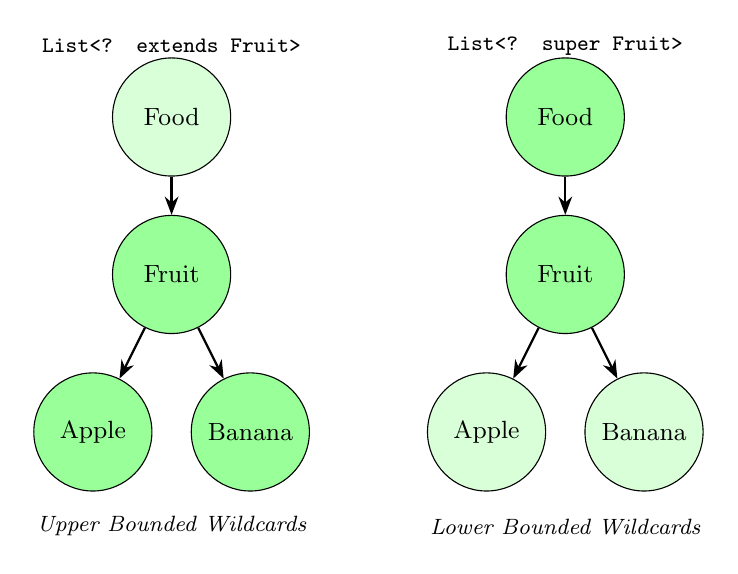
\begin{tikzpicture}[
    node/.style={draw, circle, minimum size=1.5cm, align=center,
                 fill=green!15, font=\small},
    selected/.style={draw, circle, minimum size=1.5cm, align=center,
                     fill=green!40, font=\small},
    arr/.style={-{Stealth}, thick},
  ]
  % Upper bounded --- left side
  \node[node]    (food1)  at (0,0)   {Food};
  \node[selected](fruit1) at (0,-2)  {Fruit};
  \node[selected](apple1) at (-1,-4) {Apple};
  \node[selected](ban1)   at (1,-4)  {Banana};
  \draw[arr] (food1)  -- (fruit1);
  \draw[arr] (fruit1) -- (apple1);
  \draw[arr] (fruit1) -- (ban1);
  \node[font=\footnotesize] at (0, 0.9)
    {\texttt{List<? extends Fruit>}};
  \node[font=\footnotesize\itshape] at (0,-5.2)
    {Upper Bounded Wildcards};

  % Lower bounded --- right side
  \node[selected](food2)  at (5,0)   {Food};
  \node[selected](fruit2) at (5,-2)  {Fruit};
  \node[node]    (apple2) at (4,-4)  {Apple};
  \node[node]    (ban2)   at (6,-4)  {Banana};
  \draw[arr] (food2)  -- (fruit2);
  \draw[arr] (fruit2) -- (apple2);
  \draw[arr] (fruit2) -- (ban2);
  \node[font=\footnotesize] at (5, 0.9)
    {\texttt{List<? super Fruit>}};
  \node[font=\footnotesize\itshape] at (5,-5.2)
    {Lower Bounded Wildcards};
\end{tikzpicture}%
}
\caption{Java generic wildcards.  Shaded nodes indicate which types are accepted by each
         wildcard form.}
\label{fig:ch10-wildcards}
\end{figure}

\subsection{Type Parameter Naming Conventions}
\label{subsec:ch10-naming}

The Java standard follows single-letter, upper-case type parameter names:
\texttt{E}~(Element), \texttt{K}~(Key), \texttt{V}~(Value), \texttt{N}~(Number),
\texttt{T}~(Type), and \texttt{S}, \texttt{U}, \texttt{V} for additional parameters.

\begin{keyresult}[title={Key Result: Benefits of Generics}]
Generics provide (1)~\textbf{compile-time type safety} — wrong types are caught before
runtime; (2)~\textbf{no explicit casting} on retrieval; (3)~\textbf{reusable code} —
one generic class serves many types.
\end{keyresult}

% ─────────────────────────────────────────────────────────────────────────────
\section{Collections Enhancements (Java 5+)}
\label{sec:ch10-collections}

Java's Collections Framework provides a unified architecture for storing and manipulating
groups of objects.  The top-level hierarchy is:

% [Figure, Slide 16: Full Java Collections Framework hierarchy. Iterable <- Collection
%  <- {List, Queue, Set}; Map is a separate branch. Concrete classes include ArrayList,
%  LinkedList, Vector/Stack under List; PriorityQueue, Deque/ArrayDeque under Queue;
%  HashSet, LinkedHashSet, SortedSet/TreeSet under Set; HashMap, LinkedHashMap, Hashtable,
%  SortedMap/TreeMap under Map.]
The root interface \texttt{Iterable<E>} enables the enhanced \texttt{for} loop.
\texttt{Collection<E>} extends it and is the parent of the three main sub-interfaces:
\textbf{List} (ordered, duplicates allowed — \texttt{ArrayList}, \texttt{LinkedList},
\texttt{Vector}/\texttt{Stack}), \textbf{Queue} (FIFO ordering —
\texttt{PriorityQueue}, \texttt{Deque}/\texttt{ArrayDeque}), and \textbf{Set} (no
duplicates — \texttt{HashSet}, \texttt{LinkedHashSet}, \texttt{SortedSet}/\texttt{TreeSet}).
The \textbf{Map} interface (\texttt{HashMap}, \texttt{LinkedHashMap}, \texttt{Hashtable},
\texttt{TreeMap}) is separate from \texttt{Collection} but still part of the framework.

With Generics, all collection types became parameterised in Java~5, replacing
\texttt{add(Object)} with \texttt{add(E)} and \texttt{get(int):Object} with
\texttt{get(int):E}.  This eliminated unsafe casts throughout collection usage.

% ─────────────────────────────────────────────────────────────────────────────
\section{Enhanced For Loop (Java 5)}
\label{sec:ch10-enhanced-for}

Java~5 introduced four main ways to traverse a collection, each suited to different needs.

\subsection{Basic For Loop (Index-Based)}
\label{subsec:ch10-basic-for}
\begin{lstlisting}[language=Java]
List<String> list = Arrays.asList("Apple", "Banana", "Cherry");
for (int i = 0; i < list.size(); i++) {
    System.out.println(list.get(i));
}
\end{lstlisting}
Best for index-based access (e.g.\ when the position of the element matters).

\subsection{Enhanced For-Each Loop}
\label{subsec:ch10-foreach}

Syntax: \texttt{for (Type variable : collection) \{ \ldots \}}

\begin{lstlisting}[language=Java]
List<String> list = Arrays.asList("Apple", "Banana", "Cherry");
for (String fruit : list) {
    System.out.println(fruit);
}
\end{lstlisting}

The loop variable (\texttt{fruit}) holds the current element; \texttt{Type} is its
declared type; \texttt{collection} is any array or \texttt{Iterable}.  Modifications
to the collection are not permitted during this loop.

\subsection{Iterator (Safe Element Removal)}
\label{subsec:ch10-iterator}
\begin{lstlisting}[language=Java]
Iterator<String> iterator = list.iterator();
while (iterator.hasNext()) {
    String fruit = iterator.next();
    System.out.println(fruit);
    if (fruit.equals("Banana")) {
        iterator.remove(); // safe removal during iteration
    }
}
\end{lstlisting}

\begin{warning}[title={Warning: \texttt{ConcurrentModificationException}}]
Never call \texttt{list.remove()} inside an enhanced \texttt{for} loop or while
iterating with an \texttt{Iterator}.  Always use \texttt{iterator.remove()} to
delete elements during iteration.
\end{warning}

\subsection{Stream API \texttt{forEach} (Functional, Java 8)}
\label{subsec:ch10-stream-foreach}
\begin{lstlisting}[language=Java]
list.stream().forEach(item -> System.out.println("Element: " + item));
\end{lstlisting}
\texttt{.stream()} creates a stream; \texttt{.forEach()} consumes each element via
a lambda.  Covered in detail in Section~\ref{sec:ch10-streams}.

% ─────────────────────────────────────────────────────────────────────────────
\section{Lambda Expressions (Java 8)}
\label{sec:ch10-lambdas}

\subsection{Motivation}
\label{subsec:ch10-lambda-motivation}

Before Java~8, passing behaviour required creating a full class or an anonymous inner
class.  Lambda expressions reduce this to a concise one-liner.

\begin{example}[Three equivalent approaches]
Traditional named class:
\begin{lstlisting}[language=Java]
public class HelloWorld {
    public void sayHello() { System.out.println("Hello, World!"); }
}
\end{lstlisting}
Anonymous inner class:
\begin{lstlisting}[language=Java]
Greeting greeting = new Greeting() {
    public void sayHello() { System.out.println("Hello, World!"); }
};
greeting.sayHello();
\end{lstlisting}
Lambda expression:
\begin{lstlisting}[language=Java]
Greeting greeting = () -> System.out.println("Hello, World!");
greeting.sayHello();
\end{lstlisting}
\end{example}

\subsection{Syntax}
\label{subsec:ch10-lambda-syntax}

\begin{definition}[Lambda Expression]
\label{def:ch10-lambda}
A lambda expression has the form:
\[
  \texttt{(arguments)} \;\texttt{->}\; \texttt{\{\ body\ \}}
\]
consisting of an \emph{argument list}, the \textbf{arrow token} \texttt{->}, and a
\emph{body}.
\end{definition}

Common forms:

\begin{lstlisting}[language=Java]
// No arguments
() -> System.out.println("Hello")

// One argument (parentheses optional)
s -> System.out.println(s)

// Two arguments
(x, y) -> x + y

// Explicit argument types
(Integer x, Integer y) -> x + y

// Multiple statements -- braces and return required
(x, y) -> {
    System.out.println(x);
    System.out.println(y);
    return x + y;
}
\end{lstlisting}

\subsection{Functional Interfaces}
\label{subsec:ch10-functional-interfaces}

A lambda can only be assigned to a \emph{functional interface} — an interface with exactly
one abstract method (annotated \texttt{@FunctionalInterface}).  Examples from
\texttt{java.util.function}: \texttt{Runnable} (\texttt{run()}), \texttt{Consumer<T>}
(\texttt{accept(T)}), \texttt{BiConsumer<T,U>} (\texttt{accept(T,U)}),
\texttt{Function<T,R>} (\texttt{apply(T)}), \texttt{BiFunction<T,U,R>}.

\begin{example}[\texttt{BiConsumer} with a lambda]
\leavevmode
\begin{lstlisting}[language=Java]
import java.util.function.BiConsumer;

BiConsumer<Integer, String> myLambda =
    (arg1, arg2) -> System.out.println(
        "Two arguments: " + arg1 + " and " + arg2);

myLambda.accept(5, "Hello");
// Output: Two arguments: 5 and Hello
\end{lstlisting}
\end{example}

\subsection{Method References}
\label{subsec:ch10-method-references}

When a lambda simply delegates to an existing method, a \emph{method reference}
(using \texttt{::}) is more concise.  There are five kinds:

\begin{center}
\begin{tabularx}{\linewidth}{llX}
\toprule
\textbf{Type} & \textbf{Example} & \textbf{Lambda equivalent} \\
\midrule
Static              & \texttt{Integer::parseInt}      & \texttt{str -> Integer.parseInt(str)} \\
Bound instance      & \texttt{Instant.now()::isAfter} & \texttt{t -> Instant.now().isAfter(t)} \\
Unbound instance    & \texttt{String::toLowerCase}    & \texttt{str -> str.toLowerCase()} \\
Class constructor   & \texttt{TreeMap<K,V>::new}      & \texttt{() -> new TreeMap<K,V>()} \\
Array constructor   & \texttt{int[]::new}             & \texttt{len -> new int[len]} \\
\bottomrule
\end{tabularx}
\end{center}

\begin{examtip}[title={Exam Tip: Lambda Best Practices}]
Keep lambdas short and focused on a single action.  Use method references wherever
possible (\texttt{System.out::println} instead of \texttt{x -> System.out.println(x)}).
Avoid placing complex logic inside a lambda body --- extract it into a named method.
\end{examtip}

% ─────────────────────────────────────────────────────────────────────────────
\section{Streams API (Java 8)}
\label{sec:ch10-streams}

\subsection{What is a Stream?}
\label{subsec:ch10-stream-what}

\begin{definition}[Java Stream]
\label{def:ch10-stream}
A \textbf{stream} is a sequence of elements from a source (array, collection, I/O
channel) that supports aggregate, functional-style operations via a
\emph{stream pipeline}: source $\rightarrow$ intermediate operations $\rightarrow$
terminal operation.
\end{definition}

% [Figure, Slide 37: Stream pipeline diagram. A data source (cylinder labelled "Array,
%  Collection, I/O channel") feeds into a "Create Stream Instance" box, then into a
%  dashed rectangle labelled "Stream Pipeline" containing N intermediate operation gears
%  (filter, map, sort, ...) chained together, leading to a "Terminal Operation" box, then
%  to an "Operation Result" document icon (count, sum, collected collection).]
The pipeline model is: a \emph{source} generates a stream instance; zero or more
\emph{intermediate operations} (lazy, return a new stream) transform the data;
a single \emph{terminal operation} (eager, triggers execution) produces a result.

Key properties of streams are shown in Table~\ref{tab:ch10-stream-features}.

\begin{table}[h]
\centering
\begin{tabularx}{\linewidth}{lX}
\toprule
\textbf{Feature} & \textbf{Description} \\
\midrule
No stored data       & Process data from existing sources; never store it. \\
Immutable processing & Original data is not modified; a new result is produced. \\
Lazy evaluation      & Intermediate operations execute only when a terminal operation is invoked. \\
Method chaining      & Operations return streams, enabling concise pipeline syntax. \\
Intermediate ops     & \texttt{filter()}, \texttt{map()}, \texttt{sorted()}, \texttt{distinct()} --- return a stream. \\
Terminal ops         & \texttt{collect()}, \texttt{forEach()}, \texttt{reduce()}, \texttt{count()} --- produce a result. \\
Parallel processing  & \texttt{.parallelStream()} splits work across threads automatically. \\
\bottomrule
\end{tabularx}
\caption{Key features of Java Streams.}
\label{tab:ch10-stream-features}
\end{table}

\subsection{Stream Operations}
\label{subsec:ch10-stream-ops}

\begin{example}[\texttt{filter} --- keep elements matching a predicate]
\leavevmode
\begin{lstlisting}[language=Java]
List<String> names = Arrays.asList("Alice", "Bob", "Charlie");
List<String> filtered = names.stream()
    .filter(name -> name.startsWith("A"))
    .collect(Collectors.toList()); // [Alice]
\end{lstlisting}
\end{example}

\begin{example}[\texttt{map} --- transform each element]
\leavevmode
\begin{lstlisting}[language=Java]
List<Integer> numbers = Arrays.asList(1, 2, 3, 4);
List<Integer> squared = numbers.stream()
    .map(n -> n * n)
    .collect(Collectors.toList()); // [1, 4, 9, 16]
\end{lstlisting}
\end{example}

\begin{example}[\texttt{sorted} --- sort in natural order]
\leavevmode
\begin{lstlisting}[language=Java]
List<String> sortedNames = names.stream()
    .sorted()
    .collect(Collectors.toList());
\end{lstlisting}
\end{example}

\begin{example}[\texttt{forEach} --- terminal operation, consumes each element]
\leavevmode
\begin{lstlisting}[language=Java]
names.stream().forEach(System.out::println);
\end{lstlisting}
\end{example}

\begin{example}[\texttt{collect} --- aggregate into a collection]
\leavevmode
\begin{lstlisting}[language=Java]
List<String> result = names.stream()
    .filter(name -> name.length() > 3)
    .collect(Collectors.toList());
\end{lstlisting}
\end{example}

\begin{example}[Parallel stream]
\leavevmode
\begin{lstlisting}[language=Java]
List<Integer> parallelResult = numbers.parallelStream()
    .map(n -> n * n)
    .collect(Collectors.toList());
\end{lstlisting}
\end{example}

\begin{example}[Chained pipeline --- filter, map, sort, distinct]
\leavevmode
\begin{lstlisting}[language=Java]
List<String> names = Arrays.asList("Alice", "Bob", "Charlie", "David");
List<String> finalResult = names.stream()
    .filter(n -> n.startsWith("A"))
    .map(String::toUpperCase)   // method reference
    .sorted()
    .distinct()
    .collect(Collectors.toList()); // [ALICE]
\end{lstlisting}
\end{example}

\begin{keyresult}[title={Key Result: Streams vs.\ Loops}]
Streams do not replace loops entirely, but excel at data transformation pipelines
where multiple filter/map/sort operations are chained.  Lazy evaluation means unused
intermediate results are never computed.  Use \texttt{parallelStream()} for large
datasets, but be aware of thread-safety constraints on shared state.
\end{keyresult}

% ─────────────────────────────────────────────────────────────────────────────
\section{Default Methods in Interfaces (Java 8)}
\label{sec:ch10-default-methods}

\subsection{What is a Default Method?}
\label{subsec:ch10-default-what}

\begin{definition}[Default Method]
\label{def:ch10-default}
A \textbf{default method} is a method declared inside an interface with the
\texttt{default} keyword and a concrete body.  Implementing classes inherit the
default implementation and may override it.
\end{definition}

\begin{example}[\texttt{Vehicle} interface with a default method]
\leavevmode
\begin{lstlisting}[language=Java]
interface Vehicle {
    void start(); // abstract -- must be implemented

    default void stop() {
        System.out.println("Vehicle is stopping.");
    }
}
\end{lstlisting}
\end{example}

\subsection{Why Are Default Methods Needed?}
\label{subsec:ch10-default-why}

Before Java~8, adding a new method to a published interface broke all existing
implementations --- they would no longer compile.  Default methods allow interfaces
to evolve (e.g.\ the \texttt{forEach} and \texttt{stream} methods added to
\texttt{Collection} in Java~8) without breaking code that already implements them.

\begin{example}[Extending \texttt{Printer} without breaking implementations]
\leavevmode
\begin{lstlisting}[language=Java]
interface Printer {
    void print();

    // New in v2 -- existing implementors are unaffected:
    default void scan() {
        System.out.println("Scanning document...");
    }
}
\end{lstlisting}
\end{example}

\subsection{Resolving Default Method Conflicts (Multiple Inheritance)}
\label{subsec:ch10-default-conflict}

A class may implement two interfaces that both declare a default method with the same
signature.  The class \emph{must} override that method to resolve the ambiguity, and
may call either interface's version via \texttt{InterfaceName.super.method()}:

\begin{example}[Resolving a default method conflict]
\leavevmode
\begin{lstlisting}[language=Java]
interface A {
    default void show() { System.out.println("A"); }
}
interface B {
    default void show() { System.out.println("B"); }
}
class C implements A, B {
    @Override
    public void show() {
        System.out.println("Resolving conflict");
        A.super.show(); // explicitly delegates to A
    }
}
\end{lstlisting}
\end{example}

\subsection{Static Methods in Interfaces}
\label{subsec:ch10-static-interface}

Java~8 also allows \texttt{static} methods in interfaces.  They are not inherited by
implementing classes and must be called via the interface name:

\begin{lstlisting}[language=Java]
interface Utility {
    static void displayMessage() {
        System.out.println("Static interface method.");
    }
}
// Call: Utility.displayMessage();
\end{lstlisting}

\begin{keyresult}[title={Key Result: Interface Method Types (Java 8+)}]
\begin{center}
\begin{tabularx}{\linewidth}{lXl}
\toprule
\textbf{Feature}  & \textbf{Purpose} & \textbf{Overridable?} \\
\midrule
Abstract method   & Must be implemented by the class             & Yes \\
Default method    & Adds new methods without breaking existing code & Yes \\
Static method     & Utility/helper function on the interface     & No  \\
\bottomrule
\end{tabularx}
\end{center}
\end{keyresult}

% ─────────────────────────────────────────────────────────────────────────────
\section{Enhanced Switch (Java 12+)}
\label{sec:ch10-switch}

\subsection{Limitations of the Traditional Switch}
\label{subsec:ch10-switch-traditional}

The traditional \texttt{switch} statement has two well-known pitfalls:
\emph{fall-through} (execution continues past a matched case unless \texttt{break} is
written) and verbosity (a separate \texttt{break} and assignment are required for each
case).

\begin{lstlisting}[language=Java]
int num;
switch (day) {
    case MONDAY: num = 1; break;
    case TUESDAY: num = 2; break;
    default: num = 0;
}
\end{lstlisting}

\subsection{Enhanced Switch Expression}
\label{subsec:ch10-switch-enhanced}

Java~12 introduced \emph{switch expressions} with \textbf{arrow labels} (\texttt{->}),
which eliminate fall-through and can be used directly as expressions:

\begin{lstlisting}[language=Java]
int num = switch (day) {
    case MONDAY  -> 1;
    case TUESDAY -> 2;
    default      -> 0;
};
\end{lstlisting}

Multiple labels can be combined in one case:

\begin{lstlisting}[language=Java]
int result = switch (grade) {
    case 'A', 'B' -> 100;
    case 'C'      -> 75;
    default       -> 50;
};
\end{lstlisting}

\subsection{The \texttt{yield} Statement}
\label{subsec:ch10-yield}

When a case branch requires multiple statements, use a block with \texttt{yield} to
return a value:

\begin{lstlisting}[language=Java]
int finalScore = switch (grade) {
    case 'A' -> {
        System.out.println("Excellent");
        yield 100; // returns value from block
    }
    case 'B' -> 85;
    default  -> 50;
};
\end{lstlisting}

\subsection{Using Enhanced Switch with Enums}
\label{subsec:ch10-switch-enum}

The enhanced switch pairs naturally with enums, as all cases are known at compile time:

\begin{lstlisting}[language=Java]
enum Day { MONDAY, TUESDAY, WEDNESDAY,
           THURSDAY, FRIDAY, SATURDAY, SUNDAY }

String activity = switch (day) {
    case SATURDAY, SUNDAY -> "Relax";
    default               -> "Work";
};
\end{lstlisting}

\begin{keyresult}[title={Key Result: Enhanced Switch Benefits}]
\begin{itemize}[nosep]
  \item \textbf{No fall-through} --- each arrow case is independent.
  \item \textbf{Expression support} --- the result can be assigned directly to a
        variable.
  \item \textbf{Concise syntax} --- fewer lines, no repeated \texttt{break}.
  \item \textbf{Exhaustiveness} (with enums/sealed types) --- the compiler warns if
        cases are missing.
\end{itemize}
\end{keyresult}

% ─────────────────────────────────────────────────────────────────────────────
\section{Summary}
\label{sec:ch10-summary}

\begin{center}
\begin{tabularx}{\linewidth}{llX}
\toprule
\textbf{Java version} & \textbf{Feature} & \textbf{Main benefit} \\
\midrule
Java 5  & Generics              & Compile-time type safety; no explicit casts \\
Java 5  & Collections enhancements & Parameterised collections (\texttt{List<E>}, etc.) \\
Java 5  & Enhanced \texttt{for} & Cleaner iteration over arrays and collections \\
Java 7  & Diamond operator      & Type inference on the right-hand side \\
Java 8  & Lambda expressions    & Concise inline behaviour; functional interfaces \\
Java 8  & Streams API           & Declarative data pipelines with lazy evaluation \\
Java 8  & Default methods       & Interface evolution without breaking existing code \\
Java 12+ & Enhanced \texttt{switch} & Expression-style switch; no fall-through \\
\bottomrule
\end{tabularx}
\end{center}

\end{document}
